%% LyX 2.0.5 created this file.  For more info, see http://www.lyx.org/.
%% Do not edit unless you really know what you are doing.
\documentclass[12pt,oneside,A4paper]{book}
\usepackage[T1]{fontenc}
\usepackage{geometry}
\geometry{verbose,tmargin=3cm,bmargin=3cm,lmargin=4cm,rmargin=2.5cm}
\setcounter{secnumdepth}{3}
\setcounter{tocdepth}{3}
\usepackage{prettyref}
\usepackage{refstyle}
\usepackage{float}
\usepackage{enumitem}
\usepackage{amsthm}
\usepackage{amsmath}
\usepackage{amssymb}
\usepackage{graphicx}
\usepackage{setspace}
\usepackage{esint}
\onehalfspacing
\usepackage[unicode=true,pdfusetitle,
 bookmarks=true,bookmarksnumbered=true,bookmarksopen=false,
 breaklinks=false,pdfborder={0 0 1},backref=false,colorlinks=false]
 {hyperref}

\makeatletter

%%%%%%%%%%%%%%%%%%%%%%%%%%%%%% LyX specific LaTeX commands.

\AtBeginDocument{\providecommand\eqref[1]{\ref{eq:#1}}}
\AtBeginDocument{\providecommand\secref[1]{\ref{sec:#1}}}
%% Because html converters don't know tabularnewline
\providecommand{\tabularnewline}{\\}
%% A simple dot to overcome graphicx limitations
\newcommand{\lyxdot}{.}

\floatstyle{ruled}
\newfloat{algorithm}{tbp}{loa}[chapter]
\providecommand{\algorithmname}{Algorithm}
\floatname{algorithm}{\protect\algorithmname}
\RS@ifundefined{subref}
  {\def\RSsubtxt{section~}\newref{sub}{name = \RSsubtxt}}
  {}
\RS@ifundefined{thmref}
  {\def\RSthmtxt{theorem~}\newref{thm}{name = \RSthmtxt}}
  {}
\RS@ifundefined{lemref}
  {\def\RSlemtxt{lemma~}\newref{lem}{name = \RSlemtxt}}
  {}


%%%%%%%%%%%%%%%%%%%%%%%%%%%%%% Textclass specific LaTeX commands.
\numberwithin{equation}{section}
\numberwithin{figure}{section}
\numberwithin{table}{section}
  \theoremstyle{definition}
  \newtheorem{defn}{\protect\definitionname}[section]
  \theoremstyle{plain}
  \newtheorem{thm}{\protect\theoremname}[section]
  \theoremstyle{plain}
  \newtheorem{lem}{\protect\lemmaname}[section]
 \newlist{casenv}{enumerate}{4}
 \setlist[casenv]{leftmargin=*,align=left,widest={iiii}}
 \setlist[casenv,1]{label={{\itshape\ \casename} \arabic*.},ref=\arabic*}
 \setlist[casenv,2]{label={{\itshape\ \casename} \roman*.},ref=\roman*}
 \setlist[casenv,3]{label={{\itshape\ \casename\ \alph*.}},ref=\alph*}
 \setlist[casenv,4]{label={{\itshape\ \casename} \arabic*.},ref=\arabic*}
  \theoremstyle{plain}
  \newtheorem{cor}{\protect\corollaryname}[section]

\@ifundefined{showcaptionsetup}{}{%
 \PassOptionsToPackage{caption=false}{subfig}}
\usepackage{subfig}
\makeatother

  \providecommand{\definitionname}{Definition}
  \providecommand{\lemmaname}{Lemma}
 \providecommand{\casename}{Case}
\providecommand{\corollaryname}{Corollary}
\providecommand{\theoremname}{Theorem}

\begin{document}

\title{\thispagestyle{empty}%\pagestyle{empty} %multiple pagesOptimized
Distributed Average Consensus Algorithm and its Applications }

\maketitle

\chapter*{ }

\newenvironment{acknowledgements} {\pagestyle{empty}   \begin{center} 
%\vspace*{1.5cm} 
{\Large \bfseries Acknowledgements} \end{center} 
%\vspace{0.5cm} 
\begin{quote}} {\end{quote} }

\begin{acknowledgements} 



\begin{doublespace}
 







I would like to express my gratitude to my thesis advisor Prof. Xinheng
Wang for his careful guidance and his valuable comments; his patience
and the constructive criticism helped me to organize many concepts
in a frame. His encouragement has been invaluable. thank you so much
Henry!

I would also like to thank Prof. Choi for his insightful comments
their suggestions contributed to board my view of the distributed
information system and the distributed consensus problem. Thank you
for your help and encouragement.

 

Thanks to my colleagues Frank Liu, Tommy To, Laurie Hughes, John Li.

 

At last, I would like to sincerely thank my parents, for their encouragement
and support during all phases of this work.
\end{doublespace}

\end{acknowledgements}



\chapter*{}

\newenvironment{abstract} {  \pagestyle{empty}   \begin{center}   
%\vspace*{1.5cm}   
{\Large \bfseries  Abstract}   \end{center}  
%\vspace{0.5cm}   
\begin{quote}} {\end{quote} }

\begin{abstract} 

\thispagestyle{empty}Distributed information processing has attract
more interest recently because its advantages in distributed network
than centralized method. One of the tools of distributed signal processing
is the distributed consensus algorithm. If the consensus algorithm
is to find the average value over the network, the algorithm is called
the distributed average consensus (DAC), which is an matrix iterative
algorithm to find the dominant eigenvector of the matrix. Generally,
the algorithm is required to return the result more quickly so that
the distributed system can have a higher data processing performance.
Therefore, many efforts have been devoted into the optimization of
the distributed average algorithm. However, most of the optimization
are centralized method so the system can not be optimized in a distributed
network. In addition, the existing distributed optimization algorithm
converges very slowly. 

Consequently, we proposed a distributed real-time optimization for
the DAC algorithms. The optimization has advantages in low computation
time and can work simultaneously with the consensus algorithm. Later,
an application of cloud detection is given where optimized DAC algorithms
are applied to perform the hypothesis testing. Simulation result shows
that the DAC algorithm using centralized optimization and proposed
optimization have similar performances in convergence rate, when floating
point number with double format is used and the network size is less
than 32. In addition, the performances of the detection system with
different number of sensors are plotted using relative operating characteristic
curves. It is shown that the detection system with more sensors can
have better performance. 



\end{abstract}


\pagenumbering{roman}

\tableofcontents{}

\listoffigures


\addcontentsline{toc}{chapter}{List of Figures}

\listoftables


\addcontentsline{toc}{chapter}{List of Tables}


\chapter*{Abbreviations}

%\chapter*{Abbreviations} %[List of Abbreviations]
\addcontentsline{toc}{chapter}{List of Abbreviations}
% \begin{thenomenclature} 
% \begin{abbreviations}{WidestAbbreviation} 
% \begin{itemize} 
\begin{tabular}{p{4.0cm} p{11cm}}2D &  Two Dimensional \\
3D &  Three Dimensional\\
WSNs &  Wireless Sensor Netoworks\\
DAC Algorithm &  Distributed Average Consensus Algorithm\\
FIR filter &  Finite Impulse Response Filter\\
FO-DAC Algorithm &  First-order Distributed Average Consensus Algorithm\\
HO-DAC Algorithm &  Higher-order Distributed Average Consensus Algorithm\\
CFO-DAC Algorithm &  Constant First Order Distributed Average Consensus
Algorithm\\
FT-DAC Algorithm &  Finite Time Distributed Average Consensus Algorithm\\
LLR  &  Log Likelihood ratio\\


\end{tabular}


\chapter*{Notations}

%\chapter*{Notations} %[List of Notations]
\addcontentsline{toc}{chapter}{List of Notations}
%\begin{listofsymbols} 
\begin{tabular}{p{2.5cm} p{11cm}} %\begin{abmbreviations}{WidestAbbreviation}
% \nomgroup{A}





${\cal G}$  &  Graph associated to the network \\


$\mathcal{V}$  &  Set of nodes $\mathcal{V}=\left\{ v_{1},v_{2},...,v_{n}\right\} $
in the graph ${\cal G}$\\


$\mathcal{E}$  &  Set of edges $\mathcal{E}\subseteq\mathcal{V}\times\mathcal{V}$
in the graph ${\cal G}$\\


${\cal A}$  &  Weighted adjacency associated with graph ${\cal G}$\\


$W$  &  Weight matrix of first-order DAC algorithm \\


$w_{ij}$  &  Entry of weight matrix $W$\\


$\mathbf{H}$  &  weight matrix of higher-order DAC algorithm \\


$\lambda_{i}\left(W\right)$ &  The $i^{th}$ Eigenvalue of weight
matrix $W$\\


$S\left(W\right)$  &  Spectrum of of the matrix $W$\\


\textit{$Q$ } &  Incidence matrix associated with graph ${\cal G}$\\


$L$  &  Laplacian matrix induced by ${\cal G}$\\


$l_{ij}$  &  Entry of Laplacian matrix $L$\\


$\lambda_{i}\left(L\right)$ &  The $i^{th}$ Eigenvalue of Laplacian
matrix $L=L\left({\cal G}\right)$\\


$S\left(L\right)$  &  Spectrum of the Laplacian matrix\\


$\mathbf{x}\left(k\right)$  &  Local value vector at time index
$k$\\


$x_{i}\left(k\right)$  &  Local value of node $i$ at time index
$k$\\


$\epsilon$ &  Step length of DAC algorithms\\


$\gamma$ &  Forgetting factor of DAC algorithms\\


$\epsilon_{opt,FO}$ &  Optimal step length of first-order DAC algorithms\\


$\epsilon_{opt,SO}$ &  Optimal step length of second-order DAC algorithms\\


$\gamma_{opt,SO}$ &  Optimal forgetting factor of second-order DAC
algorithms\\


$p(\lambda)$  &  The minimal polynomial of $W$ \\


$T_{i}\left(k,D_{i}\right)$  &  Toeplitz matrix in $\mathbb{R}^{D_{i}\times D_{i}}$
at $v_{i}$ with $x_{i}\left(k\right)$ as diagonal entries.\\


$\mathbf{y}_{i}\left(k,D_{i}\right)$  &  The local value history
vector at $v_{i}$ constructed by $\left[x_{i}\left(k+1\right),x_{i}\left(k+2\right),\ldots,x_{i}\left(k+D_{i}\right)\right]^{T}$
\\


$\mathbf{h}$  &  An FIR filter that can estimate the consensus value
\\


\end{tabular} 
%\end{listofsymbols}


\pagenumbering{arabic}
%\pagestyle{fancy} 
\setcounter{page}{1}


\chapter{Introduction }



































Due to the development of wireless sensor networks and the decreasing
cost of sensor nodes,  processing information that originally  acquired
by the nodes is often necessary. As any node only has a piece of local
information,  all information need to be gathered and processed at
a special node called  fusion center. This method is intuitive  and
is called centralized signal processing. 

However, fusion center is usually the most important and expense node
in the network. Once it is destroyed or failed, the whole network
breaks down. In addition, as data gathering is an energy consuming
process, centralized signal processing is limited due to energy constrain
of mobile nodes. Moreover, there is unbalance energy consumption between
nodes with different communication loads \cite{Cristescu2004}\cite{Yuen2008}. 

Distributed signal processing has become more attractive, as it can
be robust against  nodes failure or topology changes \cite{Chair1986}
. However, not all the signal processing can be distributed many processing
algorithm are still implemented by centralized method.

Distributed average consensus (DAC) algorithm is a tool for distributed
information processing. It has received significant attention recently
because of its robustness and simplicity. It is widely used in many
applications such as time synchronization \cite{Schenato2011}, rendezvous
\cite{Ren2008}, cooperative control of vehicles \cite{Yang2010},
formation control/flocking \cite{Olfati-Saber2012} and WSNs \cite{Hlinka2012}.
In these applications, it is often necessary that a group of nodes
can agree on certain quantities. 



In different applications, DAC algorithms may also need a little modification.
For example, in distributed tracking of a moving target by wireless
sensor networks. Suppose each sensor is observing the target coordinates
but the output is corrupted by independent and identically distributed
zero-mean Gaussian noise, to minimize the interference from the noise,
the sensors need to take the average of all initial values. In distributed
hypothesis testing, the goal is to find the production of the global
likelihood ratio which is the product of the local likelihood ratio.
Therefore, each sensor first calculate the log of the local likelihood
ratio and substitute it into the DAC algorithm. The average obtained
by DAC algorithm multiplied with the number of nodes in the network
is log of global likelihood ratio.

In practice, DAC algorithms also face the challenges of link failure,
time delay, dynamic network, asynchronous communication and other
practical aspects. Therefore, a simple but reliable solution sometimes
performs better. First-order DAC algorithms have been proved to be
robust against  topology changes and they play important roles in
practice \cite{Ren2007}. Its optimization in a dynamic network still
attract lots of interest \cite{Jakovetic2010}\cite{Nedic2010}. 


\section{Motivation of Research }

The research is motivated by the distributed detection of cloud detection
using WSN. One of the properties of mobile sensor nodes is the limited
energy capacity. Therefore, to minimize the power consumption of the
sensor nodes, DAC algorithm to perform the distributed signal processing
need to be optimized. In addition, the model of cloud requires a modification
because the sensor is using laser sensing technology. It emit a laser
to illuminate the cloud and collect the backscatters to sense the
cloud concentration.


\subsection{To Find a Faster DAC Algorithm. }

  

In the distributed tracking of a moving target, when the moving target
is highly dynamic or the sensors need to sample at a very high frequency,
it requires that the DAC algorithm returns the result in a short time.
Thus, many efforts have been devoted to optimize the algorithm. 

DAC algorithms can be divided into asymptotic and non-asymptotic algorithms.
For asymptotic algorithms, the optimization is to minimize the sub-dominate
eigenvalue of a weight matrix \cite{Asensio-Marco2012}\cite{Xiao2004}\cite{Xiong2010}.
 However, these optimization of DAC algorithms are centralized methods
. 

For non-asymptotic DAC algorithms, such as finite-time \cite{Sundaram2007}
and adaptive filter DAC algorithm \cite{Cavalcante2010}, the optimization
is to minimize the number of necessary iteration before a FIR filter
is estimated. Sumdaram and Hadjicostis \cite{Sundaram2007} verify
that there exists a FIR filter that can estimate the consensus value.
Cavalcante and Mulgrew \cite{Cavalcante2010} follow Sundaram and
Hadjicostis's work to propose an adaptive algorithm to find the filter.
However, they are not robust against topology changes.   Local values
over time obtained by the first-order DAC are taken as inputs of the
filter estimation algorithm for both of them. As a result, if the
network topology changes, these algorithms have to be reinitialized,
as outdated information during the filter estimation will lead to
a wrong answer.

To enable the whole system work distributively, the DAC algorithms
should be robust against topology changes and the optimization should
be distributed. 

A distributed method inspired by the gossip algorithm \cite{Boyd2006}
can be used to optimize the first order DAC but it converges very
slowly. The method involves triple nested distributed matrix iterations.
The inner iteration has to converge to a certain range so that the
iteration outside can return the right result. Thus, It is not surprising
that it could not finish in a reasonable time when the network size
is large. 

Therefore, a distributed optimization method with less computation
time is required. In addition, it is better that no additional communication
cost is required. Moreover, if the optimization algorithm and the
DAC algorithm can be executed simultaneously, then consensus process
will not be interrupted and the optimization can be running in background
to keep the optimal parameters updated in a dynamic network. 


\subsection{To Detect The Cloud Plume by Laser Sensor}

The cloud here is a group of harmful gas or particles floating in
the air. To detect the cloud, it is illuminated by a laser beam emitted
by a sensor and the backscatters (light reflected by particles) are
collected to generate signals. 

Because the laser beam penetrate the cloud, the intensity of backscatters
is the integration along the laser beam in that range. Consequently,
a new cloud plume model need to be obtained by take integration of
original Gaussian plume model along the direction of laser beam. 

Specifically, in the cloud detection application, the DAC algorithm
performs the task of distributed hypothesis testing may also have
a little modification. To find the production of the global likelihood
ratio, each sensor first calculate the log of the local likelihood
ratio and substitute it into the DAC algorithm as the initial local
value. DAC algorithm will then find the average. The average multiplied
by the number of nodes in the network is log of global likelihood
ratio.


\section{Contributions}

The main contribution of this thesis is that it proposed a distributed
real-time optimization method, which will not interrupt the constant
first-order DAC algorithm. Thus, the consensus algorithm and the optimization
method can be executed simultaneously. As a result, communication
cost and optimization initialization time can be dramatically reduced
compare to conventional distributed optimization. In addition, a least
mean square solution is obtained to mitigate the numerical error of
the optimal solution calculated by the proposed method. When using
floating point number in double format and the network size is smaller
than 32, the numerical error after mitigation does not dramatically
decline the algorithm performance. 

In addition, the proposed distributed eigenvalue estimation algorithm
could be an alternative to the estimation of algebra connectivity,
such as \cite{Yang2010}. The proposed method could obtain the result
with sufficient numerical accuracy. Matrix iterations only need to
be executed for times in order of $n$. 

Moreover, we propose a generalized finite-time DAC algorithm, which
does not require knowledge of network topology but will estimate the
necessary parameters during the iteration. Compared to the distributed
algorithm introduced in \cite{Sundaram2007}, it doesn't require the
re-initialization of the constant first-order DAC algorithm for several
times. Therefore, total data transmission in all iterations can be
reduced. However, re-initialization can be introduced if the consensus
value requires to have high accuracy 

Finally, a modified Gaussian plume models is presented, which is the
integration of the original Gaussian plume model along the laser beam
to simulate the laser penetration. This Gaussian plume model can only
describe the mean of the cloud concentration. However, a real cloud
cloud concentration is actually a random process. To reveal  the dynamics
and turbulence properties of the cloud plume, a 3D cloud animation
is implemented with the computer graphic technology \cite{He2011}. A
bunch of the simulated cloud plumes is generated for algorithm testing
and detection.




\section{Outline}

This thesis is structured as follows: Chapter  \ref{sec:Consensus-problem-on}
is the review of some asymptotic and non-asymptotic DAC algorithms,
as well as some distributed signal processing methods based on DAC
algorithm. In chapter  \ref{sub:Finite-time-Consensus-on}, a generalized
finite-time DAC algorithm will be presented. Compared to the previous
version of finite-time DAC, the number of iteration can be reduced.
In chapter \ref{sec:Online-Optimization-of}, a distributed real-time
optimization method to increase the convergence rate of asymptotic
DAC algorithms. Finally, a distributed detection of cloud plume using
wireless sensor networks and the DAC algorithm will be introduced
in chapter \ref{sec:DAC-Implementation:-Distributed}. Chapter \ref{sec:Conclusion-and-Future}
concludes this thesis and gives out the direction of further work.



\section{\label{sec:Consensus-problem-on}Consensus problem on Graphs (todo)}

Consider a network (connected graph) $\mathcal{G}=\left(\mathcal{V},\mathcal{E},{\cal A}\right)$
be a weighted digraph (or undirected graph) consisted by a set of
nodes $\mathcal{V}=\left\{ 1,2,...,n\right\} $, a set of edges $\mathcal{E}\subseteq\mathcal{V}\times\mathcal{V}$
and a weighted adjacency matrix ${\cal A}=\left[a_{ij}\right]$. The
edge $\left(i,j\right)\in\mathfrak{\mathcal{E}}$ is an unordered
pair of distinct nodes, associated with an element in the adjacency
matrix ${\cal A}$, i.e. $\left(i,j\right)\in\mathfrak{\mathcal{E}}\Leftrightarrow a_{ij}$.
we assume $a_{ij}=0$, if $j\notin{\cal N}_{i}$ (note that $a_{ii}=0$,
as $i\notin{\cal N}_{i}$) for all $i\in\mathcal{V}$.. Moreover,
the set of neighbors of node $i$ is denoted by $\mathcal{N}_{i}=\text{ }\left\{ j\in{\cal V}|\left(i,j\right)\in\mathcal{E}\right\} $,
an node $i$ can only transmit information to other nodes that belong
to the neighbors set. (OK1)

Suppose each node holds an initial scalar value $x_{i}\left(0\right)\in R$,
which can be a value that locally acquired by node representing physical
quantities including temperature, humidity, illumination, attitude,
and so on. We define the local value vector $\mathbf{x}\left(0\right)=\left[x_{1}\left(0\right),...,x_{n}\left(0\right)\right]^{T}\in R^{n}$
to represent all the initial values on the network. The network is
said to be reached a consensus if and only if $x_{i}=x_{j}$, for
all nodes $i,j\in{\cal V},i\neq j$. In the other words, all the nodes
of the network are in an agreement, the common value of all nodes
is called the consensus value. (OK1)

To describe the behavior of each node or agent, suppose each node
has the following dynamics 

\begin{equation}
\dot{x}_{i}=f\left(x_{i},u_{i}\right),i\in{\cal V}
\end{equation}
and the graph (or network) is a system has the dynamics

\begin{equation}
\mathbf{\dot{x}}=F\left(\mathbf{x},\mathbf{u}\right)\label{eq:system dynamic}
\end{equation}
where $F\left(\mathbf{x},\mathbf{u}\right)$ is the columnwise concatenation
of individual dynamics $f\left(x_{i},u_{i}\right)$, for all node
$i=1,\ldots,n$. In an ad-hoc network with the mobile nodes, the topology
$G$\textbf{ }is switching and the system will updating its $F\left(\mathbf{x},\mathbf{u}\right)$
from time to time. 

The input or feedback $u_{i}$ in the node's dynamic is a function
of the historical states of node $i$ and its neighbors
\begin{equation}
u_{i}=g\left(x_{j_{1}},x_{j_{2}},\ldots,x_{j_{m_{i}}}\right)\label{eq:consensus protocol}
\end{equation}
where $j_{1},\ldots,j_{m_{i}}$ are the node indexes that belong to
the set $\left\{ i\right\} \cup{\cal N}_{i}$. \prettyref{eq:consensus protocol}
is called a consensus protocol under topology $G$. If the network
graph is not fully connected, it is said to be a distributive consensus
protocol. 
\begin{defn}
Let ${\cal X}:R^{n}\to R$ be a function of $n$ variables of $x_{1},x_{2},\ldots,x_{n}$
and let $\mathbf{x}\left(0\right)$ denotes the initial condition
of the network. The ${\cal X}$-consensus problem is a distributive
method to calculate the consensus value ${\cal X}\left(\mathbf{x}\left(0\right)\right)$
in a graph $G$. 
\end{defn}
Actually, there are different consensus problems too. For instance,
the average consensus ${\cal X}\left(\mathbf{x}\right)=\frac{1}{n}\sum_{i=1}^{n}x_{i}\left(0\right)$,
maximum consensus ${\cal X}\left(\mathbf{x}\right)=\max\left(\mathbf{x}\right)$,
minimum consensus ${\cal X}\left(\mathbf{x}\right)=\min\left(\mathbf{x}\right)$
and variance consensus ${\cal X}\left(\mathbf{x}\right)=\mbox{var}\left(\mathbf{x}\right)$
are given by their expressions respectively. The average consensus
is a special case of consensus problem, which computing the average
of all initial values $\overline{x}=\mbox{mean}\left(\mathbf{x}\right)=\frac{1}{n}\sum_{i=1}^{n}x_{i}\left(0\right)$
using a distributive system dynamics $\mathbf{\dot{x}}=F\left(\mathbf{x},\mathbf{u}\right)$
in a network $G$.(OK1)

We are interested in the distributive solutions of the consensus problem
as the network only allows an node to communicate with its neighbors.
We say the protocol \prettyref{eq:consensus protocol} solves the
consensus problem asymptotically if and only if there exists an asymptotically
stable state $x^{*}={\cal X}\left(\mathbf{x}\right)$ of system dynamics
\prettyref{eq:system dynamic}, which satisfying for all $\delta>0$,
there exists a time index $t^{*}>0$, such that $\left|x_{i}(t)-x^{*}\right|<\delta$
for all $t>t^{*}$ and $\forall i\in{\cal V}$.

The average consensus problem is much challenge than the maximum consensus
(or minimum consensus), since it relates a linear combination of all
the initial states of network nodes and the condition $x_{i}^{*}={\cal X}\left(\mathbf{x}\right)$
for all nodes $i$ has to be satisfied. Furthermore, the variance
consensus problem can be solved by two instances of average consensus,
because we have the relation $\mbox{var}\left(\mathbf{x}\right)=\mbox{mean}\left(\mathbf{x}\cdot\mathbf{x}\right)-\left[\mbox{mean}\left(\mathbf{x}\right)\right]^{2}$.
Thus, in the following of this thesis we focus on the average consensus
problem and the distributed average consensus (DAC) algorithms. (OK1)


\subsection{Continuous-time vs. Discrete-time Consensus}

In this section, we illustrate consensus protocol 
\begin{equation}
u_{i}\left(t\right)=\sum_{j\in{\cal N}_{i}}a_{ij}\left(x_{j}-x_{i}\right)\label{eq:1st Order Protocol}
\end{equation}
that solves the average consensus problem ${\cal X}\left(\mathbf{x}\right)=\mbox{mean}\left(\mathbf{x}\right)$
and show the difference and similarity of continuous-time with the
dynamics 

\begin{equation}
\dot{x}_{i}\left(t\right)=u_{i}\left(t\right)\label{eq:continuous-time consensus}
\end{equation}
and discrete-time consensus with the dynamics 
\begin{equation}
x_{i}\left(k+1\right)=x_{i}\left(k\right)+u_{i}\left(k\right)\label{eq:discre-time consensus}
\end{equation}


The continuous-time consensus requires the nodes in a network have
dynamics in a form of differential equations while nodes in the discrete-time
consensus has dynamics in difference equation. Continuous-time consensus
involves analog signals that are easily interfered by channel noise.
Consequently, the finally consensus value will be a random variable
with mean equals to the consensus value without noise and variance
proportional to the signal noise ratio. It is shown in \cite{Kar2009},
the variance is also proportional to time $t$ hence it is increasing
as the algorithm executing. 

(todo give a simulation with channel noise)

Without the channel noise, the system dynamics with the feedback in
\ref{eq:1st Order Protocol} can evolve into a linear system with
differential equation given by 
\begin{equation}
\mathbf{\dot{x}}\left(t\right)=-{\cal L}\mathbf{x}\left(t\right)\label{eq:system differential dynamics}
\end{equation}
Solving the differential equation \ref{eq:system differential dynamics}
will yield a continuous-time solution in an exponential matrices form
\begin{equation}
\mathbf{x}\left(t\right)=\exp\left(-{\cal L}t\right)\mathbf{x}\left(0\right)\label{eq:x(t) of CT-1st-DAC}
\end{equation}
where ${\cal L}$ is called the weighted graph Laplacian associated
with network graph ${\cal G}$, which is defined by

\begin{equation}
l_{ij}=\begin{cases}
\sum_{k=1,k\neq i}^{n}a_{ik} & j=i\\
-a_{ij} & j\neq i
\end{cases}\label{eq:Graph Laplacian def.}
\end{equation}
For a graph with 0-1 adjacency, the graph Laplacian can be denoted
in another form, which is unweighted Laplacian matrix denoted by $\mathbf{L}$

\begin{equation}
l_{ij}=\begin{cases}
\left|{\cal N}_{i}\right| & j=i\\
-1 & j\in{\cal N}_{i}\\
0 & \mbox{otherwise}
\end{cases}\label{eq:Laplacian def.}
\end{equation}
In some literature for example \cite{Xiong2009a}, they use the second
definition (\prettyref{eq:Laplacian def.}) of the Laplacian matrix
to analyze the convergence rate of DAC algorithm. It is a special
case when weights $a_{ij}$ for all edges in ${\cal E}$ equal to
one. Therefore, to distinguish them, we denote the weighted graph
Laplacian matrix and the unweighted Laplacian matrix by ${\cal L}$
and $\mathbf{L}$ respectively. 

On the other hand, discrete-time consensus only involves the quantization
error during the algorithm execution as long as the data packages
are correctly received. Nowadays, sensor nodes with digital processing
unit becomes more cheaper, we can get more benefits from the advantages
of discrete-time consensus algorithms. Consequently, discrete-time
consensus algorithms are mainly discussed in the following of this
thesis. 

For network agents have discrete-time consensus protocol, their system
dynamics can be given in a matrix form
\begin{equation}
\mathbf{x}(k+1)=\mathbf{W}\mathbf{x}(k)
\end{equation}
where $\mathbf{W}=\left[w_{ij}\right]=I-{\cal L}$. We say the iteration
is convergent if there exists a vector denoted by $\mathbf{x}^{*}$,
which satisfies.

\begin{equation}
\mathbf{x}^{*}=\mathbf{W}\mathbf{x}^{*}\label{eq:stable state iteration}
\end{equation}
Moreover, 

\begin{equation}
\mathbf{x}(k+1)-\mathbf{x}^{*}=\mathbf{W}\left[\mathbf{x}(k)-\mathbf{x}^{*}\right]\label{eq:error vector iter. 1st}
\end{equation}
\prettyref{eq:stable state iteration} states that $\mathbf{x}^{*}$
is a right eigenvector of matrix $\mathbf{W}$ associated to a simple
eigenvalue 1. For more details about the discrete-time first-order
DAC algorithm, see \prettyref{sub:DT-First-Order-DAC}. 



\section{Asymptotic Distributed Consensus Algorithm}

The averaging consensus problem can be solved not only by DAC algorithms,
but also in many other ways, such as flooding, gossip and so on. In
the flooding algorithm, each sensor maintains a table of all sensors
values which initialize by its local value. At each iteration of the
flooding algorithm, every node exchanges the table with their neighbors.
After enough steps, which is larger than the diameter of the network.
Every node will get all the initial value of all nodes. Gossip algorithms
are asynchronous. Only one random node wakes up and randomly chooses
another node. The two nodes exchange their estimates and update to
the average of the two. 

Due to the simplicity and robustness of asymptotic distributed consensus
algorithm, it plays an important role in the practical problems. They
are already applied to network with a large number of nodes and proofed
to be robust against the topology variation. Once the network graph
is strong connected, the convergence to global consensus value is
guaranteed \cite{Ren2007}. In this section, we start from the first-order
DAC algorithm and then expand the algorithm to higher-order in order
to yields a higher the convergence rate.


\subsection{\label{sub:DT-First-Order-DAC}Discrete First Order Distributed Consensus
Algorithm}

First Order Distributed Consensus Algorithm (FO-DCA) update the local
value of node $i$ iteratively at each time-step $k$ by a weighted
sum of node\textquoteright{}s local values one time step before, given
by 

\begin{eqnarray}
x_{i}(k+1) & = & x_{i}(k)+\sum_{j\in\mathcal{N}_{i}}w_{ij}\left[x_{j}(k)-x_{i}(k)\right]\label{eq:1st iter. ni}\\
 & = & w_{ii}x_{i}(k)+\sum_{j\in\mathcal{N}_{i}}w_{ij}x_{j}(k)
\end{eqnarray}
where $k=0,1,2,...$ is the time index, $w_{ij}$ is the weight to
$x_{j}$ at node $i$, $w_{ij}=0$ if $(i,j)\notin\mathcal{E}$. Note
that we define a weight to node $i$ itself $w_{ii}=1-\sum_{j\in\mathcal{N}_{i}}w_{ij}$,
so that the sum of all weights equals to one, $\sum_{j=1}^{n}w_{ij}=1$. 

The iteration \prettyref{eq:1st iter. ni} can be written in a vector
form 

\begin{equation}
\mathbf{x}(k+1)=W\mathbf{x}(k)\label{eq:first order matrix}
\end{equation}
where $W$ is a weight matrix which refer to as the Perron matrix
induced by ${\cal G}$ \cite{Olfati-Saber2004}. This linear iteration
implies that $\mathbf{x}(k)=W^{k}\mathbf{x}(0)$ for $k=1,2,\cdots$. 

Since the initial value vector is randomly chosen, the matrix $W$
must satisfy some convergence conditions to make sure the iteration
convergent, and the convergence rate depends on the spectral radius
of matrix $W$.


\subsubsection{Convergence Conditions}

For the matrix iteration defined in \prettyref{eq:first order matrix},
the average consensus problem is to choose the weight matrix $W$,
so that for any initial value $\mathbf{x}(0)\in R^{n}$, $\mathbf{x}(k)$
converges to the vector 

\begin{equation}
\mathbf{\bar{x}}=\left(\mathbf{1}^{\mathrm{T}}\mathbf{x}(0)/n\right)\mathbf{1}=\dfrac{\mathbf{11}^{\mathrm{T}}}{n}\mathbf{x}(0)
\end{equation}

\begin{thm}
\cite{Xiao2004}\textup{\label{thm:convergence condition}$\lim_{k\rightarrow\infty}\mathbf{x}(k)=\mathbf{\bar{x}}$}
if and only if the matrix $W$ satisfie\textup{s
\begin{equation}
\lim_{k\rightarrow\infty}W^{k}=\dfrac{\mathbf{11}^{\mathrm{T}}}{n}.\label{eq:convege condition W}
\end{equation}
}Eq.\prettyref{eq:convege condition W} holds if and only if
\begin{eqnarray}
\mathbf{1}^{\mathrm{T}}W & = & \mathbf{1}^{\mathrm{T}}\label{eq: Converge condition W_Left}\\
W\mathbf{1} & = & \mathbf{1}\label{eq: Converge condition W_right}\\
\rho\left(W-\mathbf{11}^{\mathrm{T}}/n\right) & < & 1\label{eq:Converge cond. rhu<1}
\end{eqnarray}
where vector $\mathbf{1}=[1,1,\cdots1,]^{\mathrm{T}}\in R^{n}$, $\rho\left(\cdot\right)$
denotes the spectral radius of the matrix .
\end{thm}
Eq.\prettyref{eq: Converge condition W_Left} means that has a left
eigenvector $\mathbf{1}$ associated with the eigenvalue 1. This implies
that the sum of local value vector is not changed in the iteration
$\sum_{i\in\mathcal{V}}x_{i}\left(k+1\right)=\sum_{i\in\mathcal{V}}x_{i}\left(k\right)$
and the sum of each column of matrix $W$ is equal to one. Eq.\prettyref{eq: Converge condition W_right}
shows that $W$ is a row stochastic matrix and has an eigenvalue 1
with associated eigenvector $\mathbf{1}$. Both \prettyref{eq: Converge condition W_Left}
and \prettyref{eq: Converge condition W_right} together with the
convergence condition \prettyref{eq:Converge cond. rhu<1} means that
$W$ have a simple eigenvalue equals to one, and modular of all other
eigenvalues are less than one.
\begin{lem}
\textup{\label{thm:Share the eigenvalues}If $\lim_{k\rightarrow\infty}W^{k}=\dfrac{\mathbf{11}^{\mathrm{T}}}{n}$,
the matrix $W-\mathbf{11}^{\mathrm{T}}/n$ share the same eigenvalues
as matrix $W$ except the simple eigenvalue one is replaced by zero.}\end{lem}
\begin{proof}
Eq.\prettyref{eq: Converge condition W_Left} implies that the matrix $W$
has a left eigenvector $\mathbf{1}$ associated with eigenvalue one.
And Eq.\prettyref{eq: Converge condition W_right} implies that $\mathbf{1}$
is a right eigenvector of $W$ associated with eigenvalue one. The
fact that $\lim_{k\rightarrow\infty}W^{k}=\dfrac{\mathbf{11}^{\mathrm{T}}}{n}$
exists if and only if there exists a  matrix $U$ and $W$ can be
Jordan decomposition as 
\begin{equation}
W=U\left[\begin{array}{cccc}
J_{1}\\
 & J_{2}\\
 &  & \ddots\\
 &  &  & J_{m}
\end{array}\right]U^{-1}
\end{equation}
where $m$ is the number of distinct Jordan block. $J_{i}$ is the
$r_{i}$ dimensional Jordan block corresponding to eigenvalue $\lambda_{i}$,
$J_{1}=I_{r_{1}}$ is the $r_{i}$ dimensional identity matrix $\left(0\leq r_{i}\leq n\right)$
and all other Jordan block are convergent, i.e. $\rho\left(J_{i}\right)<1,2\leq i\leq m$.

Let $u_{1},u_{2},\ldots,u_{n}$ be the column of $U$ and $v_{1}^{T},v_{2}^{T},\ldots,v_{n}^{T}$
be row of $U^{-1}$. Then we have 
\begin{eqnarray}
\lim_{k\to\infty}W^{k} & = & U\left[\begin{array}{cc}
I_{r_{1}} & 0\\
0 & 0
\end{array}\right]U^{-1}\label{eq: W^k to infinity has Rank one}\\
 & = & \sum_{i=1}^{r_{1}}u_{i}v_{i}^{T}=\dfrac{\mathbf{11}^{\mathrm{T}}}{n}\label{eq:u*v=00003D11}
\end{eqnarray}
As the property of unitary matrix $U$, both $u_{i}$ and $v_{i}$
are set of orthogonal normal vectors, each $u_{i}v_{i}^{T}$ is a
matrix with rank one and matrix $\sum_{i=1}^{n}u_{i}v_{i}^{T}$ has
rank $n$. The sum $\sum_{i=1}^{r_{1}}u_{i}v_{i}^{T}$ must have rank
$r_{1}.$ Eq.\prettyref{eq:u*v=00003D11} shows that $r_{1}$ must equal
to one and $u_{i}v_{i}^{T}=\dfrac{\mathbf{11}^{\mathrm{T}}}{n}$,
both $u_{i}$ and $v_{i}$ are vectors with the same constant on all
components. Therefore, $W-\dfrac{\mathbf{11}^{\mathrm{T}}}{n}$ have
the same Jordan decomposition as $W$ except the Jordan block $J_{1}$
is replaced by zero, and all other Jordan block remain the same. This
completes the proof. 
\end{proof}
The convergence rate of the FO-DCA is related to the spectral radius
of matrix $W-\dfrac{\mathbf{11}^{\mathrm{T}}}{n}$. To get the maximum
convergence rate, an optimization problem to minimize the spectral
radius of the matrix could be solved \cite{Xiao2004}. 

\begin{equation}
\begin{array}{ccc}
\mbox{\mbox{Minimize }} & \rho\left(W-\frac{\mathbf{1}\mathbf{1}^{T}}{n}\right)\\
\mbox{Subject to } & \mathbf{1}^{\mathrm{T}}W=\mathbf{1}^{\mathrm{T}},\; W\mathbf{1}=\mathbf{1} & ,
\end{array}\label{eq: Opt. FO-DAC Problem}
\end{equation}
But it requires knowledge of network topology to solve the problem.
However, some non-optimal convergent weight matrices that satisfy
the condition in Eq.\prettyref{eq:convege condition W} are given
below. 


\subsubsection{First-order DAC Based On a Constant}

The simplest way to choose a weight matrix set all edges symmetric
and their weights equal to the constant $\epsilon$. A special weight
to a node itself is chosen to be $1-\epsilon\left|\mathcal{N}_{i}\right|$,
so that the sum of weights at a node is one. Therefore, the weight
matrix can be defined by the Laplacian matrix 
\begin{equation}
W=I_{n}-\epsilon L\label{eq:def. const FO-DAC}
\end{equation}
where the constant $\epsilon$ is the \textit{step length}. This kind
of DAC algorithm is called the \textit{constant FO-DAC}.

Let $\mathbf{e}_{1},\mathbf{e}_{2},\ldots,\mathbf{e}_{n}$ be the
eigenvectors of $W$ and $\lambda_{1}\left(W\right),\lambda_{2}\left(W\right),\ldots,\lambda_{n}\left(W\right)$
be the associated eigenvalues and they are ordered so that $1=\left|\lambda_{1}\left(W\right)\right|\geq\left|\lambda_{2}\left(W\right)\right|\geq\ldots\geq\left|\lambda_{n}\left(W\right)\right|$.
The largest eigenvalue $\lambda_{1}\left(W\right)$ is called the
\textit{dominant eigenvalue} and associated eigenvector $\mathbf{e}_{1}$
is called the \textit{dominant eigenvector}. 

From Eq.\prettyref{eq:def. const FO-DAC}, the eigenvalues of these
two matrix $W$ and $L$ have relationship given by $\lambda_{i}\left(W\right)=1-\epsilon\lambda_{i}\left(L\right)$.
Thus, we can determine the convergence range of $\epsilon$ in terms
of $\lambda\left(L\right)$.


\paragraph*{Choosing the step length}

For the constant FO-DAC algorithm, it is convergent, if and only if
the step length $\epsilon$ is in the range $\left(0,2/\lambda_{n}\left(L\right)\right)$.
And the optimal step length which maximize the convergence rate is
$\epsilon{}_{opt,FO}=\frac{2}{\lambda_{2}\left(L\right)+\lambda_{n}\left(L\right)}$
\cite{Xiao2004}. The boundary of the dominant eigenvalue $\lambda_{n}\left(L\right)$
can be found in \cite{Russell1994}, given by $d_{max}+1\leq\lambda_{n}\left(L\right)\leq\max\left\{ d_{u}+d_{v}\right\} $,
where $\left(u,v\right)\in{\cal E}$ , $d_{u}$ is the degree of node
$v_{u}$ and $d_{max}=\max_{v_{i}\in{\cal V}}\left|{\cal N}_{i}\right|$
is the maximum degree of nodes in the network. By Gerschgorin's theorem,
we have another upper boundary of $\lambda_{n}\left(L\right)\leq2d_{max}$,
then convergence is guaranteed if $\epsilon\in\left(0,1/d_{max}\right]$. 


\subsubsection{First Order DAC based on local degree}

Another option is Metropolis weight matrix (or local degree weight
matrix), where each weight is determined by degree of the two nodes
on the edge,

\begin{equation}
w_{ij}=\begin{cases}
\frac{1}{1+\max\left\{ d(i),d(j)\right\} }, & \mbox{if }(i,j)\in\mathit{\mathcal{E}}\\
1-\sum_{(i,k)\in\mathit{\mathcal{E}}}w_{ik}, & i=j\\
0, & \mbox{otherwise}
\end{cases}
\end{equation}
where $d(i)$ and $d(j)$ are the degrees of nodes $i$ and $j$. 

As shown above, the conventional DAC algorithm is depends on eigenvalues
of graph Laplacian matrix $\lambda_{i}\left(L\right)$ or degree of
nodes. However, in the section \ref{sub:Finite-time-Consensus-on},
we will show that the finite-time DAC algorithm in an invariant network
doesn't require these prior knowledge, if $\mathbf{x}\left(k\right)$
can be represented by a linear combination of a new normal basis defined
by eigenvectors of $W$. Thus, the weight matrix doesn't have too
much requirements and can be more easily chosen. This would be very
applicable because nodes in a distributed network usually doesn't
have any knowledge of network topology. 


\subsection{\label{sub:Discrete-High-Order}Discrete High Order Distributed Consensus
Algorithm }

Higher order Distributed Consensus Algorithm (HO-DCA) can have faster
convergence rate and potentially faster than FO-DCA. It can be easily
implemented by storing and using past data, and doesn't require additional
communication and network configuration. Moreover, HO-DAC can be regard
as a generalized form of distributed consensus algorithm \cite{Xiong2010}.
In \cite{Xiong2010}, the author assume all node can store and using
past data and define a topology-dependent matrix to update the initial
data. It involves more parameters than FO-DAC so that the optimization
problem has more degrees of freedom. When some parameters are set
to zero, the HO-DCA algorithm can reduce to the best constant FO-DAC
algorithm.

Since the convergence rate of the initial values is related to eigenvalues
of Laplacian matrix. In the optimization problem of HO-DCA, eigenvalues
of the associated graph Laplacian matrix or weight matrix must known. 

In a time-invariant, connected network, the $M-th$ high-order DAC
algorithm has the form:
\begin{eqnarray}
x_{i}(k) & = & x_{i}(k-1)-\epsilon\sum_{m=1}^{M}c_{m}(-\gamma)^{m-1}\Delta x_{i}(k,m),\label{eq:Iteration Second order x_i(k)}\\
\Delta x_{i}(k,m) & = & \sum_{j\in\mathcal{N}_{i}}\left(x_{i}\left(k-m\right)-x_{j}\left(k-m\right)\right),
\end{eqnarray}
Where $x_{i}(k)$ is the local value at node $i$ during iteration
$k$; $\mathcal{N}_{i}$ is the neighboring nodes set in which the
nodes can communicate reliably with node $i$; $\epsilon$ is a constant
step size; $M$ is the highest order number; $c_{m}$ are predefined
constants, where $c_{1}=1$ and $c_{m}\neq0\:(m>1)$; $\gamma$ is
a forgetting factor, such that $\left|\gamma\right|<1$. 

Define

\begin{equation}
\mathbf{x}(k)=\left[x_{1}(k),x_{1}(k),\ldots,x_{n}(k)\right]^{T}
\end{equation}
The Eq.\prettyref{eq:Iteration Second order x_i(k)} can be written in matrix
form

\begin{equation}
\mathbf{x}(k)=(I_{n}-\epsilon L)\mathbf{x}(k-1)-\epsilon\sum_{m=2}^{M}c_{m}(-\gamma)^{m-1}L\mathbf{x}(k-m)\label{eq:High Order Iter.Vec}
\end{equation}
where $L$ is the Laplacian matrix associated with the network graph.
assume $\forall k<0,\;\mathbf{x}(k)=\mathbf{x}(0)$, $\mathbf{x}(0)$
is the initial local state information for node $i$. The matrix form
states that when the forgetting factor $\gamma$ is set to zero, the
HO-DAC is reduced into the best constant FO-DAC algorithm given in 

Simulation result shows that, a higher order will have better convergence
rate, but should be trade off with the algorithm complexity and computational
cost. Also only a few improvement could be achieved if we introduce
larger than fourth order. 


\subsubsection{Convergence Rate Maximization Problem For HO-DAC}

Based on the iteration equation \ref{eq:High Order Iter.Vec}, the
$M-th$ high-order DAC algorithm in a time-invariant, connected and
undirected network, with initial local value vectors $\mathbf{x}(-M+1)=,\ldots,=\mathbf{x}(-1)=\mathbf{x}(0)$,
can be further defined by an $Mn\times Mn$ matrices
\begin{equation}
\mathbf{H}=\left[\begin{array}{cccc}
I_{n}-\epsilon L & c_{2}\gamma\epsilon L & \cdots & -c_{M}(-\gamma)^{M-1}\epsilon L\\
I_{n} & \mathbf{0}_{n\times n} & \cdots & \mathbf{0}_{n\times n}\\
\vdots & \ddots &  & \vdots\\
\mathbf{0}_{n\times n} & \cdots & I_{n} & \mathbf{0}_{n\times n}
\end{array}\right]
\end{equation}
\begin{equation}
\mathbf{J}=\left[\begin{array}{cccc}
\mathbf{K} & \mathbf{0}_{n\times n} & \cdots & \mathbf{0}_{n\times n}\\
\mathbf{K} & \mathbf{0}_{n\times n} & \cdots & \mathbf{0}_{n\times n}\\
\vdots & \vdots & \ddots & \vdots\\
\mathbf{K} & \mathbf{0}_{n\times n} & \cdots & \mathbf{0}_{n\times n}
\end{array}\right]
\end{equation}
 where $\mathbf{K}=\left(\frac{1}{n}\right)\mathbf{1}\mathbf{1}^{T}$,
and $\mathbf{0}_{n\times n}$ denotes the $n\times n$ all-zero matrix. 

The high-order DAC algorithm with initial condition $\mathbf{x}(-M+1)=,\ldots,=\mathbf{x}(-1)=\mathbf{x}(0)$
is convergent if and only if $\rho\left(\mathbf{H}-\mathbf{J}\right)<1$
\cite{Xiong2010}. Then a spectral radius minimization problem to
find the optimal $\epsilon$ and $\gamma$ for the high-order DAC
algorithm is formulated as

\begin{equation}
\begin{array}{cc}
\mbox{\mbox{Minimize }} & \rho\left(\mathbf{H}-\mathbf{J}\right)\\
\mbox{Subject to } & \epsilon,\gamma\in R
\end{array},\label{eq: High order spectral radius problem}
\end{equation}


As shown in Eq.\prettyref{eq: High order spectral radius problem},
the convergence rate maximization for high order DAC algorithm can
be cast into a spectral radius minimization problem. Finding the solution
is not easy due to we have to solve the high-order polynomial to calculate
eigenvalues. For example, the high-order polynomial of the eigenvalues
of $\mathbf{H-J}$ when $M=3$, $c_{1}=1$ and $c_{2}=1$ is 
\begin{equation}
f(\lambda)=\lambda^{3}-\left(1-\epsilon\lambda_{i}\left(L\right)\right)\lambda^{2}-\gamma\epsilon\lambda_{i}\left(L\right)\lambda+\gamma^{2}\epsilon\lambda_{i}\left(L\right)=0\label{eq: eigenvalue equation of H-J}
\end{equation}
where $\lambda_{i}(L)$ is the $i^{th}$ smallest eigenvalue of the
Laplacian Matrix \cite{Xiong2010}. 

Since each $\lambda_{i}(L),\; i=1,2,\cdots,n$ with generate one equation
which has $M$ roots, there are totally $M\times n$ eigenvalue for
$\mathbf{H-J}$. Then, problem Eq.\prettyref{eq: High order spectral radius problem}
can be written into minimize the maximum absolute value of all the
eigenvalues of $\mathbf{H-J}$. 
\begin{equation}
\begin{array}{cc}
\mbox{Minimize } & \mbox{max}\{\left|\lambda_{i}\left(\mathbf{H-J}\right)\right|\},\: i=1,2,\cdots,n\\
\mbox{Subject to } & \epsilon,\gamma\in R
\end{array},\label{eq:HO-DAC Opt. Problem}
\end{equation}



\subsubsection{Solve The Problem: Convergence rate maximization}

The convergence rate optimization problem \ref{eq:HO-DAC Opt. Problem}
of HO-DAC in undirected network can be graphically illustrated by
the \prettyref{fig:Find-minimum-rho(H)}, where the surface of $\mbox{max}\{\left|\lambda_{i}\left(\mathbf{H-J}\right)\right|\},\: i=1,2,\cdots,n$
is plotted and the optimal solution $\left(\epsilon{}_{opt},\gamma_{opt}\right)$
is marked with a star. We denote the optimized spectral radius by
$\rho_{opt}=\mbox{\mbox{min}}\rho\left\{ \left(\mathbf{H}-\mathbf{J}\right)\right\} $. 

Since the eigenvalues in the high-order polynomial \prettyref{eq: eigenvalue equation of H-J}
are network topology dependent, the solution of the problem \ref{eq:HO-DAC Opt. Problem}
may not have a unique analytical solution when the order is larger
than second. In this case, the problem will be solved numerically,
for example using steepest descent method. 

\begin{figure}
\hfill{}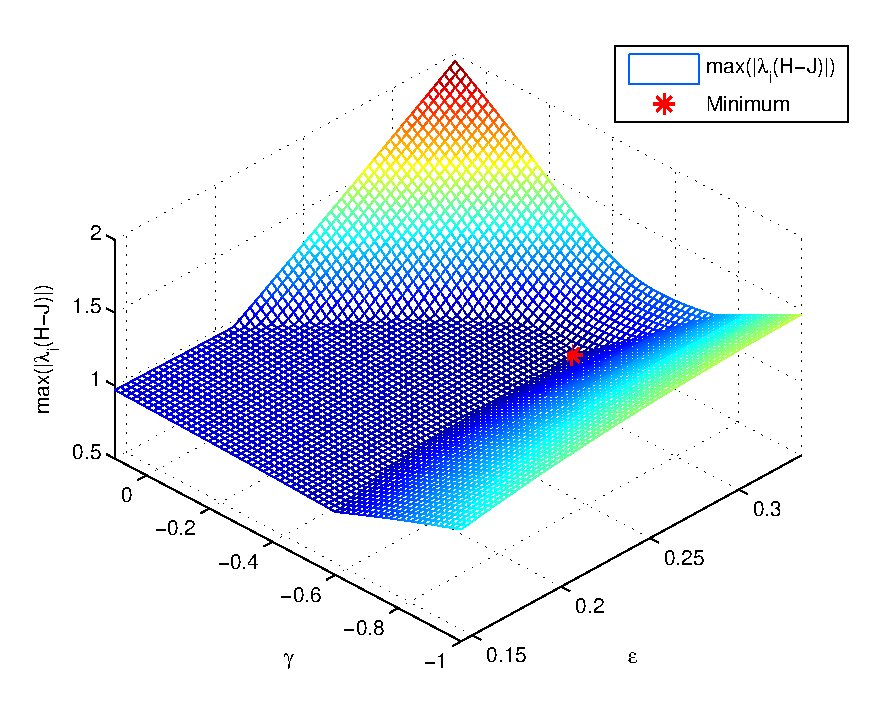
\includegraphics[height=9cm]{D:/Dropbox/PaperWork/FirstYearReport/Lyx_v/images/3order_max_lambda}\hfill{}\hfill{}\caption{\label{fig:Find-minimum-rho(H)} Illustration of Convergence rate
optimization, $\min\left\{ \mbox{max}\left[\lambda_{i}\left(\mathbf{H-J}\right)\right]\right\} ,\: i=1,2,\cdots,n$. }
\end{figure}


\begin{figure}
\hfill{}\includegraphics[height=9cm]{\string"Graph/Convergence region\string".pdf}\hfill{}\hfill{}\caption{\label{fig:Convergence-Region}Convergence Region for second order
DAC. }
\end{figure}


However, the second order DAC (SO-DAC), does exist an analytical solution.
As pointed out in \cite{Xiong2009a}, the convergence region for second
order DAC in undirected network which satisfy $\rho\left(\mathbf{H}-\mathbf{J}\right)<1$
is ${\cal R}={\cal R}_{1}\cup{\cal R}_{2}$, where 
\begin{eqnarray}
{\cal R}_{1} & = & \left\{ \frac{-1}{\epsilon\lambda_{n}\left(L\right)}<\gamma<1,0<\epsilon<\frac{1}{\lambda_{n}\left(L\right)}\right\} \\
{\cal R}_{2} & = & \left\{ \frac{-1}{\epsilon\lambda_{n}\left(L\right)}<\gamma<\frac{2}{\epsilon\lambda_{n}\left(L\right)}-1,\frac{1}{\lambda_{n}\left(L\right)}\leq\epsilon<\frac{3}{\lambda_{n}\left(L\right)}\right\} \label{eq:Def Convergence region R1 R2}
\end{eqnarray}
Fig.\ref{fig:Convergence-Region} graphically illustrate these region,
${\cal R}_{1}$ and ${\cal R}_{2}$ are defined in \prettyref{eq:Def Convergence region R1 R2}.
Note the dashed line separates the regions in which $\lambda_{n'}\left(\mathbf{H}\right),\lambda_{n"}\left(\mathbf{H}\right)$
are real and complex. In addition, optimal solution is always located
on this line. Moreover, the eigenvalues of $\mathbf{H}$ corresponding
to eigenvalue of $\lambda_{i}\left(L\right)$ is denoted by $\lambda_{i'}\left(\mathbf{H}\right)$
and $\lambda_{i"}\left(\mathbf{H}\right)$, which is 
\begin{eqnarray}
\lambda_{i'}\left(\mathbf{H}\right) & = & \frac{1}{2}\left[1-\epsilon\lambda_{i}\left(L\right)+\sqrt{\left(1-\epsilon\lambda_{i}\left(L\right)\right)^{2}+4\gamma\epsilon\lambda_{i}\left(L\right)}\right],\nonumber \\
\lambda_{i"}\left(\mathbf{H}\right) & = & \frac{1}{2}\left[1-\epsilon\lambda_{i}\left(L\right)-\sqrt{\left(1-\epsilon\lambda_{i}\left(L\right)\right)^{2}+4\gamma\epsilon\lambda_{i}\left(L\right)}\right].\label{eq:2nd-DAC lambda_H solution}
\end{eqnarray}
 

Since $\lambda_{2}\left(L\right)\leq\dots\leq\lambda_{n}\left(L\right)$,
in the convergence region of the second order DAC algorithm, the optimization
problem \prettyref{eq:HO-DAC Opt. Problem} can be equivalent to 
\[
\begin{array}{cc}
\mbox{Minimize } & \mbox{max}\{\left|\lambda_{2'}\left(\mathbf{H}\right)\right|,\left|\lambda_{2"}\left(\mathbf{H}\right)\right|,\left|\lambda_{n'}\left(\mathbf{H}\right)\right|,\left|\lambda_{n"}\left(\mathbf{H}\right)\right|\}\\
\mbox{Subject to } & \epsilon,\gamma\in R
\end{array},
\]


Finding the optimal solutions needs consideration of different combinations
of $\lambda_{2'}\left(\mathbf{H}\right),\lambda_{2"}\left(\mathbf{H}\right),\lambda_{n'}\left(\mathbf{H}\right),\lambda_{n"}\left(\mathbf{H}\right)$
when they are real value or complex value. However, for a connected
network, the $\lambda_{2'}\left(\mathbf{H}\right),\lambda_{2"}\left(\mathbf{H}\right)$
are real and $\lambda_{n'}\left(\mathbf{H}\right),\lambda_{n"}\left(\mathbf{H}\right)$
are complex values in the convergence region. When the minimum is
achieved, the following equation satisfied
\[
\left|\lambda_{2'}\left(\mathbf{H}\right)\right|=\left|\lambda_{n'}\left(\mathbf{H}\right)\right|=\left|\lambda_{n"}\left(\mathbf{H}\right)\right|
\]
Thus, by solving this equation, we have the optimal solution for second
order DAC algorithm.

\begin{eqnarray}
\epsilon{}_{opt,SO} & = & \frac{3\lambda_{n}(L)+\lambda_{2}(L)}{\lambda_{n}(L)\left[\lambda_{n}(L)+3\lambda_{2}(L)\right]}
\end{eqnarray}


\begin{equation}
\gamma_{opt,SO}=-\frac{\left[\lambda_{n}(L)-\lambda_{2}(L)\right]^{2}}{\left[\lambda_{n}(L)+3\lambda_{2}(L)\right]\left[3\lambda_{n}(L)+\lambda_{2}(L)\right]}
\end{equation}
These parameters could be floored to all sensors before the algorithm
start so that it converges faster.

Besides these results, we need to point out that the optimal solution
$\epsilon{}_{opt,SO}$ and $\gamma_{opt,SO}$ have the following relationship
\[
\gamma_{opt,SO}=\frac{\left[1-\epsilon{}_{opt,SO}\lambda_{n}\left(L\right)\right]^{2}}{-4\epsilon{}_{opt,SO}\lambda_{n}\left(L\right)}
\]
which implies the value under the square root in \prettyref{eq:2nd-DAC lambda_H solution}
is equal to zero, and $\lambda_{n'}\left(\mathbf{H}\right),\lambda_{n"}\left(\mathbf{H}\right)$
are all real values. Additionally, the optimal solution is located
just on the boundary of the regions where $\lambda_{n'}\left(\mathbf{H}\right),\lambda_{n"}\left(\mathbf{H}\right)$
is real and complex respectably, shown as dashed line in Fig. \ref{fig:Convergence-Region}. 


\subsection{Simulation and Algorithms Performance}

To test the performance of high-order DAC algorithm with different
orders, a simulation is carry out on 1000 random generated networks.
The methods and parameters of network generation are illustrated in
fig.\ref{fig:Net-N16-R0,3}. The algorithm's performance is evaluated
by the average spectral radius and average mean square error, shown
in \prettyref{fig:DAC-comparation}. 


\subsubsection{Random Network Generation}

The following is a simulation of network generation to show how the
wireless sensor networks is distributed. First, we randomly and uniformly
distribute a certain number of nodes in a unit square. Second, each
sensor randomly choose a local initial value has equally probability
density function. Finally, connect any two nodes if their satisfy
a certain communication constrains. 

\begin{figure}[h]
\hfill{}\subfloat[\label{fig:Net-N50-E200}]{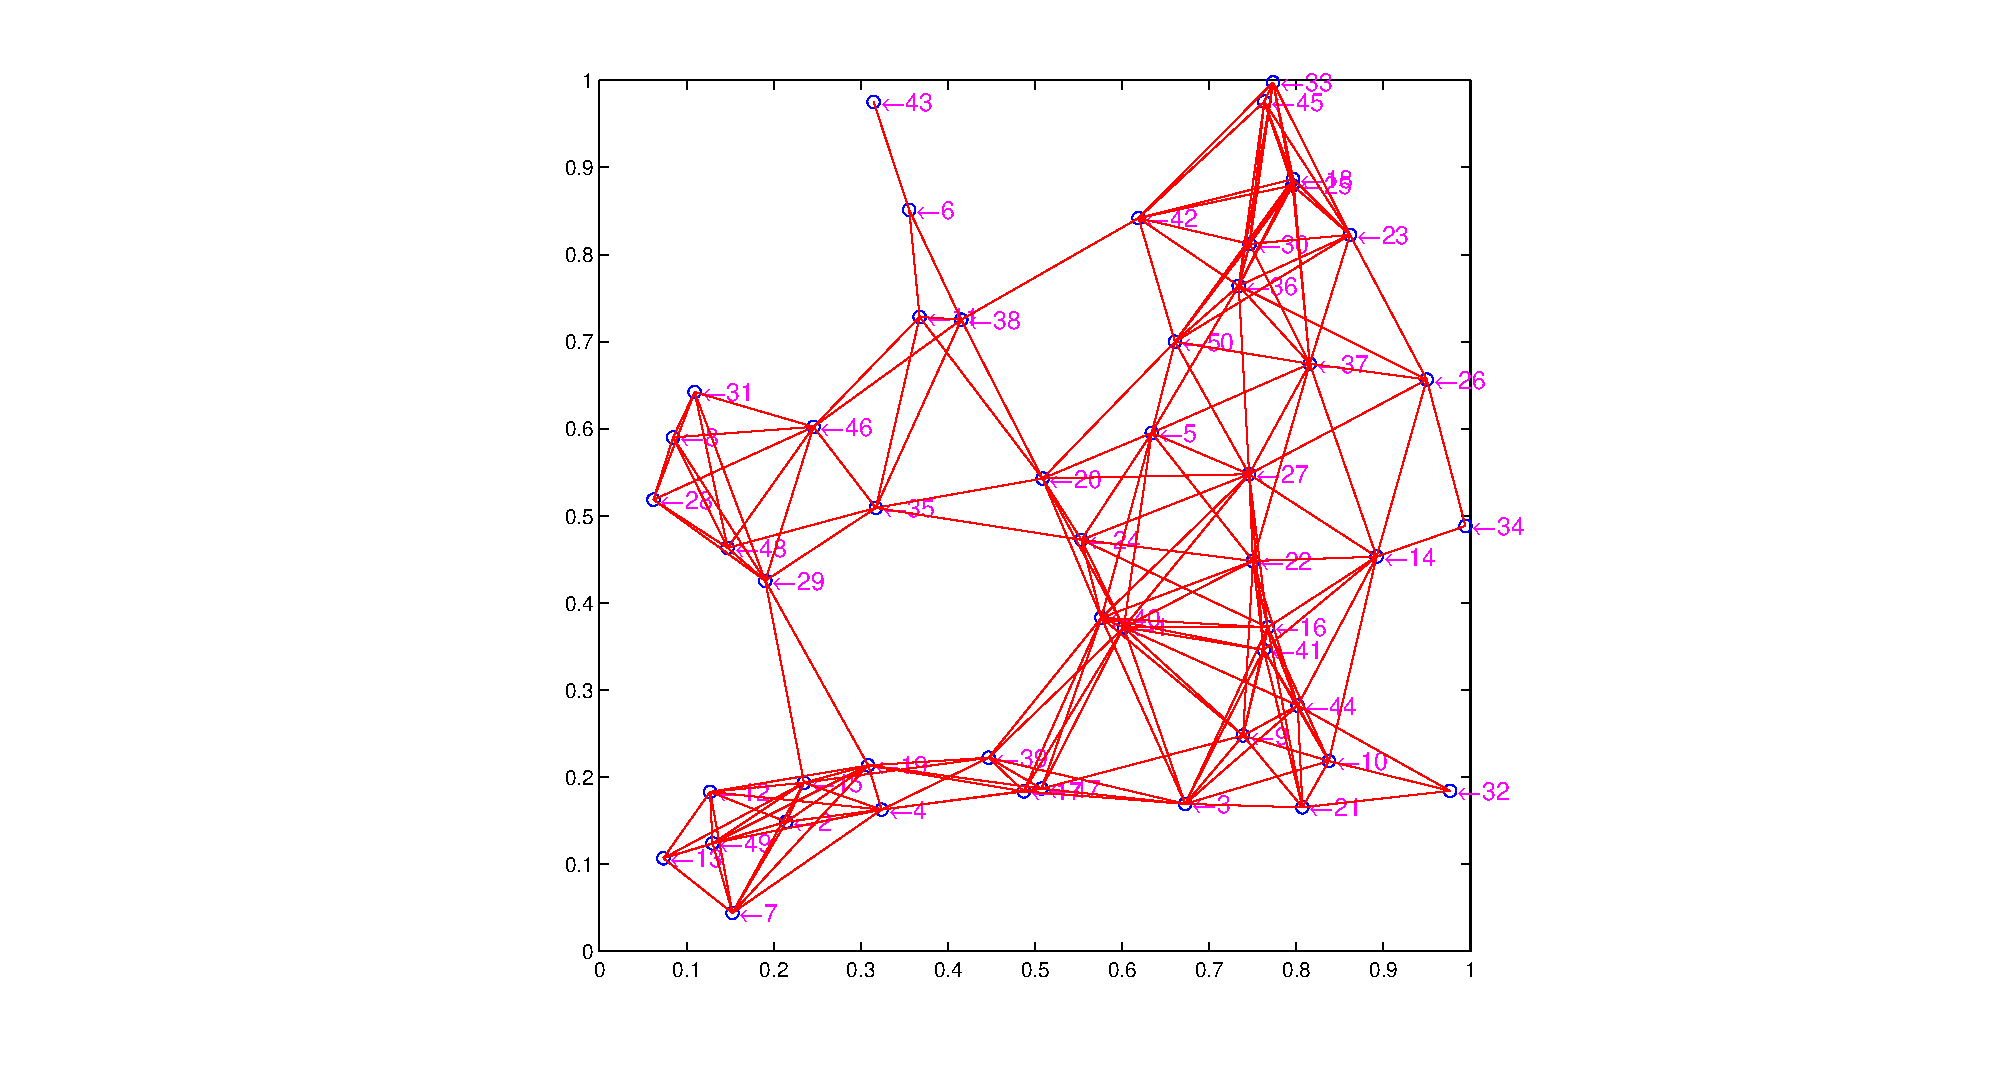
\includegraphics[width=7cm]{Graph/FirstYearReport/Lyx_v/images/Net50Edges200}

}\hfill{}\subfloat[\label{fig:Net-N16-R0,3}]{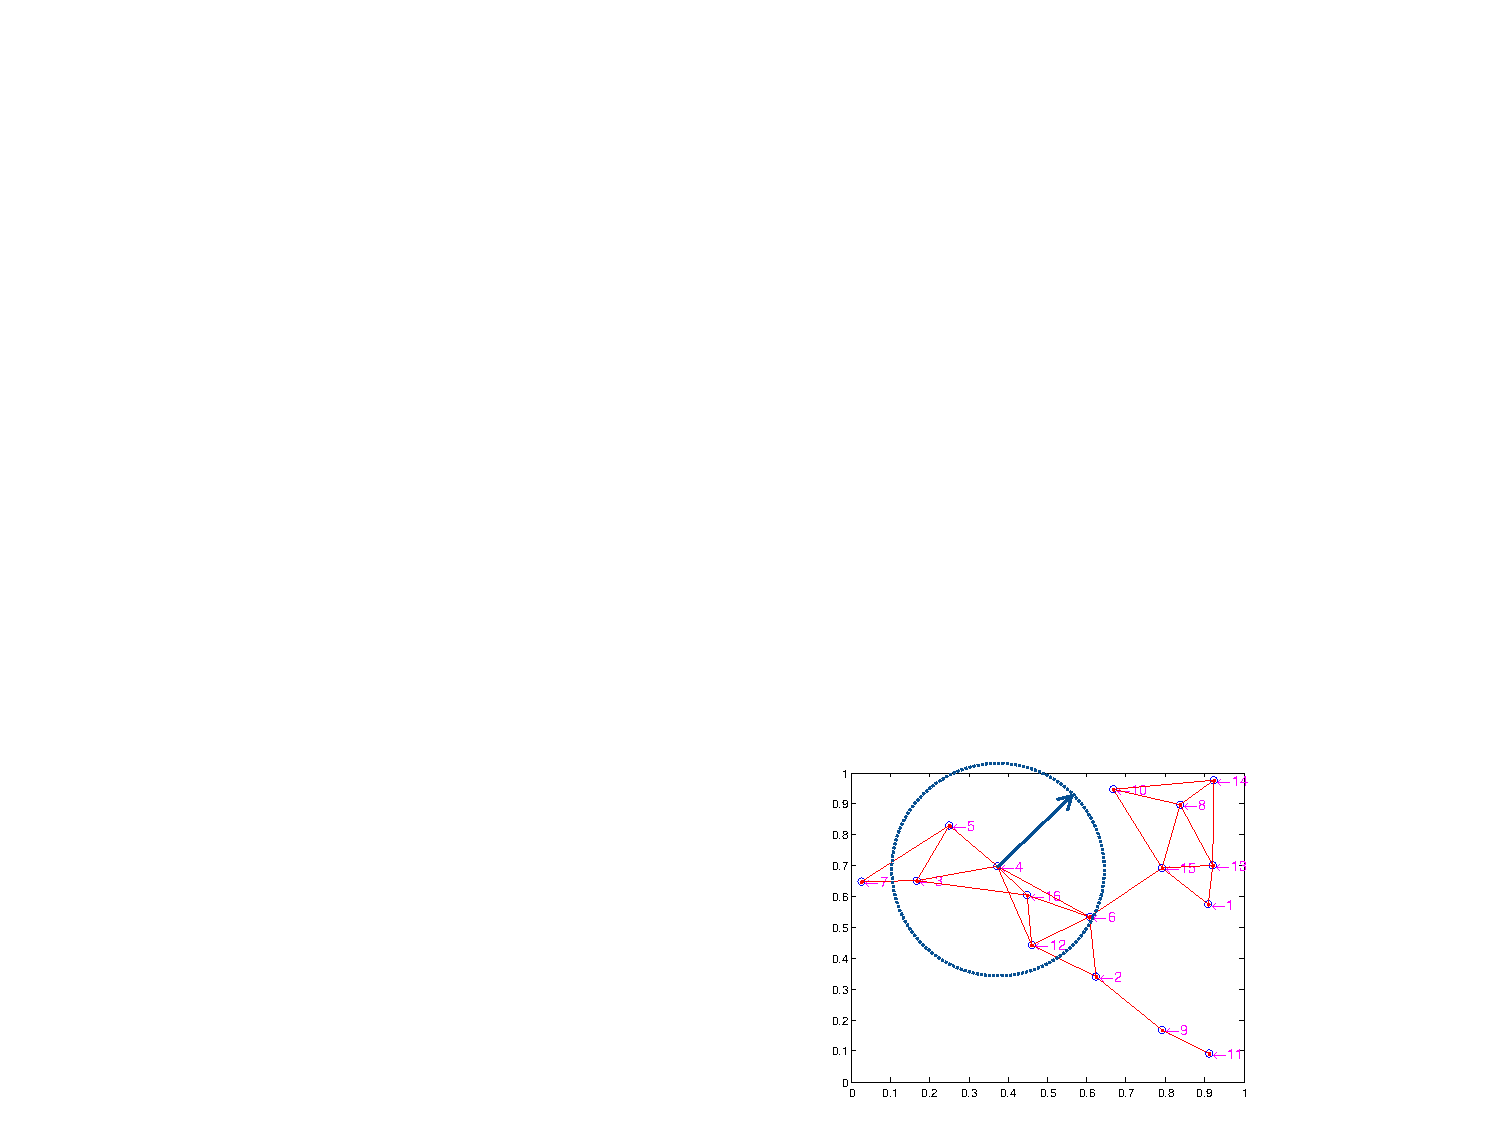
\includegraphics[width=7cm]{Graph/FirstYearReport/Lyx_v/images/Network_N16_R0,3}

}\hfill{}\caption{\label{fig:Random-Network}Randomly generated networks (a) 50 nodes
and 200 edges (b) 16 nodes and radius constrain $R=0.3$}
\end{figure}


There are some cases to generate the links between nodes.
\begin{casenv}
\item Consider the graph show in the Fig.\ref{fig:Net-N50-E200}, which
has 50 nodes and 200 edges.The number of nodes and edges are fixed;
50 nodes are randomly and uniformly distribute in the unit square;
a list that contains 200 shortest edges is created; Nodes are connected
if the edges belongs to the list. 
\item The network in Fig.\ref{fig:Net-N16-R0,3} is generating by connecting
any two nodes if their distance is less than the communication radius
constrain $R$. 
\end{casenv}

\subsubsection{Performance Comparison for Asymptotic DAC}

The figure.\ref{fig:DAC-SR-comp} shows the optimal spectral radius
for DAC algorithms with different communication radius constraints.
The performance for DAC algorithms with different orders are compared
by optimal spectral radius $\rho_{opt}=\mbox{\mbox{min}}\rho\left\{ \left(\mathbf{H}-\mathbf{J}\right)\right\} $,
which has the relationship with convergence rate given by $r_{opt}=-log\left(\rho_{opt}\right)$.
Y-axis is corresponding to the minimum spectral radius and x-axis
is corresponding to the radius constrain. For each instance of DAC
algorithm, the result is the minimum on the surface $\mbox{max}\{\left|\lambda_{i}\left(\mathbf{H-J}\right)\right|\}$
obtained by numerical searching. Each curve is the average of simulations
realized for 1000 instance of DAC initialized with random local value
vectors and random networks.

In another point of view, figure.\ref{fig:DAC MSE Compare} plots
the convergence behavior of mean square error of high-order DAC algorithms
together with first order DAC on random network. The MSE is defined
by 
\begin{equation}
MSE(k)=\frac{1}{n}\sum_{i=1}^{n}\left|x_{i}(k)-\bar{x}\right|^{2}.
\end{equation}
which Actually it is the Euclidean distance between current local
vector and the global average. shows the result when radius constrain
$R$ is $0.3$. In observing the gradient of curves, it is apparent
that higher-order DAC algorithm have larger convergence rate. However,
there are negligible improvement for the fourth order DAC compared
to the third order one. Furthermore, high-order DAC has a MSE overshoot
at the beginning. This phenomenon happens especially when communication
radius is small. Second order DAC algorithm does have a faster convergence
rate than first order algorithm as the slop of the curve is steeper.
But it become worse as it converge to error tolerance $10^{-6}$ more
later than the first order algorithm. Therefore, A hybrid algorithm
is proposed to overcome this disadvantage. Its step size and forgetting
factor are equal to the of first order DAC step size and second order
DAC forgetting factor respectively.

\begin{figure}
\hfill{}\subfloat[\label{fig:DAC-SR-comp} ]{\includegraphics[width=7cm,height=6.5cm]{\string"Graph/FirstYearReport/Lyx_v/images/Spectrum radius Compare_old_Ord1234\string".pdf}}\hfill{}\subfloat[\label{fig:DAC MSE Compare} ]{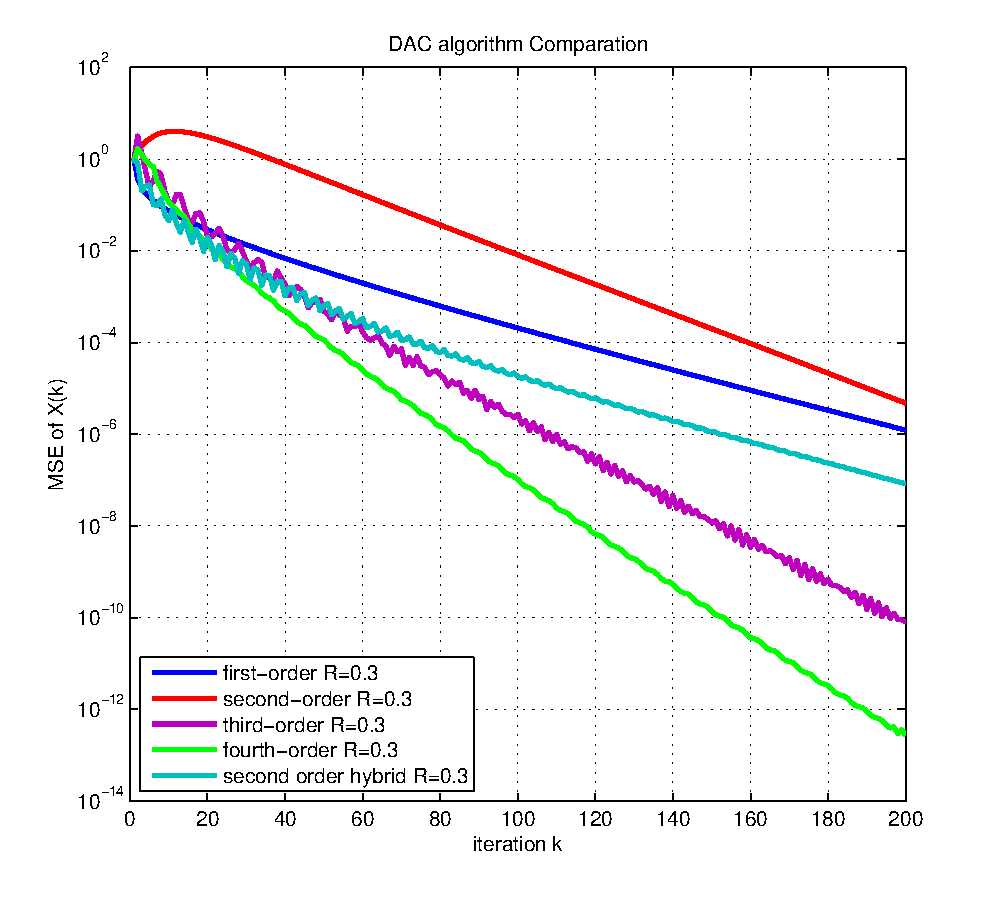
\includegraphics[width=7cm,height=6.5cm]{Graph/FirstYearReport/Lyx_v/images/DAC_Compr_ord1234&hybrid}

}\hfill{}

\caption{\label{fig:DAC-comparation}DAC algorithms comparison (a) compared
by spectral radius (b) compared by MSE}
\end{figure}




\section{\label{sec:Finite-Time-Distributed-Consensu}Finite-Time Distributed
Consensus Algorithm}

Finite-Time Distributed Consensus Algorithm (FT-DCA) is an non-asymptotic
algorithm. It tries to find the consensus value after each node run
the FO-DCA algorithm iteratively for a certain number of time. This
is based on the assumption that after a certain number of iterations,
local values would contain sufficient information to estimate the
consensus value.  
\begin{defn}
Given the network $\mathcal{G}$, and initial local value vector $\mathbf{x}\left(0\right)$,
it is said the algorithm achieves a finite-time consensus if it solves
a consensus problem, and there exist a time $t^{*}$ and the consensus
value $\bar{x}$ such that $x_{i}\left(t\right)=\bar{x}$, for all
time $t>t^{*}$. 
\end{defn}
Motivated by the works in \cite{Kokiopoulou2007}, we try to decompose
the local value vector in a form which reveals an important property
of its iteration. Therefore we propose a filtering technique to estimate
the consensus value. 


\subsection{\label{sub:Find_Consensus_Value}Find the Consensus Value by Linear
Filter}

In the network that adopts first order linear consensus algorithm,
each node has a number of consecutive local values obtained by Eq.\prettyref{eq:1st iter. ni}.
There exists a linear filter. If each node passes its consecutive
local values through this filter, the output after a certain time
is the global average of the initial values over the network. Compared
to first order DCA algorithm, no more information exchanged between
nodes is needed. Such a filter is defined as the \textit{consensus
finding filter}. 
\begin{thm}
\label{thm.A-consensus-finding}There exists a linear filter defined
by $\mathbf{h}\in R^{d}$, such that by passing through local values
\textup{$x_{i}(k)$} \textup{obtained by Eq.\prettyref{eq:1st iter. ni},
}the output \textup{$\hat{x}_{i}(k)=\mathbf{h}(k)*x_{i}(k)$} is the
consensus value \textup{$\overline{x}=\frac{1}{n}\sum_{i=1}^{n}x_{i}(0)$}
of the network after $k$ step $\left(k\geqslant m\right)$, where
\textup{$m$ is the number of} distinct and nonzero eigenvalues of
the weight matrix $W$ and $W$ satisfies the convergence condition\textup{
\ref{eq:convege condition W}. }\end{thm}
\begin{proof}
To avoid complicate analysis, suppose an undirected network with $n$
nodes, where duplex communication is possible in each link. Therefore,
the associated weight matrix $W\in\mathbf{R}^{n\times n}$ is symmetric
and diagonalizable. W Thus, there are $n$ linear independent eigenvectors
of the weight matrix. Let $\mathbf{e}_{1},\mathbf{e}_{2},\ldots,\mathbf{e}_{n}$
be the eigenvectors of $W$ and $\lambda_{1},\lambda_{2},\ldots,\lambda_{n}$
be the associated eigenvalues. They are ordered so that $1=\left|\lambda_{1}\right|\geq\left|\lambda_{2}\right|\geq\ldots\geq\left|\lambda_{n}\right|$.
$\lambda_{1}$ is called the dominant eigenvalue and $\mathbf{e}_{1}$
is associated dominant eigenvector.Since all the eigenvectors consist
a basis of $\mathbf{R}^{n}$, any initial value vector can be written
in a linear combination of these eigenvectors, 

\begin{equation}
\mathbf{x}\left(0\right)=\alpha_{1}\mathbf{e}_{1}+\alpha_{2}\mathbf{e}_{2}+\ldots+\alpha_{n}\mathbf{e}_{n}
\end{equation}
where $\alpha_{i}(i=1,2,\ldots,n)$ is the coefficient. For $k=1,2,3,...$
we have

\begin{eqnarray}
\mathbf{x}\left(k\right) & = & W^{k}\left[\alpha_{1}\mathbf{e}_{1}+\alpha_{2}\mathbf{e}_{2}+\ldots+\alpha_{n}\mathbf{e}_{n}\right]\nonumber \\
 & = & \alpha_{1}\lambda_{1}^{k}\mathbf{e}_{1}+\alpha_{2}\lambda_{2}^{k}\mathbf{e}_{2}+\ldots+\alpha_{n}\lambda_{n}^{k}\mathbf{e}_{n}\label{eq:x(k) decomposition}\\
 & = & \sum_{i=1}^{n}\alpha_{i}\lambda_{i}^{k}\mathbf{e}_{i}\nonumber 
\end{eqnarray}
where $\lambda_{i}$ is the eigenvalue of $W$. 

By rewriting $\mathbf{x}\left(k\right)$, it is clear that if all
eigenvalues of the weight matrix are known, the node values vector
is predictable and the consensus value can be found. For any node
$i=1,2,\ldots n$, its local value at time $k$ can be written as
\begin{equation}
x_{i}\left(k\right)=\alpha_{1}\lambda_{1}^{k}e_{i1}+\alpha_{2}\lambda_{2}^{k}e_{i2}+\ldots+\alpha_{n}\lambda_{n}^{k}e_{in}
\end{equation}
where $e_{ij}$ is the $i^{th}$ component of eigenvector $\mathbf{e}_{j}$.
Because of algebraic multiplicity of some eigenvalues, the equation
can be modified by combining the terms with the same eigenvalues.
Zero eigenvalues are ignored as they have no contribution in this
equation. Suppose $W$ has $m$ distinct and nonzero eigenvalues,
denoted by $\lambda_{1},\lambda_{2},\ldots,\lambda_{m}$, then $x_{i}\left(k\right)$
evolves into 
\begin{equation}
x_{i}\left(k\right)=\beta_{i1}\lambda_{1}^{k}+\beta_{i2}\lambda_{2}^{k}+\ldots+\beta_{im}\lambda_{m}^{k}
\end{equation}
where $\beta_{ij}$ is the coefficient after combination. 

Let the sample vector $\mathbf{y}_{i}(k,d)\in R^{d}$ is defined by
the history of $x_{i}(k),$ 

\begin{equation}
\mathbf{y}_{i}(k,d)=\left[x_{i}(k),x_{i}(k+1),\ldots x_{i}(k+d-1)\right]^{\mathrm{T}}\label{eq:def. y(k,m)}
\end{equation}
and the Vandermonde matrix whose entries are the power of eigenvalues

\begin{equation}
\mathbf{V}(k,d)=\left[\begin{array}{cccc}
\lambda_{1}^{k} & \lambda_{2}^{k} & \cdots & \lambda_{m}^{k}\\
\lambda_{1}^{k+1} & \lambda_{2}^{k+1} & \cdots & \lambda_{m}^{k+1}\\
\vdots & \vdots & \ddots & \vdots\\
\lambda_{1}^{k+d-1} & \lambda_{2}^{k+d-1} & \cdots & \lambda_{m}^{k+d-1}
\end{array}\right]\label{eq:def. Lamda(k,m)}
\end{equation}
and $\mathbf{b}_{i}\left(d\right)=\left[\beta_{i1},\beta_{i2},\cdots\beta_{id}\right]^{\mathrm{T}}$,
then we have the following equation satisfied

\begin{equation}
\mathbf{y}_{i}(k,d)=\mathbf{V}(k,d)\mathbf{b}_{i}\left(d\right)\label{eq:Vander_beta}
\end{equation}
To obtain the consensus value $\bar{x}$ for node $i$, we need to
take sufficient samples of $x_{i}(k)$\textbf{ }and solve Eq.\prettyref{eq:Vander_beta},
where $d$ should at least equal or larger than\textbf{ $m$}, which
is the number of distinct and nonzero eigenvalues of weight matrix
$W$

Let $A(k,m)=\mathbf{V}^{-1}(k,m)$ and the first row of $A(k,m)$
is given by 
\begin{equation}
\mathbf{h}=\left[A_{11}(k,m),A_{12}(k,m),\ldots,A_{1m}(k,m)\right]^{\mathrm{T}}
\end{equation}
 we have 

\begin{equation}
\beta_{i1}=\mathbf{h}^{\mathrm{T}}\mathbf{y}_{i}(k,m)\label{eq:Find Consensus m order}
\end{equation}
 Eq.\prettyref{eq:Find Consensus m order} shows that the consensus
value can be calculated by the filter defined in Def.\ref{thm.A-consensus-finding}.
This ends the proof.
\end{proof}
It is worth noting that Vandermonde matrix is related to a polynomial
interpolation problem and can be easily inverted in terms of Lagrange
basis polynomials \cite{Prass2007}. Due to this reason, this method
can be treated as an extrapolation method which find the consensus
value at infinity. At the same time, we only need to find out the
first coefficient $\beta_{i1}$ in the distributed averaging. Therefore,
only the elements in the corresponding row of $\mathbf{V}^{-1}(k,m)$
need to be found. This approach can save lots of computation time
in the inverting of Vandermonde matrix. 

Since simulation result shows that $\mathbf{h}$ is only depends the
associated Vandermonde matrix $\mathbf{V}(k,m)$ which is independent
of the nodes initial values and time index $k$. Therefore, each node
in the network could find the consensus value at any time $k\geqslant m$
by passing a number of consecutive local values through this filter.
In addition, all nodes in this network may share the same filter,
which means all the filters have the same impulse response. However,
such a consensus finding filter it is not unique. As an example, a
number of filters which have different impulse response or filter
lengths are found by different samples of $x_{i}(k)$.  Each node
could choose its own, but filter length determines the how many time-steps
before a node could find the consensus value. 

Suppose we take $d$ samples of $x_{i}(k)$, where $d>m$. Because
the Vandermonde matrix $\mathbf{V}(k,d)\in R^{d\times m}$ is non-square,
we introduce the Moore-Penrose pseudo inverse to find the least mean
square solution. 

Let

\begin{equation}
A(k,d)=\mathbf{V}^{+}(k,d)
\end{equation}
where $^{+}$ denote the Moore-Penrose pseudo inverse \cite{Piziak2007}.
And the first row of $A(k,d)$ is given by 

\begin{equation}
\mathbf{h}'=\left[A{}_{11}(k,d),A_{12}(k,d),\ldots,A_{1d}(k,d)\right]^{\mathrm{T}}
\end{equation}
Still, the value $\beta_{i1}=\mathbf{h}'^{\mathrm{T}}\mathbf{y}_{i}(k,m)$
is an accurate estimation of consensus value. Therefore, another consensus
finding filter is obtained.

Due to the multiplication of the consensus finding filter, the set
of filter is defined by

\begin{equation}
\{\mathbf{h}\in R^{d}|\forall d\geqslant m,\:\mathbf{h}^{\mathrm{T}}\mathbf{y}_{i}(k,d)=\bar{x}\}
\end{equation}
However, the shortest filter has its length equal to $m$, which means
node can only have the consensus value after $m$ steps. 

In \prettyref{sub:Numerical-Simulation}, the performance of this
algorithm is shown by comparing it with the first order DAC algorithm
using optimal weight matrix in \cite{Xiao2004}.


\subsection{Inverse the Vandermonde matrix}

The Vandermonde matrix has its application in some problems like polynomial
fitting, reconstruction of distributions from their moments, and so
on. Solving Vandermonde matrix is related to a polynomial interpolation
problem and can be easily inverted in terms of Lagrange basis polynomials.
It can be very difficult to invert in other way if the size of the
matrix is large, as the Vandermonde matrix is notoriously ill-conditioned
by its nature. It is a good way to always work on the problems related
to Vandermonde matrix in double precision or higher. 

Let $V_{m}$ be the Vandermonde's matrix of order $m$ given by 

\begin{equation}
V_{m}=\left[\begin{array}{cccc}
\lambda_{1} & \lambda_{2} & \cdots & \lambda_{m}\\
\lambda_{1}^{2} & \lambda_{2}^{2} & \cdots & \lambda_{m}^{2}\\
\vdots & \vdots & \ddots & \vdots\\
\lambda_{1}^{m} & \lambda_{2}^{m} & \cdots & \lambda_{m}^{m}
\end{array}\right]\label{eq:Vander Matrix}
\end{equation}
Then the equation 
\begin{equation}
\left[\begin{array}{cccc}
\lambda_{1} & \lambda_{2} & \cdots & \lambda_{m}\\
\lambda_{1}^{2} & \lambda_{2}^{2} & \cdots & \lambda_{m}^{2}\\
\vdots & \vdots & \ddots & \vdots\\
\lambda_{1}^{m} & \lambda_{2}^{m} & \cdots & \lambda_{m}^{m}
\end{array}\right]\left[\begin{array}{c}
\beta_{1}\\
\beta_{2}\\
\vdots\\
\beta_{m}
\end{array}\right]=\left[\begin{array}{c}
y_{1}\\
y_{2}\\
\vdots\\
y_{m}
\end{array}\right]\label{eq:Vander Eq.}
\end{equation}
is related to the problem of moments: Given the values of all $\lambda_{i}$,
find the unknown coefficients $b_{i}$, so that they match the given
values $y_{i}$ of the first $m$ moments. 

Its inverse is closely related to Lagrange's polynomial interpolation
formula. 

Let the polynomial of degree $m$ defined by 
\begin{equation}
P_{j}\left(\lambda\right)=\prod_{\begin{array}{c}
i=1\\
i\neq j
\end{array}}^{m}\frac{\lambda-\lambda_{i}}{\lambda_{j}-\lambda_{i}}=\sum_{k=1}^{m}b_{jk}\lambda^{k-1}\label{eq:Lagrange's polynomial}
\end{equation}
The polynomial $P_{j}\left(\lambda\right)$ a function of $\lambda$
and is specially designed so that it is equal to zero at all $\lambda_{i}$
except $i=j$ and takes on a value of one at $\lambda=\lambda_{j}$.
In other words, 
\[
P_{j}\left(\lambda_{i}\right)=\delta_{ij}=\sum_{k=1}^{m}b_{jk}\lambda_{i}^{k-1}
\]
where $\delta_{ij}=1$ when $i=j$. The equation says that $b_{jk}$
is exactly the inverse of the matrix \prettyref{eq:Vander Matrix},
with the subscript $k$ as the column index. 

To drive the analytical expression of $b_{jk}$ and make it as easy
as possible, let's define some intermediate result. Define the polynomial
$q_{j}\left(\lambda\right)$ and work out its coefficients

\begin{eqnarray}
q_{j}\left(\lambda\right) & = & \frac{\prod_{i=1}^{m}\left(\lambda-\lambda_{i}\right)}{\left(\lambda-\lambda_{j}\right)}=\prod_{i=1,i\neq j}^{m}\left(\lambda-\lambda_{i}\right)\label{eq:intermindia polynomial}\\
 & = & c_{j,m}\lambda^{m-1}+c_{j,m-1}\lambda^{m-2}+\ldots+c_{j,2}\lambda+c_{j,1}\nonumber 
\end{eqnarray}
Examining the polynomial \ref{eq:Lagrange's polynomial} and polynomial
\ref{eq:intermindia polynomial}, we have 
\begin{eqnarray*}
b_{jk} & = & \frac{c_{j,m}}{q_{j}\left(\lambda_{j}\right)}
\end{eqnarray*}
Therefore, the solution of Eq.\prettyref{eq:Vander Eq.} is just the inverse
of Vandermonde matrix time the vector on the right. 
\[
\beta_{j}=\sum_{k=1}^{m}b_{jk}y_{k}
\]
If we only need to calculate the consensus value, as explained in
\ref{sub:Find_Consensus_Value} only the elements in the corresponding
row of inverse Vandermonde's matrix need to be found. The computation
saving can be enormous by this approach.



\section{Consensus Based Signal Processing}

Sensor networks have a variety of applications such as surveillance,
environment monitoring and collaborative signal processing. As the
advatages of reliability, survivability, and increased range of coverage,
there is an increasing interest in employing multiple distributed
sensors for these applications \cite{Chair1986}. A fundamental problem
in sensor network is to process spatially distributed information
using a scalable algorithm \cite{Olfati-Saber2005a}. 

Generally, there are two options for multiple sensors signal processing:
First option is centralized signal processing. This requires the network
contains a fusion center, and all sensor's information being transmuted
to the central processor. 

The Second option is distributed signal processing. Distributed average
consensus (DAC) algorithm is a tool for distributed information processing.
It has received significant attention recently because of its robustness
and simplicity. In this section, we will introduce two distributed
signal processing methods based on consensus algorithm.


\subsection{Data Fusion and Decision Making}

In this section, we will consider a distributed detection problem
in wireless sensor network without the fusion center. A consensus
based approach of distributed data fusion and decision making is introduced.

In centralized data fusion and decision making, a hypothesis test
based on the ML, MAP or Bayesian decision rule will be carried out
at the a fusion center.  Therefore, we intend to carry out the hypothesis
test in a distributed manner. 

Considering a binary hypothesis testing problem with the following
two hypotheses
\begin{enumerate}
\item H0: target is absent
\item H1: target is present.
\end{enumerate}
Suppose each sensor acquires a scale value from its sensoring area,
its signal has the following form

\begin{equation}
x_{l}=\begin{cases}
\mu_{l,0}+n_{l} & \mbox{if no target presents}\\
\mu_{l,1}+n_{l} & \mbox{if target presents}
\end{cases}
\end{equation}
where $\mu_{l,m}$ is the mean value of $x_{l}$ depending on hypothesis
$m$ and $n_{l}$ is the noise of $x_{l}$. The prior probability
of these two hypotheses is denoted by $P\left(H_{m}\right)=P_{m},m=1,2$.
The case when each sensor acquires a vector of unknown parameters
is discussed in \cite{Xiao2005}, where a more sophisticated data
fusion scheme is proposed.   

To make a declaration whether the target presents or not, based on
classical hypothesis test theory, the global log likelihood ratio
(G-LLR ) test is given by 

\begin{equation}
LLR(x_{1},...,x_{L})=\log\frac{f\left(x_{1},...,x_{L}|H_{1}\right)}{f\left(x_{1},...,x_{L}|H_{0}\right)}\underset{H_{0}}{\overset{H_{1}}{\gtrless}\log}\frac{P\left(H_{o}\right)}{P\left(H_{1}\right)}\label{eq:G-LLR define}
\end{equation}
where $f\left(x_{1},...,x_{L}|H_{m}\right)$ is the likelihood function
of hypothesis $H_{m}$.

Usually  we can assume the sensor detections are independent from
one to another. Therefore, we have $f\left(x_{1},...,x_{L}|H_{m}\right)=f\left(x_{1}|H_{1}\right)\cdot\ldots\cdot f\left(x_{L}|H_{1}\right)$
and 

\begin{eqnarray}
LLR(\mathbf{x}) & = & \log\frac{f\left(x_{1}|H_{1}\right)\cdot\ldots\cdot f\left(x_{L}|H_{1}\right)}{f\left(x_{1}|H_{0}\right)\cdot\ldots\cdot f\left(x_{L}|H_{0}\right)}=\sum_{i=1}^{L}LLR\left(x_{i}\right)\label{eq:Sum_L_LLR}
\end{eqnarray}


According to Eq.\prettyref{eq:Sum_L_LLR}, the G-LLR is the sum of local
log likelihood ratio (L-LLR) and can be calculated by distributed
average consensus (DAC) algorithm. This is implemented by the following
steps: First, each sensor node $i$ only calculate its L-LLR individually
based on $x_{i}$; Then, all the sensors update their L-LLR in the
DAC iteration until they converge to a common value; Finally, once
the algorithm converges, the G-LLR is obtained by multiply the average
value with the number of sensors in the network.


\subsubsection*{Generalization of LLR Calculation }

In this section, we will generalize the conditions step by step and
drive some expressions to show how to calculate G-LLR with DAC algorithms. 

First we assume the noises in sensor's signals are not independent
from one to another. The noises can be denoted by the joint Gaussian
white noise. 

Let the sensors observation, the joint Gaussian white noises and the
mean of sensor observation in a vector form given by 
\[
\mathbf{x}=\left[x_{1},\ldots,x_{L}\right]^{\mathrm{T}}
\]


\[
\mathbf{n}=\left[n_{1},\ldots,n_{L}\right]^{\mathrm{T}}\sim\mathcal{N}\left(0,\Sigma\right)
\]


\begin{equation}
\mathbf{u}_{m}=\left[\mu_{1,m},\ldots,\mu_{L,m}\right]^{\mathrm{T}},\; m=0,1.
\end{equation}
Since $\mathbf{n}\sim\mathcal{N}\left(0,\Sigma\right)$, the likelihood
function is a joint Gaussian function $f\left(x_{1},...,x_{L}|H_{m}\right)=\frac{1}{\left(2\pi\right)^{L/2}\left|\Sigma\right|^{\frac{1}{2}}}\exp\left(-\frac{1}{2}\left(\mathbf{x}-\mathbf{u}_{m}\right)^{T}\Sigma^{-1}\left(\mathbf{x}-\mathbf{u}_{m}\right)\right)$,
the G-LLR becomes 
\begin{eqnarray}
LLR(\mathbf{x}) & = & \left(\mathbf{u}_{1}^{\mathrm{T}}-\mathbf{u}_{0}^{\mathrm{T}}\right)\mathbf{\Sigma}^{-1}\mathbf{x}+\frac{1}{2}\left(\mathbf{u}_{0}^{\mathrm{T}}\mathbf{\Sigma}^{-1}\mathbf{u}_{0}-\mathbf{u}_{1}^{\mathrm{T}}\mathbf{\Sigma}^{-1}\mathbf{u}_{1}\right)\label{eq:wighted_sum_LLR}\\
 & = & \sum_{l=1}^{L}w_{l}x_{l}+C\nonumber 
\end{eqnarray}
where $w_{l}$ is the $l^{th}$ component of $\left(\mathbf{u}_{1}^{\mathrm{T}}-\mathbf{u}_{0}^{\mathrm{T}}\right)\mathbf{\Sigma}^{-1}$,
$C$ is the last term the equation. Eq.\ref{eq:wighted_sum_LLR}\prettyref{wighted_sum_LLR} means
 the G-LLR can be a weighted sum of sensor's observation. 

Provided that each sensor knows the weight $w_{l}$ and $C$, the
G-LLR is equal to the weighted sum of sensor's observation plus $C$.
Actually, the constant $C$ changes the threshold of the hypothesis
testing and can be subtract from both side of the equation. Therefore,
we modify the hypothesis testing into 
\[
\sum_{l=1}^{L}w_{l}x_{l}\underset{H_{0}}{\overset{H_{1}}{\gtrless}}\frac{P\left(H_{o}\right)}{P\left(H_{1}\right)}-C
\]
where the average values $\mbox{Avg}\left(w_{l}x_{l}\right)$ is obtained
by distributed average consensus (DAC) algorithm. Then the average
is multiplied with the number of sensors in the network to get $\sum_{l=1}^{L}w_{l}x_{l}$.


In the section of cloud detection \secref{Distributed_Cloud_De},
more generalized conditions of calculating the G-LLR is discussed
and more results about applying DAC algorithm will be presented. The
sensor signals will be correlated and mixed with joint Gaussian white
noises. In addition, the noises are not only correlated but also depends
on the existence of target. 


\subsection{Network Information Flooding}

The conventional information flooding is actually done by copying
information to all other nodes. Each node maintains a table of the
of all nodes values in the network, initialized with its own value,
and exchanges the tables of their own with those from their neighbors
in each step. After a certain number of time steps which is equal
to the diameter of the network, each node will obtain values of all
nodes. distributed averaging can also be implemented by this way. 

However, copying information and forwarding to all other nodes takes
too much resources for the networks. If a networks has $n$ nodes,
the conventional flooding will needs at least $\left(n-1\right)$
copies for each piece of information. And this estimation doesn't
considering the cost in transmitting the information to the destination.

We intend to develop an algorithm to accomplish the information flooding,
but didn't copy all the information to other nodes, so that the communication
cost can be dramatically reduced. However, The difficulties of this
kinds of distributed signal processing is that any individual node
only know partial information on the whole network. And information
exchange only allowed between neighbors. 

Based on the FT-DAC algorithm we introduced in the section \ref{sub:Finite-time-Consensus-on},
each node could decompose the local value vector by a linear combination
of eigenvalues and eigenvectors and can calculate the coefficients
before each term. Actually, with some signal processing techniques,
there are more information in the local values sequence that each
node can extract. These may also be applied to wireless sensor networks
as they could be carried out distributively. 

Therefore, in this section we propose a novel network information
flooding technique based on consensus algorithm. It doesn't require
copying information for so many time, instead, it transmit information
by broadcasting. The advantage of this method is that it can save
the costs in copying and transmitting information. 

Suppose the network weight matrix $W$ satisfies the same condition
\ref{eq:convege condition W}. Recall the initial local value decomposition
given by

\begin{equation}
\mathbf{x}\left(0\right)=\sum_{j=1}^{n}\alpha_{j}\mathbf{e}_{j}\label{eq:initial vector decompose-1}
\end{equation}
which shows that the initial local value vector can be defined by
a set of coefficients and a new basis defined by the eigenvectors.\textbf{
}In addition, the eigenvectors $\mathbf{e}_{i}$ are only depends
on the weight matrix. Therefore, once the coefficients $\alpha_{i}$
and weight matrix are available, the initial values vector $\mathbf{x}\left(0\right)$
can be calculated. It is possible to exchange information between
nodes in the network without copying information to all other nodes.

To show how this method can be carried out distributively, let the
sample vector $\mathbf{y}_{i}(k,d)\in R^{d}$ is defined by the history
of $x_{i}(k)$ 

\begin{equation}
\mathbf{y}_{i}(k,d)=\left[x_{i}(k),x_{i}(k-1),\ldots x_{i}(k-d+1)\right]^{\mathrm{T}}
\end{equation}
and the coefficients vector $\mathbf{a}=\left[\alpha_{1},\alpha_{2},\ldots,\alpha_{n}\right]^{T}$.
If we involve the eigenvectors and redefine the \eqref{Vander_beta}
by 
\begin{equation}
\mathbf{y}_{i}(k,d)=\mathbf{V}_{i}(k,d)diag\left(\left[\mathbf{e}_{1}^{T}\mathbf{u}_{i},\mathbf{e}_{2}^{T}\mathbf{u}_{i},\ldots,\mathbf{e}_{n}^{T}\mathbf{u}_{i}\right]\right)\mathbf{a}\label{eq:Vander_Eigen_ith_Alpha}
\end{equation}
where $\mathbf{u}_{i}$ is the unit vector with all zero except the
$i^{th}$ component is one, $\mathbf{e}_{j}^{T}\mathbf{u}_{i}$ means
the $i^{th}$ component of $\mathbf{e}_{j}$. Solving the above equation
will obtain the coefficients $\alpha_{j}$. 

The consensus based information flooding is ideally suitable for time-invariant
network. Because this method requires a node know all the eigenvectors
and eigenvalues of the network before it can estimate initial values
of other nodes. It can be initialized by all flooding weight coefficients
to all nodes in the network. However, instead of flooding a table
of local values, flooding the weight matrix is only performed at the
stage initialization for one time. The proposed method could have
lower cost both in computation and communication, if the topology
changes at a very low frequency.



\section{Graph Theory and Matrix Theory Review }

In this section, some basic concepts of the graph theory and matrix
theory will be introduced. They are used in the analysis of convergence
or performance of consensus algorithm. Because consensus algorithm
actually relates to a matrix iteration algorithm, it is necessary
to introduce some of these theorems. For full information about matrix
theory, see \cite{Varga2010}, and the work \cite{Russell1994} states
more details about Laplacian matrix. However, some useful properties
of Laplacian matrix will to be introduced here. 

Let ${\cal G}=\left({\cal V},{\cal E},{\cal A}\right)$ be a graph
with $n$ nodes. The in-degree and out-degree of node $i$ are defined
by:

\begin{equation}
D_{in}\left(i\right)=\sum_{i=1}^{n}a_{i,j}
\end{equation}
\begin{equation}
D_{out}\left(i\right)=\sum_{j=1}^{n}a_{i,j}
\end{equation}
where $a_{i,j}$ is the elements of matrix ${\cal A}$. This definition
states that in-degree of node $i$ is the $i^{th}$ column sum of
matrix ${\cal A}$ and the out-degree of node $i$ is the $i^{th}$
row sum of matrix ${\cal A}.$ And the graph Laplacian matrix ${\cal L}$
induced by the ${\cal G}$ is the same as defined before, see \ref{eq:Graph Laplacian def.}.
In addition, we can find the relationship of ${\cal L}$ and ${\cal A}$.
\begin{equation}
{\cal L}=\Delta-{\cal A}
\end{equation}
 where $\Delta$ is a diagonal matrix $\Delta=\left[\Delta_{i,j}\right]$,
$\Delta_{i,j}=0$ for all $i\neq j$ and $\Delta_{ii}=D_{out}\left(i\right)$.

Note that we assume the diagonal elements $a_{i,i}$ of matrix ${\cal A}$
equal to zero for all $i$. Thus, the Laplacian matrix is only dependent
on the off-diagonal elements of ${\cal A}$. Moreover, if we assume
matrix ${\cal A}$ is non-negative, we can benefit from the properties
of non-negative matrix, and use them in optimization of convergence
rate of consensus algorithm.


\subsection{Irreducibility and Strong Connected Graph.}

For an undirected graph, the consensus $\mathbf{x}^{*}$ can be achieved
if and only if the graph is connected. (Note that the consensus is
a stable state of the system dynamic. For the average consensus problem
the consensus state is a state where all the network node converge
to the global average.) But for the directed graph, this condition
of achieving consensus becomes into if and only if the graph is strongly
connected. 

A directed graph is strongly connected if and only if for any two
distinct nodes $i$ and $j$, there exists a path that follows the
direction of the edges and connects $i$ and $j$ on the digraph. 
\begin{defn}
\label{Def.Irreducebility}for $n>1$, an $n\times n$ matrix $A\in R^{n\times n}$
is reducible if there exists an $n\times n$ permutation matrix $P$
such that $PAP^{T}$ is in block upper triangular form. 
\begin{equation}
PAP^{T}=\left[\begin{array}{cc}
A_{1,1} & A_{1,2,}\\
O & A_{2,2}
\end{array}\right]
\end{equation}
where $A_{1,1}$ is an $r\times r$ submatrix and $A_{2,2}$ is an
$\left(n-r\right)\times\left(n-r\right)$ submatrix, and $O$ is an
null matrix, $1\leq r<n$. If no such a permutation matrix exists,
the matrix $A$ is irreducible. If $n=1$, then $A$ is reducible
if $A=0$, and irreducible otherwise. 
\end{defn}
The relationship of the irreducible property of matrix $A$ and the
strong connected property of directed graph ${\cal G}\left(A\right)$
is stated by the following theorem.
\begin{thm}
An $n\times n$ complex matrix $A\in C^{n\times n}$ is irreducible
if and only if its directed graph ${\cal G}\left(A\right)$ is strongly
connected. \cite{Varga2010}
\end{thm}
The proof of this theorem is obvious. If a graph is strongly connected,
all the off diagonal elements of graph matrix $A$ cannot be vanished
by matrix permutation. Therefore, matrix $A$ doesn't exists the block
upper triangular form as given in Def. \ref{Def.Irreducebility}. 


\subsection{Spectral radius of a matrix}

Spectral radius of a matrix is one of the basic concepts in the matrix
iteration theory. It is defined by the largest eigenvalue of the matrix.
The matrix iteration is very useful in many applications, denoted
by $A,A^{2},A^{3},\ldots$. The power sequence is said to be convergent,
if and only if $\lim_{k\to\infty}A^{k}=O$, where $O$ is a zero matrix
with all zero entries. The following theorem states that the convergent
property is strongly connected with the spectral radius. 
\begin{thm}
\label{thm:Convergent <=00003D> p(A)<1} if $A\in C^{n\times n}$
is an $n\times n$ complex matrix, then $A$ is convergent if and
only if $\rho\left(A\right)<1.$\end{thm}
\begin{proof}
The proof uses the Jordan form of a matrix. For any matrix $A\in C^{n\times n}$,
there exists a nonsingular $n\times n$ matrix $T$, such that $A$
reduces into the Jordan normal form 
\begin{equation}
T^{-1}AT=J=\left[\begin{array}{cccc}
J_{1} &  &  & O\\
 & J_{2}\\
O &  & \ddots & J_{m}
\end{array}\right]
\end{equation}
 where each Jordan block $J_{i}$ is an $r_{i}\times r_{i}$ submatrix
in the form 
\begin{equation}
J_{i}=\left[\begin{array}{ccccc}
\lambda_{i} & 1\\
 & \lambda_{i} & 1\\
 &  & \lambda_{i} & \ddots\\
 &  &  & \ddots & 1\\
 &  &  &  & \lambda_{i}
\end{array}\right]
\end{equation}
Thus, the matrix $J$ and $A$ are similar and have the same eigenvalues
$\lambda_{i},i=1,\ldots m$

A direct computation of the power iteration of matrix $A$ will give
us the following equation
\[
A^{k}=TJ^{k}T^{-1}=T\left[\begin{array}{cccc}
J_{1}^{k} &  &  & O\\
 & J_{2}^{k}\\
O &  & \ddots & J_{m}^{k}
\end{array}\right]T^{-1}
\]
because the property of Jordan block, the power of each Jordan block
will have the form
\[
J_{i}^{2}=\left[\begin{array}{ccccc}
\lambda_{i}^{2} & 2\lambda_{i} & 1\\
 & \lambda_{i}^{2} & 2\lambda_{i} & \ddots\\
 &  & \lambda_{i}^{2} & \ddots & 1\\
 &  &  & \ddots & 2\lambda_{i}\\
 &  &  &  & \lambda_{i}^{2}
\end{array}\right],\mbox{if }r_{i}\geq3
\]
 and more generally, let $J_{i}^{k}=\left[c_{m,n}\left(i,k\right)\right]$,
$1\leq m$, $n\leq r_{i}$, and it has 
\[
c_{m,n}\left(i,k\right)=\begin{cases}
0 & n<m\\
\left(\begin{array}{c}
k\\
n-m
\end{array}\right)\lambda_{i}^{k-n+m} & m\leq n\leq\min\left(r_{i},k+m\right)\\
0 & k+m<n<r_{i}
\end{cases}
\]
 Since $\rho\left(A\right)<1$, and matrix $J$ share the same eigenvalues
with $A$, $\left|\lambda_{i}\right|<1$. This lead to $\lim_{k\to\infty}c_{m,n}\left(i,k\right)=0,\:\mbox{for all }1\leq m\leq r_{i},1\leq n\leq r_{i}$,
so that the each Jordan block is convergent. Therefore, the matrix
iteration $A^{k}=TJ^{k}T^{-1}$ is also convergent. This completes
the proof. 
\end{proof}
We give the proof of \prettyref{thm:Convergent <=00003D> p(A)<1}
here as it will be very useful in the proof of an convergence conditions
theorem for distributed consensus algorithm, see \prettyref{sub:DT-First-Order-DAC}.
At the same time, the Jordan normal form weight matrix $W^{k}=TJ^{k}T^{-1}$
gives the local value vector $\mathbf{x}\left(k\right)=W^{k}\mathbf{x}\left(0\right)$
another expression in terms of eigenvalues and eigenvectors, which
reflects the basic ideas of the finite-time consensus algorithm. This
will be introduced in \prettyref{sec:Finite-Time-Distributed-Consensu}. 


\subsubsection{Gerschgorin's theorem}

The calculation of eigenvalues a matrix $A$ involves determination
of the matrix $\lambda I-A$ and solving a high order polynomial equation.
In some situations, for example, when the matrix dimension is very
large, it is very difficult to determine the spectral radius precisely.
However, the following theorem of Gerschgorin provides an upper bound
of the spectral radius \cite{Horn1990}.
\begin{thm}
Let $A=\left(a_{i,j}\right)$ be an arbitrary $n\times n$ matrix.
Denote the 
\begin{equation}
d_{i}=\sum_{j=1,j\neq i}^{n}\left|a_{i,j}\right|
\end{equation}
then all the eigenvalues of matrix $A$ are lie in the union of the
disks.
\begin{equation}
\left|z-a_{i,i}\right|\leq d_{i},\ 1\leq i\leq n.
\end{equation}

\end{thm}
The above theorem is well-known, so the proof is omit here. But the
theorem immediately give the result of
\begin{cor}
\label{cor:Upper Bound of p(A)}Let $A=\left(a_{i,j}\right)$ be an
arbitrary $n\times n$ matrix, and 
\begin{equation}
v=\max_{1\leq i\leq n}\sum_{j=1}^{n}\left|a_{i,j}\right|
\end{equation}
then we have $\rho\left(A\right)\leq v$. 
\end{cor}
Therefore, the maximum of the row sums of the modular of the entries
of matrix $A$ provides a upper bound for spectral radius $\rho\left(A\right)$.
Since $A$ and $A^{T}$ have the same eigenvalues, applying the \ref{cor:Upper Bound of p(A)}
to $A^{T}$ will lead to 
\begin{cor}
Let $A=\left(a_{i,j}\right)$ be an arbitrary $n\times n$ matrix,
and 
\begin{equation}
v'=\max_{1\leq j\leq n}\sum_{i=1}^{n}\left|a_{i,j}\right|
\end{equation}
then we have $\rho\left(A\right)\leq v'$.
\end{cor}
As both the row sum and column sum of the modular of the entries of
matrix can provide the upper bound for $\rho\left(A\right)$, the
minimum of $v$ and $v'$ gives the better upper bound. 



Just as we assume before, the adjacent matrix ${\cal A}$ of the graph
${\cal G}$ is non-negative, which means all elements are non-negative.
Then, the induced graph Laplacian matrix will have the following result
using the Gerschgorin's theorem. 




\subsubsection{Perron-Frobenius Theorem}

The Perron-Frobenius theorem states that if matrix $A$ is nonnegative
and irreducible which means the digraph of matrix A is strongly connected,
the spectral radius $\rho(A)$ is equal to a simple eigenvalue of
$A$ associated with a positive eigenvector \cite{Piziak2007}. The
details of Perron-Frobenius is as follows.
\begin{thm}
\label{thm:Perron-Frobenius thm.} Let $A$ be an $n\times n$ and
irreducible matrix with non-negative and real numbers as its entries.
Then, \end{thm}
\begin{enumerate}
\item $A$ has a positive real eigenvalue equal to its spectral radius $\rho\left(A\right)$.
\item $\rho\left(A\right)$ is a simple eigenvalue of $A$.
\item To the eigenvalue $\rho\left(A\right)$, the corresponding eigenvector
is positive, i.e. $\mathbf{x}>\mathbf{0}$.
\item $\rho\left(A\right)$ increases if any entry of $A$ increases.
\end{enumerate}
Recall the problem of finding the bounds for the spectral radius,
the Perron-Frobenius theorem provides the nontrivial lower-bound of
$\rho\left(A\right)$. In the \prettyref{cor:Upper Bound of p(A)},
the nontrivial upper bound of $\rho\left(A\right)$ is found. Together
with these two results, we can have a conclusion of the spectral radius
of a non-negative and irreducible matrix given in the following.
\begin{lem}
If $A=\left[a_{i,j}\right]$ is an $n\times n$ non-negative and irreducible
matrix, then either 
\begin{equation}
\sum_{j=1}^{n}a_{i,j}=\rho\left(A\right),\mbox{for all }1\leq i\leq n,
\end{equation}
or 
\begin{equation}
\min_{1\leq i\leq n}\left(\sum_{j=1}^{n}a_{i,j}\right)<\rho\left(A\right)<\max_{1\leq i\leq n}\left(\sum_{j=1}^{n}a_{i,j}\right).
\end{equation}
\end{lem}
\begin{thm}
Let $A=\left[a_{i,j}\right]$ be an $n\times n$ non-negative and
irreducible matrix, for any $\mathbf{x}>\mathbf{0}$, either
\begin{equation}
\min_{1\leq i\leq n}\left(\frac{\sum_{j=1}^{n}a_{i,j}x_{j}}{x_{i}}\right)<\rho\left(A\right)<\max_{1\leq i\leq n}\left(\frac{\sum_{j=1}^{n}a_{i,j}x_{j}}{x_{i}}\right)
\end{equation}
or 
\begin{equation}
\frac{\sum_{j=1}^{n}a_{i,j}x_{j}}{x_{i}}=\rho\left(A\right),\ \mbox{for all }1\leq i\leq n.
\end{equation}
Moreover,
\begin{equation}
\max_{\mathbf{x}\in P}\min_{1\leq i\leq n}\left(\frac{\sum_{j=1}^{n}a_{i,j}x_{j}}{x_{i}}\right)=\rho\left(A\right)=\min_{\mathbf{x}\in P}\max_{1\leq i\leq n}\left(\frac{\sum_{j=1}^{n}a_{i,j}x_{j}}{x_{i}}\right)
\end{equation}

\end{thm}
The equality is valid if we choose the $\mathbf{x}$ equal to the
positive eigenvector $e>0$ corresponding to the eigenvalue $\rho\left(A\right)$.
The method shown above will be applicable, because it provides us
both the upper bounds and lower bounds for the spectral radius of
a non-negative and irreducible matrix, by a simple algorithm without
calculating the determination of $\lambda I-A$. 




\subsection{Diagonalizable matrix \& Symmetric matrix}

The Jordan normal form of weight matrix $W^{k}=TJ^{k}T^{-1}$ gives
the local value vector $\mathbf{x}\left(k\right)=W^{k}\mathbf{x}\left(0\right)$
an analitical expression in terms of eigenvalues and eigenvectors.
Moreover, if the matrix $W$ is symmetric, the expressions of $\mathbf{x}\left(k\right)$
can be simplified. Then, algorithms such as the finite-time consensus,
can be implemented more easily. In addition, under the the assumption
of symmetric weight matrices, the optimal weight matrix which has
the fastest convergence rate can be found through a semi-definite
problem. \cite{Li2010}. 
\begin{defn}
A matrix $A$ is diagonalized, if and only if there exist a nonsigular
matrix $T$, which reduce $A$ into the form 
\[
T^{-1}AT=\mbox{diag}\left(\lambda_{1},\lambda_{2},\ldots,\lambda_{n}\right)
\]

\end{defn}
Generally, a matrix are diagonalized by an unitary matrix if and only
if it is normal. Normal matrix $A$ means it satisfies $A^{H}A=AA^{H}$.
Let $\lambda_{1},\lambda_{2},\ldots,\lambda_{n}$ be the eigenvalues
of $A$. There exists a unitary matrix $U$, which satisfies $U^{H}=U^{-1}$,
such that $U^{-1}AU=\mbox{diag}\left(\lambda_{1},\lambda_{2},\ldots,\lambda_{n}\right)$.
For real normal matrix $A$, if all of its eigenvalues are real, there
exists an orthogonal matrix $P,$ which has $P^{T}=P^{-1}$, reduces
the real matrix $A$ into diagonalized form $P^{-1}AP=\mbox{diag}\left(\lambda_{1},\lambda_{2},\ldots,\lambda_{n}\right)$. 

Specificlly, any real nonsigular symmetric matrix $A\in R^{n\times n}$
has $n$ linearly independent real eigenvectors. Moreover, these eigenvectors
can be chosen so that they are orthogonal to each other with modular
one. Thus, the real symmetric matrix can be decomposed by an orthogonal
matrix $P$, i.e. $A=P\Lambda P^{-1}$, where $\Lambda$ is a diagonal
matrix whose entries equal to the eigenvalues of $A$. Also the symmetric
matrix has all its eigenvalues algebra multiplicity equal to the gerometric
multiplicity, so all the Jordan block have size one.



\section{\label{sec:Finite-Time-Distributed-Consensu}Finite-Time Distributed
Consensus Algorithm}

Finite-Time Distributed Consensus Algorithm (FT-DCA) tries to find
the consensus value after each node run the FO-DCA algorithm iteratively
for a certain number of time. This is based on the assumption that
after a certain number of iterations, local values would contain sufficient
information to estimate the consensus value. (OK2.5)
\begin{defn}
Given the network $\mathcal{G}$, and initial local value vector $\mathbf{x}\left(0\right)$,
it is said the algorithm achieves a finite-time consensus if it solve
a consensus problem, and there exist a time $t^{*}$ and the consensus
value $\bar{x}$ such that $x_{i}\left(t\right)=\bar{x}$, for all
time $t>t^{*}$. 
\end{defn}
Motivated by the works in \cite{Kokiopoulou2007}, we try to decompose
the local value vector in a form which reveals an important property
of its iteration. Therefore we propose a filtering technique to estimate
the consensus value. (OK 3) 

In the network that adopts first order linear consensus algorithm,
each node has a number of consecutive local values obtained by Eq.\eqref{eq:1st iter. ni}.
There exists a linear filter. If each node passes its consecutive
local values through this filter, the output after a certain time
is the global average of the initial values over the network. Compared
to first order DCA algorithm, no more information exchanged between
nodes is needed. Such a filter is defined as the consensus finding
filter. (OK 2.5) 
\begin{defn}
\label{Def.A-consensus-finding}A consensus finding filter is a linear
filter defined by $\mathbf{h}\in R^{d}$, such that by passing through
local values $x_{i}(k)$ obtained by Eq.\eqref{eq:1st iter. ni},
the output $\hat{x}_{i}(k)=\mathbf{h}(k)*x_{i}(k)$ is the consensus
value $\overline{x}=\frac{1}{n}\sum_{i=1}^{n}x_{i}(0)$ of the network
after $k$ step $\left(k\geqslant m\right)$, where $m$ is the number
of distinct and nonzero eigenvalues of the weight matrix $\mathbf{W}$.
And $\mathbf{W}$ satisfies the convergence condition \ref{eq:convege condition W}.
\end{defn}

\subsection{\label{sub:Local-Value-Decomposition}Local Value Decomposition (OK
3)}

Suppose an undirected network with $n$ nodes, where duplex communication
is possible in each link. Therefore, the associated weight matrix
$\mathbf{W}\in\mathbf{R}^{n\times n}$ is symmetric and diagonalizable.
And there are $n$ linear independent eigenvectors of the weight matrix.
Thus, any initial value vector can be written in a linear combination
of these eigenvectors, 

\begin{equation}
\mathbf{x}\left(0\right)=\alpha_{1}\mathbf{e}_{1}+\alpha_{2}\mathbf{e}_{2}+\ldots+\alpha_{n}\mathbf{e}_{n}
\end{equation}
where $\alpha_{i}(i=1,2,\ldots,n)$ is the coefficient. For $k=1,2,3,...$
we have

\begin{eqnarray}
\mathbf{x}\left(k\right) & = & \mathbf{W}^{k}\left[\alpha_{1}\mathbf{e}_{1}+\alpha_{2}\mathbf{e}_{2}+\ldots+\alpha_{n}\mathbf{e}_{n}\right]\nonumber \\
 & = & \alpha_{1}\lambda_{1}^{k}\mathbf{e}_{1}+\alpha_{2}\lambda_{2}^{k}\mathbf{e}_{2}+\ldots+\alpha_{n}\lambda_{n}^{k}\mathbf{e}_{n}\label{eq:x(k) decomposition}\\
 & = & \sum_{i=1}^{n}\alpha_{i}\lambda_{i}^{k}\mathbf{e}_{i}\nonumber 
\end{eqnarray}
where $\lambda_{i}$ is the eigenvalue of $\mathbf{W}$. 

By rewriting $\mathbf{x}\left(k\right)$, it is clear that if all
eigenvalues of the weight matrix are known, the node values vector
is predictable and the consensus value can be found. For any node
$i=1,2,\ldots n$, its local value at time $k$ can be written as
\begin{equation}
x_{i}\left(k\right)=\alpha_{1}\lambda_{1}^{k}e_{i1}+\alpha_{2}\lambda_{2}^{k}e_{i2}+\ldots+\alpha_{n}\lambda_{n}^{k}e_{in}
\end{equation}
where $e_{ij}$ is the $i^{th}$ component of eigenvector $\mathbf{e}_{j}$.
Because of algebraic multiplicity of some eigenvalues, the equation
can be modified by combining the terms with the same eigenvalues.
Zero eigenvalues are ignored as they have no contribution in this
equation. Suppose $\mathbf{W}$ has $m$ distinct and nonzero eigenvalues,
denoted by $\lambda_{1},\lambda_{2},\ldots,\lambda_{m}$, then $x_{i}\left(k\right)$
evolves into 
\begin{equation}
x_{i}\left(k\right)=\beta_{i1}\lambda_{1}^{k}+\beta_{i2}\lambda_{2}^{k}+\ldots+\beta_{im}\lambda_{m}^{k}
\end{equation}
where $\beta_{ij}$ is the coefficient after combination. 


\subsection{\label{sub:Find-the-Consensus}Find the Consensus Value by Linear
Filter}

Let the sample vector $\mathbf{y}_{i}(k,d)\in R^{d}$ is defined by
the history of $x_{i}(k),$ 

\begin{equation}
\mathbf{y}_{i}(k,d)=\left[x_{i}(k),x_{i}(k-1),\ldots x_{i}(k-d+1)\right]^{\mathrm{T}}\label{eq:def. y(k,m)}
\end{equation}
and the Vandermonde matrix whose entries are the power of eigenvalues

\begin{equation}
\mathbf{V}(k,d)=\left[\begin{array}{cccc}
\lambda_{1}^{k} & \lambda_{2}^{k} & \cdots & \lambda_{m}^{k}\\
\lambda_{1}^{k-1} & \lambda_{2}^{k-1} & \cdots & \lambda_{m}^{k-1}\\
\vdots & \vdots & \ddots & \vdots\\
\lambda_{1}^{k-d+1} & \lambda_{2}^{k-d+1} & \cdots & \lambda_{m}^{k-d+1}
\end{array}\right]\label{eq:def. Lamda(k,m)}
\end{equation}
and $\mathbf{b}_{i}\left(d\right)=\left[\beta_{i1},\beta_{i2},\cdots\beta_{id}\right]^{\mathrm{T}}$,
then we have the following equation satisfied

\begin{equation}
\mathbf{y}_{i}(k,d)=\mathbf{V}(k,d)\mathbf{b}_{i}\left(d\right)\label{eq:Vander matrix and consensus-d*m}
\end{equation}
To obtain the consensus value $\bar{x}$ for node $i$, we need to
take sufficient samples of $x_{i}(k)$\textbf{ }and solve Eq.\eqref{eq:Vander matrix and consensus-d*m},
where $d$ should at least equal or larger than\textbf{ $m$}, which
is the number of distinct and nonzero eigenvalues of weight matrix
$\mathbf{W}$

Let $A(k,m)=\mathbf{V}^{-1}(k,m)$ and the first row of $A(k,m)$
is given by 
\begin{equation}
\mathbf{h}=\left[A_{11}(k,m),A_{12}(k,m),\ldots,A_{1m}(k,m)\right]^{\mathrm{T}}
\end{equation}
 we have 

\begin{equation}
\beta_{i1}=\mathbf{h}^{\mathrm{T}}\mathbf{y}_{i}(k,m)\label{eq:Find Consensus m order}
\end{equation}
 Eq.\eqref{eq:Find Consensus m order} shows that the consensus value
can be calculated by the filter defined in Def.\ref{Def.A-consensus-finding}. 

It is worth noting that Vandermonde matrix is related to a polynomial
interpolation problem and can be easily inverted in terms of Lagrange
basis polynomials \cite{Prass2007}. Due to this reason, this method
can be treated as an extrapolation method which find the consensus
value at infinity. At the same time, we only need to find out the
first coefficient $\beta_{i1}$ in the distributed averaging. Therefore,
only the elements in the corresponding row of $\mathbf{V}^{-1}(k,m)$
need to be found. This approach can save lots of computation time
in the inverting of Vandermonde matrix. 

Since simulation result shows that $\mathbf{h}$ is only depends the
associated Vandermonde matrix $\mathbf{V}(k,m)$ which is independent
of the nodes initial values and time index $k$. Therefore, each node
in the network could find the consensus value at any time $k\geqslant m$
by passing a number of consecutive local values through this filter.
In addition, all nodes in this network may share the same filter,
which means all the filters have the same impulse response. However,
such a consensus finding filter it is not unique. As an example, a
number of filters which have different impulse response or filter
lengths are found by different samples of $x_{i}(k)$.  Each node
could choose its own, but filter length determines the how many time-steps
before a node could find the consensus value. 

Suppose we take $d$ samples of $x_{i}(k)$, where $d>m$. Because
the Vandermonde matrix $\mathbf{V}(k,d)\in R^{d\times m}$ is non-square,
we introduce the Moore-Penrose pseudo inverse to find the least mean
square solution. 

Let

\begin{equation}
A(k,d)=\mathbf{V}^{+}(k,d)
\end{equation}
where $^{+}$ denote the Moore-Penrose pseudo inverse \cite{Piziak2007}.
And the first row of $A(k,d)$ is given by 

\begin{equation}
\mathbf{h}'=\left[A{}_{11}(k,d),A_{12}(k,d),\ldots,A_{1d}(k,d)\right]^{\mathrm{T}}
\end{equation}
Still, the value $\beta_{i1}=\mathbf{h}'^{\mathrm{T}}\mathbf{y}_{i}(k,m)$
is an accurate estimation of consensus value. Therefore, another consensus
finding filter is obtained.

Due to the multiplication of the consensus finding filter, the set
of filter is defined by

\begin{equation}
H=\{\mathbf{h}\in R^{d}|\forall d\geqslant m,\:\mathbf{h}^{\mathrm{T}}\mathbf{y}_{i}(k,d)=\bar{x}\}
\end{equation}
However, the shortest filter has its length equal to $m$, which means
node can only have the consensus value after $m$ steps. 

In \prettyref{sub:Numerical-Simulation}, the performance of this
algorithm is shown by comparing it with the first order DAC algorithm
using optimal weight matrix in \cite{Xiao2004}.


\subsubsection{Inverse the Vandermonde matrix}

The Vandermonde matrix has its application in some problems like polynomial
fitting, reconstruction of distributions from their moments, and so
on. Solving Vandermonde matrix is related to a polynomial interpolation
problem and can be easily inverted in terms of Lagrange basis polynomials.
It can be very difficult to invert in other way if the size of the
matrix is large, as the Vandermonde matrix is T is notoriously ill-conditioned
by its nature. It is a good way to always work on the problems related
to Vandermonde matrix in double precision or higher. 

Let $V_{m}$ be the Vandermonde's matrix of order $m$ given by 

\begin{equation}
V_{m}=\left[\begin{array}{cccc}
\lambda_{1} & \lambda_{2} & \cdots & \lambda_{m}\\
\lambda_{1}^{2} & \lambda_{2}^{2} & \cdots & \lambda_{m}^{2}\\
\vdots & \vdots & \ddots & \vdots\\
\lambda_{1}^{m} & \lambda_{2}^{m} & \cdots & \lambda_{m}^{m}
\end{array}\right]\label{eq:Vander Matrix}
\end{equation}
Then the equation 
\begin{equation}
\left[\begin{array}{cccc}
\lambda_{1} & \lambda_{2} & \cdots & \lambda_{m}\\
\lambda_{1}^{2} & \lambda_{2}^{2} & \cdots & \lambda_{m}^{2}\\
\vdots & \vdots & \ddots & \vdots\\
\lambda_{1}^{m} & \lambda_{2}^{m} & \cdots & \lambda_{m}^{m}
\end{array}\right]\left[\begin{array}{c}
\beta_{1}\\
\beta_{2}\\
\vdots\\
\beta_{m}
\end{array}\right]=\left[\begin{array}{c}
y_{1}\\
y_{2}\\
\vdots\\
y_{m}
\end{array}\right]\label{eq:Vander Eq.}
\end{equation}
is related to the problem of moments: Given the values of all $\lambda_{i}$,
find the unknown coefficients $b_{i}$, so that they match the given
values $y_{i}$ of the first $m$ moments. 

Its inverse is closely related to Lagrange's polynomial interpolation
formula. 

Let the polynomial of degree $m$ defined by 
\begin{equation}
P_{j}\left(\lambda\right)=\prod_{\begin{array}{c}
i=1\\
i\neq j
\end{array}}^{m}\frac{\lambda-\lambda_{i}}{\lambda_{j}-\lambda_{i}}=\sum_{k=1}^{m}b_{jk}\lambda^{k-1}\label{eq:Lagrange's polynomial}
\end{equation}
The polynomial $P_{j}\left(\lambda\right)$ a function of $\lambda$
and is specially designed so that it is equal to zero at all $\lambda_{i}$
except $i=j$ and takes on a value of one at $\lambda=\lambda_{j}$.
In other words, 
\[
P_{j}\left(\lambda_{i}\right)=\delta_{ij}=\sum_{k=1}^{m}b_{jk}\lambda_{i}^{k-1}
\]
where $\delta_{ij}=1$ when $i=j$ . The equation says that $b_{jk}$
is exactly the inverse of the matrix \eqref{eq:Vander Matrix}, with
the subscript $k$ as the column index. 

To drive the analytical expression of $b_{jk}$ and make it as easy
as possible, let's define some intermediate result. Define the polynomial
$q_{j}\left(\lambda\right)$ and work out its coefficients

\begin{eqnarray}
q_{j}\left(\lambda\right) & = & \frac{\prod_{i=1}^{m}\left(\lambda-\lambda_{i}\right)}{\left(\lambda-\lambda_{j}\right)}=\prod_{i=1,i\neq j}^{m}\left(\lambda-\lambda_{i}\right)\label{eq:intermindia polynomial}\\
 & = & c_{j,m}\lambda^{m-1}+c_{j,m-1}\lambda^{m-2}+\ldots+c_{j,2}\lambda+c_{j,1}\nonumber 
\end{eqnarray}
Examining the polynomial \ref{eq:Lagrange's polynomial} and polynomial
\ref{eq:intermindia polynomial}, we have 
\begin{eqnarray*}
b_{jk} & = & \frac{c_{j,m}}{q_{j}\left(\lambda_{j}\right)}
\end{eqnarray*}
Therefore, the solution of Eq.\ref{eq:Vander Eq.} is just the inverse
of Vandermonde matrix time the vector on the right. 
\[
\beta_{j}=\sum_{k=1}^{m}b_{jk}y_{k}
\]
If we only need to calculate the consensus value, as explained in
\ref{sub:Find-the-Consensus} only the elements in the corresponding
row of inverse Vandermonde's matrix need to be found. The computation
saving can be enormous by this approach.


\subsubsection{\label{sub:Numerical-Simulation}Numerical Simulation}

\begin{figure}
\hfill{}\includegraphics{\string"../Distributed Consensus Algorithm/Report_DAC/Net_Weight/graph with 8 nodes and 17 edges\string".pdf}\hfill{}\hfill{}\caption{\label{fig:Graph in Xiao'paper}Graph with optimal weights which maximize
convergence rate }
\end{figure}


Consider the graph from \cite{Xiao2004}, the weight matrix \textbf{$\mathbf{W}$}
corresponding to this graph is symmetric and has eigenvalues $\lambda(\mathbf{W})=\{1,0.6,0.4,0,0,0,-0.4,-0.6\}$.
The time index $k$ can be chosen large enough so that there are only
positive powers in the matrix $\mathbf{V}(k,d)$. For example, there
are 5 distinct and nonzero eigenvalues of \textbf{$\mathbf{W}$},
so we choose the time index $k=5$ and $d=5$ which is the minimum
filter length.

\[
\mathbf{V}(5,5)=\left[\begin{array}{ccccc}
1 & 0.0778 & 0.0102 & -0.0102 & -0.0778\\
1 & 0.1296 & 0.0256 & 0.0256 & 0.1296\\
1 & 0.216 & 0.064 & -0.064 & -0.216\\
1 & 0.36 & 0.16 & 0.16 & 0.36\\
1 & 0.6 & 0.4 & -0.4 & -0.6
\end{array}\right]
\]
 the first row of the inverse matrix $\mathbf{V}^{-1}(5,5)$ gives
the consensus finding filter 

\[
\mathbf{h}=\left[1.8601,\;0,\;-0.9673,\;0,\;0.1071\right]^{\mathrm{T}}
\]


\begin{figure}
\hfill{}\includegraphics[width=8cm]{\string"../Distributed Consensus Algorithm/Report_DAC/MSE/MSE_Filter vs FODAC\string".pdf}\hfill{}

\caption{\label{cap:perform. Consensus Filter}Performance of the first order
iteration with optimal matrix vs. consensus finding filter algorithm}
\end{figure}


For any random generated $\mathbf{x}(0)\in R^{n}$, node values vector
$\mathbf{x}(k)$ is updated by the iteration Eq.\eqref{eq:first order matrix}.
At the same time each node passes its local values though filter $\mathbf{h}$.
Filter output is given by $\hat{x}_{i}(k)=\mathbf{h}(k)*x_{i}(k)$.
Fig.\ref{cap:perform. Consensus Filter} compares the first order
DAC (FO-DAC) algorithm with optimal matrix and the proposed algorithm
with consensus finding filter. The performance is evaluated by the
mean square error (MSE), defined by $\mbox{MSE}_{\mbox{FO-DAC}}(k)=\sum_{i\in\mathcal{N}}E[\left|x_{i}(k)-\bar{x}\right|^{2}]$,
$\mbox{MSE}_{\mbox{filter}}(k)=\sum_{i\in\mathcal{N}}E[\left|\alpha_{i}(k)-\bar{x}\right|^{2}]$
respectively, where $\bar{x}=(1/n)\sum_{i\in\mathcal{N}}x_{i}(0)$.
The result shows that the consensus finding filter calculate the consensus
value after a finite number of iteration and MSE drops dramatically
to the quantization error at the same time. 


\subsection{Generalized FT-DAC: Unknown Network Topology (todo)}

In the section \ref{sub:Find-the-Consensus}, It shows if each node
has knowledge of the network topology (for example, eigenvalues of
the weight matrix), the consensus value can be calculated by a linear
combination of past local values. However, having knowledge of the
network topology in every node is a strong assumption. Although a
distributive algorithm to calculate the linear combination has also
been introduced in \cite{Sundaram2007}. This method requires several
runs of the consensus algorithm initialized with a set of linear independent
vectors. Alternatively, the original consensus algorithm can run many
instances in parallel with a set of independent initial values. However,
the data transmission at each iteration increases. In addition, this
method may not reliable to topology changes during the of multiple
re-initializations of original consensus algorithm. 

Here we propose a generalized finite-time consensus algorithm without
knowledge of network topology. It also does not require re-initialization
of the original consensus algorithm for several times. Before introducing
the algorithm, there are too important linear filter need to be introduced,
as the algorithm is based on the properties of these filters.


\subsubsection{Linear Predictor For Local Value (todo check 0)}

In observing the convergence behavior of each node's local value sequence,
one would come to the idea that the sequence must obeys some rule
as it converges. In section \ref{sub:Local-Value-Decomposition},
it is shown that local value vector can be decomposed in terms of
eigenvalues and eigenvectors. Based on this fact, a consensus estimation
method by inverting the Vandermonde matrix and an information flooding
techniques are proposed.

However, another important property of the FO-DCA need to be highlighted
in this section, because it will also inspire some ideas on signal
processing and applications in distributed systems.

To see how this property can be explained in an equation, we use the
concept of minimal polynomial of the weight matrix $\mathbf{W}$.
For any weight matrix $\mathbf{W}$, it has distinct eigenvalues denoted
by $\lambda_{1},\lambda_{2},\ldots,\lambda_{m},$ then the minimal
polynomial can be obtained by 
\[
p(\lambda)=\prod_{i=1}^{m}\left(\lambda-\lambda_{i}\right)^{r_{i}}
\]
where $r_{i}$ is the size of the largest Jordan block of $\mathbf{W}$
corresponding to eigenvalue $\lambda_{i}$. The minimal polynomial
can also be expanded into the form 
\[
p\left(\lambda\right)=\lambda^{r+1}+a_{r}\lambda^{r}+\ldots+a_{1}\lambda+a_{0}
\]
where $r+1$ is the degree of the minimal polynomial. Since the minimal
polynomial of matrix $\mathbf{W}$ satisfies $p\left(\mathbf{W}\right)=0$.
We have
\[
\mathbf{W}^{r+1}+a_{r}\mathbf{W}^{r}+\ldots+a_{1}\mathbf{W}+a_{0}\mathbf{I}=0
\]
if we multiply each side with initial value vector, and use the fact
$\mathbf{x}\left(k+1\right)=\mathbf{W}^{k+1}\mathbf{x}\left(0\right)$,
the above equation evolves into
\begin{equation}
\mathbf{x}\left(r+1\right)+a_{r}\mathbf{x}\left(r\right)+\ldots+a_{1}\mathbf{x}\left(1\right)+a_{0}\mathbf{x}\left(0\right)=0\label{eq:local value linear combination}
\end{equation}
Therefore, for any $k\geq r$
\begin{equation}
\mathbf{x}\left(k+1\right)=-a_{r}\mathbf{x}\left(k\right)-\ldots-a_{1}\mathbf{x}\left(k-r+1\right)+a_{0}\mathbf{x}\left(k-r\right)\label{eq:local value linear predictor}
\end{equation}
This equation shows that the vector sequence can be predict by a FIR
filter with coefficient given by $\left[-a_{r},-a_{r-1},\ldots,-a_{0}\right].$

Given the local value vector sequence obtained by FO-DCA, one may
instantly comes to the idea of applying an adaptive filter algorithm
to estimate the set of coefficient. For example, LMS, LSL and Kalman
filter algorithms. One advantage of the adaptive filter algorithm
is that when the network topology is changed, the filter could adaptively
change its coefficient during the iteration. 

In the next section \ref{sub:Cons.Find.Filter and relationship},
we will show that the relationship of linear predictor of local value
and the consensus finding filter.


\subsubsection{\label{sub:Cons.Find.Filter and relationship}The Consensus Finding
Filter and The Relationship with Linear Predictor (todo check)}

If matrix $\mathbf{W}$ satisfies the condition in \prettyref{thm:convergence condition}
there is a simple eigenvalue equals to one. As shown in section \ref{sub:Cons.Find.Filter and relationship},
the consensus finding filter is given by the row of inverse of Vandermonde's
matrix which corresponding to an eigenvalue equals to one. Without
loss of generality, let the first eigenvalue $\lambda_{1}=1$. Thus,
the corresponding row of the inverse of Vandermonde's Matrix is equal
to the consensus finding filter, whose coefficients are given by the
coefficients $b_{1k}$ in the polynomial. 

\begin{equation}
\mathbf{h}=\left[b_{11},b_{12},\ldots,b_{1m}\right]\label{eq:Consensus Finding filter Entry}
\end{equation}


Examining the minimal polynomial of weight matrix. (Since the symmetric
weight matrix has only $m$ distinct and non zero eigenvalues) 
\begin{equation}
p(\lambda)=\prod_{i=1}^{m}\left(\lambda-\lambda_{i}\right)=\lambda^{m}+a_{m}\lambda^{m-1}+\ldots+a_{2}\lambda+a_{1}\label{eq:Polynomial of matrix}
\end{equation}
and the Lagrange's polynomial interpolation formula \prettyref{eq:Lagrange's polynomial}
we can rewrite the $b_{jk}$ in terms of $a_{k}$. To make the expression
simple, we may also use the polynomial defined in \prettyref{eq:intermindia polynomial}.
Therefore, 
\begin{equation}
\mathbf{h}=\frac{\left[c_{1,m},c_{1,m-1},\ldots,c_{1,2}\right]}{\sum_{k=1}^{m}c_{1,k}}\label{eq:Consensus Find coeff. c}
\end{equation}
more specifically, we have $c_{1,k}=1+\sum_{j=k+1}^{m}a_{j}$. This
make it is possible for the adaptive filter to estimate the consensus
value by after all coefficients converge. 


\subsubsection{\label{sub:Finite-time-Consensus-on}Finite-time Consensus on generalized
condition}

Suppose the history of local values at node $x_{i}\left(k\right)$
is available at node $i$ after running one instance of FO-DCA algorithm.
Let the Toeplitz matrix be
\[
T=\left[\begin{array}{cccc}
x_{i}\left(k\right) & x_{i}\left(k-1\right) & \ldots & x_{i}\left(k-r\right)\\
x_{i}\left(k+1\right) & x_{i}\left(k\right) & \cdots\\
\vdots & \vdots & \ddots & \vdots\\
x_{i}\left(k+r-1\right) & x_{i}\left(k+r-2\right) & \cdots & x_{i}\left(k-1\right)\\
x_{i}\left(k+r\right) & x_{i}\left(k+r-1\right) & \cdots & x_{i}\left(k\right)
\end{array}\right]
\]
and $\mathbf{a}=\left[a_{r},\ldots,a_{1},a_{0}\right]^{T}$, $\mathbf{y}=\left[x\left(k+1\right),x\left(k+2\right),\ldots,x\left(k+r+1\right)\right]^{T}$.
Then they can be written in a matrix notation as

\begin{equation}
\mathbf{y}=T\mathbf{a}\label{eq:Toepliz Eq.}
\end{equation}
 Toeplitz matrix is a special type of matrix. It can be inverted by
some algorithm in the polynomial time of order $N^{2}$, rather than
the order of $N^{3}$ in general case (for example by LU decomposition).
This is an enormous computational saving. Levinson developed a recursive
algorithm to solve the system quickly if the Toeplitz matrix is symmetric.
However, the fact that the method can be generalized to the non-symmetric
case is not well known until it is stated in texts \cite{Robinson2000}.
Therefore, we can still invert this Toeplitz matrix using Levinson's
method. 

Now the requirement for node $i$ to solve Eq.\ref{eq:Toepliz Eq.}
is having sufficient local values. Once this is satisfied, node $i$
can solve the equation and obtain the set of coefficients \textbf{$\mathbf{a}$}
and construct the polynomial 
\[
p(\lambda)=\lambda^{r+1}+a_{r}\lambda^{r}+\ldots+a_{1}\lambda+a_{0}
\]
If the weight matrix have one simple eigenvalue equals to one, the
consensus finding filter can be easily obtain by defining another
polynomial 

\[
q\left(\lambda\right)=\frac{p\left(\lambda\right)}{\lambda-1}=c_{m}\lambda^{m-1}+c_{m-1}\lambda^{m-2}+\ldots+c_{2}\lambda+c_{1}
\]
and the consensus filter to be construct is given by the coefficient
in the new polynomial 
\[
\mathbf{h}=\frac{\left[c_{m},c_{m-1},\ldots,c_{2}\right]}{\sum_{k=1}^{m}c_{k}}
\]
where $c_{k}=1+\sum_{j=k+1}^{m}a_{j}$. 

It totally needs $2r+2$ local values and $2r+1$ iterations to construct
the Toeplitz matrix and Eq.\ref{eq:Toepliz Eq.}, but all the local
value can be obtained from one instance of FO-DCA. In contract, the
the original finite-time consensus algorithm in \cite{Sundaram2007}
requires $r$ iterations of FO-DCA for each instance, and totally
$r$ instances. Therefore, the proposed method has some improvement
to the original finite-time consensus algorithm. 

One interesting advantage of this method is that it can also apply
to the case when weight matrix is non-symmetric. It can be demonstrated
by just finding the inverse of a confluent Vandermonde matrix. In
examining the inverse of confluent Vandermonde matrix and find the
the expression of the row who corresponds to the unity eigenvalue,
we note that the difference is that the length of consensus filter.
It is not equal to the number of distinct and nonzero eigenvalues
$m$, but equal to the sum of all orders in minimal polynomial of
weight matrix $\sum_{i=1}^{m}r_{i}$. However, the relationship of
local value predictor and consensus finding filter still holds. Therefore,
the proposed method and doesn't need to change and generalizes to
the non-symmetric weight matrix case. 



\section{Consensus Based Signal Processing}

Based on the FT-DCA algorithm we introduced in the last section, actually
each node can extract more information from local values sequence,
if some signal processing techniques are used. These signal processing
techniques introduced in the following may also be applied to wireless
sensor networks as they could be carried out distributively. 


\subsection{Consensus Based Network Information Flooding(todo check)}

The conventional information flooding actually is done by copy information
to all other nodes in the network. Each node maintains a table of
the values of all nodes in the network, initialized with its own node
value. And nodes exchanges the tables of their own and those from
their neighbors in each iteration. After a certain number of iterations
which is equal to the diameter of the network, each node will knows
value of all the nodes. It is also a method to implement distributed
averaging. 

However, copying information and forwarding to all other nodes takes
too much resources for the networks. If a networks has $n$ nodes,
the conventional flooding will needs at least $\left(n-1\right)$
copies for each piece of information. And this estimation doesn't
considering the cost in transmitting the information to the destination.
Therefore, in this section we propose a novel network information
flooding technique based on consensus algorithm. It doesn't require
copying information for many time, but transmit information by broadcasting.
The advantage of this method is that it can save the costs in copying
and transmitting information. 

Suppose the network weight matrix is $\mathbf{W}$ that satisfies
the same condition \ref{eq:convege condition W}. Recall the initial
local value decomposition given in Eq.\eqref{eq:initial vector decompose}

\begin{equation}
\mathbf{x}\left(0\right)=\sum_{j=1}^{n}\alpha_{j}\mathbf{e}_{j}\label{eq:initial vector decompose}
\end{equation}
which shows that the initial local value vector can be defined by
a set of coefficients and a new basis defined by the eigenvectors.\textbf{
}In addition, the eigenvectors $\mathbf{e}_{i}$ are only depends
on the weight matrix. Therefore, once the coefficients $\alpha_{i}$
and weight matrix are available, the initial values vector $\mathbf{x}\left(0\right)$
can be calculated. It is possible to exchange information between
nodes in the network without copying information to all other nodes.

To show how this method can be carried out distributively, recall
the FT-DCA algorithm in section \eqref{sub:Find-the-Consensus}. Let
the sample vector $\mathbf{y}_{i}(k,d)\in R^{d}$ is defined by the
history of $x_{i}(k),$ 

\begin{equation}
\mathbf{y}_{i}(k,d)=\left[x_{i}(k),x_{i}(k-1),\ldots x_{i}(k-d+1)\right]^{\mathrm{T}}
\end{equation}
and the coefficients vector $\mathbf{a}=\left[\alpha_{1},\alpha_{2},\ldots,\alpha_{n}\right]^{T}$.
If we involve the eigenvectors and redefine the \prettyref{eq:Vander matrix and consensus-d*m}
by 
\begin{equation}
\mathbf{y}_{i}(k,d)=\mathbf{V}_{i}(k,d)diag\left(\left[\mathbf{e}_{1}^{T}\mathbf{u}_{i},\mathbf{e}_{2}^{T}\mathbf{u}_{i},\ldots,\mathbf{e}_{n}^{T}\mathbf{u}_{i}\right]\right)\mathbf{a}\label{eq:Vander*Eigen i^th*Alpha}
\end{equation}
where $\mathbf{u}_{i}$ is the unit vector with all zero except the
$i^{th}$ component is one, $\mathbf{e}_{j}^{T}\mathbf{u}_{i}$ means
the $i^{th}$ component of $\mathbf{e}_{j}$. Solving the above equation
will obtain the coefficients $\alpha_{j}$. 

The consensus based information flooding is ideally suitable for time-invariant
network. Because a node must know all the eigenvectors and eigenvalues
of the network before it can estimate initial values of other nodes.
This requires each node flooding its weight coefficients to all nodes
in the network at first. However, instead of flooding the table of
initial values, flooding the weight matrix is only performed at the
stage of network initialization or when the network topology changes.
If the frequency of topology is very low or in a range that acceptable,
the proposed method could have lower cost both in computation and
communication.


\subsection{Consensus Based Decentralized Eigenvalues Estimation(todo)}

(todo compare existing algorithm AESOPS AND PEALS ALGORITHMS in power
system)

In ad-hoc network, each node has the knowledge of network topology
is a strong condition. Although nodes in the network can flood the
table of their adjacent nodes to build up network topology, it is
still a problem to maintain this table when the network topology changes
frequently. 

However, in the distributed signal processing and multi-vehicle cooperative
control \cite{Fax2004}, the knowledge about network topology is sometimes
very important. In these applications, the distributed consensus algorithm
is widely used and requires knowledge of the graph matrix to optimize
the convergence rate. For example, \cite{Xiao2004} proposed a method
to find the optimal matrix for FO-DCA which requires the whole network
topology. Even thought higher-order distributed average consensus
algorithm doesn't have so strong requirement, but the eigenvalues
of the graph matrix or Laplacian matrix are required \cite{Xiong2010}.
The paper \cite{Chung2006} introduce a method to estimate the range
of eigenvalues of Laplacian matrix. However, this method is still
questionable in application due to the following reasons. First, the
range is not accurate enough to satisfy the requirement of convergence
rate optimization. Second, it requires many communication resources
in the transmission of node degree and computation of minimum spanning
tree. Third, it cannot estimate the range for all the eigenvalues,
as higher-order DAC algorithm need to use more eigenvalues.

Some sophisticated algorithm, such as the finite-time consensus \cite{Sundaram2007}
and adaptive filter algorithm for consensus \cite{Cavalcante2010},
can converge to the consensus value using an adaptive filter or even
find the consensus value in finite number of iterations. However,
it has been proved that the consensus value can be a linear combination
of local values obtained by FO-DCA. Thus, the accuracy of the estimated
consensus value highly relies on the accuracy of coefficients multiplying
these local values. The reliability to network changes of these methods
is still questionable. In addition, all these methods have an instance
of FO-DCA running in background. Therefore, it is very hard to say
that the asymptotic consensus algorithms are out of time. In contract,
they are already applied to network with a large number of nodes and
robust to the topology variation. 

If the network topology and all the weights to edges are known to
some centralized nodes in the network, then the eigenvalues can be
calculated and flooded to all nodes, which could use these values
to optimize the convergence rate of DCA or even achieve distributed
consensus in finite-time. However, in some cases there is no such
a centralized node to collect all the information and doing the calculation
and transmission of parameters. Therefore, it is necessary for nodes
to estimate these parameters with local information they can access.

The work of this section is as follows, first we analyze the properties
of local value iteration and proposed an algorithm to estimate these
necessary eigenvalues based on FO-DCA. Second, we try to use the estimated
eigenvalue to increase the convergence rate of the original asymptotic
consensus algorithm. 

Suppose we have a distributive network with the same system model
described in \ref{sec:Consensus-problem-on}. The weight matrix satisfies
the condition Eq.\ref{eq:convege condition W}. Then, the minimal
polynomial of the weight matrix an unique eigenvalue equal to one 

\[
p(\lambda)=\prod_{i=1}^{m}\left(\lambda-\lambda_{i}\right)=\lambda^{m}+a_{m}\lambda^{m-1}+\ldots+a_{2}\lambda+a_{1}
\]
By letting the $p(\lambda)=0$ and finding the solution, $\lambda_{i}$
are the eigenvalues to be estimated. Therefore, the eigenvalues estimation
problem is equivalent to the problem of finding the coefficients $\left\{ a_{m}\right\} $. 

Since coefficients $\left\{ a_{m}\right\} $ also lead to a linear
combination expression given in \ref{eq:local value linear predictor}.
They can be estimated by the inverse Toeplitz matrix and solving Eq.\ref{eq:Toepliz Eq.}. 

However, when network contains more nodes and the matrix size becomes
larger, the matrix is almost singular or loss rank so that the numerical
error of the coefficients becomes larger. Even though sometimes it
may be accurate enough to estimate the consensus value with high accuracy,
it is unacceptable for eigenvalues estimation. This is because $p(\lambda)$
is a high order polynomial which is very sensitive to the numerical
error of its coefficient. Thus, the variation of the solutions is
much larger than numerical error of these coefficients. 

(todo if we need to show the numerical error, when solving this problem
in double precision. There can be ``iterative improvement of a solution''
to mitigate the numerical error. )

Take a deep inspection of the Toeplitz matrix when it becomes large,
one of the several reasons for the numerical problem is because the
local value $x_{i}\left(k\right)$ approaches the global average asymptotically,
as the it has $\left\Vert \mathbf{x}\left(k+1\right)-\mathbf{\bar{x}}\right\Vert <\left\Vert \mathbf{x}\left(k\right)-\mathbf{\bar{x}}\right\Vert $.
Thus, the corresponding row in Toeplitz matrix have entries with very
little difference.  

To mitigate the numerical problems, the Toeplitz matrix should be
constructed by some other way. Not only by the local values obtained
from one instance of FO-DCA, but also from other FO-DCA iterations.
When the old local values vector is getting too close to the consensus
values. the FO-DCA is reinitialized with a new local value vector
which is preferable to be independent of the old one.

Let $\mathbf{x}_{1}\left(0\right),\mathbf{x}_{2}\left(0\right),\ldots,\mathbf{x}_{N}\left(0\right)$
denote $N$ different and independent initial local value vectors.
For each initial vector the FO-DCA take at least $2D+1$ iterations,
where $D+1$ is the width of Toeplitz matrix. Due to the property
of minimal polynomial of weight matrix, the $D$ should be larger
or equal to the number of distinct and nonzero eigenvalues of the
weight matrix $\left(D\geq m\right)$. After this initialization,
each node $i$ will have the history of local values obtained by the
$N$ instance of FO-DCA. Therefore the new Toeplitz matrix can be
constructed by

\[
T=\left[\begin{array}{c}
T_{i,1}\\
T_{i,2}\\
\\
T_{i,N}
\end{array}\right],\mbox{where }T_{i,j}=\left[\begin{array}{cccc}
x_{i,j}\left(D\right) & x_{i,j}\left(D-1\right) & \ldots & x_{i,j}\left(0\right)\\
x_{i,j}\left(D+1\right) & x_{i,j}\left(D\right) & \cdots & x_{i,j}\left(1\right)\\
\vdots & \vdots & \ddots & \vdots\\
x_{i,j}\left(2D\right) & x_{i,j}\left(2D-1\right) & \cdots & x_{i,j}\left(D\right)
\end{array}\right]
\]
Similarly to Eq.\ref{eq:Toepliz Eq.}, the vector $\mathbf{y}=\left[\mathbf{y}_{i,1}^{T},\mathbf{y}_{i,2}^{T},\ldots,\mathbf{y}_{i,j}^{T}\right]^{T}$
is constructed by the corresponding local values, where $\mathbf{y}_{i,j}=\left[x_{i,j}\left(D+1\right),x_{i,j}\left(D+2\right),\dots,x_{i,j}\left(2D+1\right)\right]^{T}.$
Thus, we have the new equation give by 
\begin{equation}
\mathbf{y}=T\mathbf{a}\label{eq:expanded Toeplitz Eq.}
\end{equation}
Solving the above equation will involve the Moore-Penrose pseudo-inverse
\cite{Piziak2007}. it worth noting that Moore-Penrose pseudo-inverse
of $T$ actually find the least mean square solution. If we take more
initial local value vectors and run more instances of FO-DCA, the
numerical solution of this equation could be more close to the real
solution. 


\subsection{Consensus based Data Fusion and Decision Making}

Sensor networks have a variety of applications in surveillance and
environment monitoring, data gathering from spatially distributed
sources, collaborative signal processing. A fundamental problem in
sensor network is to process the local acquired data or signal using
a scalable algorithm \cite{Olfati-Saber2005a}. 

Generally, there are two options for multiple sensors signal processing:
First option is centralized signal processing. This requires the network
contains a fusion center, and all sensor's information being transmuted
to the central processor where the global LLR is calculated. At the
same time, a hypothesis test based on the ML, MAP or Bayesian decision
rule will be carried out at the a fusion center to make the decision.
Besides, an optimal data fusion scheme is proposed in \cite{Chair1986},
the decision is made by an optimal linear combination of local decisions
of all sensors. 

The Second option is distributive signal processing. In the consideration
of reliability, survivability, and increase in range of coverage,
there is an increasing interest in employing multiple sensors for
these applications \cite{Chair1986}. Then, global LLR should be calculated
in a distributive manner. In this section, we will consider a distributed
detection problem in wireless sensor network without the fusion center.
Then, there will be an introduction about consensus based approach
in the distributed data fusion and decision making, in the case of
each sensor acquires a scale value of an unknown parameter. However,
\cite{Xiao2005} discussed the case when each sensor acquires a vector
of unknown parameters and the signal is mixed with joint Gaussian
white noise, and proposed a more sophisticated data fusion scheme. 

(todo model: multiple sensors, data fusion.)

Considering a binary hypothesis testing problem with the following
two hypotheses
\begin{enumerate}
\item H0: target is absent
\item H1: target is present.
\end{enumerate}
Suppose each sensor has the following observation

\begin{equation}
x_{l}=\begin{cases}
\mu_{l,0}+n_{l} & \mbox{if no target presents}\\
\mu_{l,1}+n_{l} & \mbox{if target presents}
\end{cases}
\end{equation}
where $\mu_{l,m}$ is the mean value of $x_{l}$ depending on hypothesis
$m$ and $n_{l}$ is the noise of $x_{l}$ . we need to make a declaration
of the target presentation or absence based on sensors local observations.
The prior probability of these two hypotheses is denoted by $P\left(H_{m}\right)=P_{m},m=1,2$.

Based on classical hypothesis test theory, the global log likelihood
ratio (G-LLR ) test is given by 

\begin{equation}
LLR(x_{1},...,x_{L})=\log\frac{f\left(x_{1},...,x_{L}|H_{1}\right)}{f\left(x_{1},...,x_{L}|H_{0}\right)}\underset{H_{0}}{\overset{H_{1}}{\gtrless}\log}\frac{P\left(H_{o}\right)}{P\left(H_{1}\right)}\label{eq:G-LLR define}
\end{equation}
where $f\left(x_{1},...,x_{L}|H_{m}\right)$ is the likelihood function
of hypothesis $H_{m}$.

To calculate the LLR in a distributed manner, a usual simplification
is assuming sensor observations are independent from one to another.
Therefore, we have $f\left(x_{1},...,x_{L}|H_{m}\right)=f\left(x_{1}|H_{1}\right)\cdot\ldots\cdot f\left(x_{L}|H_{1}\right)$,
and 

\begin{eqnarray}
LLR(\mathbf{x}) & = & \log\frac{f\left(x_{1}|H_{1}\right)\cdot\ldots\cdot f\left(x_{L}|H_{1}\right)}{f\left(x_{1}|H_{0}\right)\cdot\ldots\cdot f\left(x_{L}|H_{0}\right)}=\sum_{i=1}^{L}LLR\left(x_{i}\right)\label{eq:Sum L-LLR}
\end{eqnarray}
. As seen from the above equation, in another option of data processing,
if the sensor node could calculate its local log likelihood ratio
instead of the complete local observation $x_{i}$ , the G-LLR changes
into the sum of local log likelihood ratio (L-LLR). 

According to Eq.\ref{eq:Sum L-LLR Cloud}, the G-LLR is equal to the
average multiply with the number of sensors in the network. Therefore,
it can be calculated by distributed average consensus (DAC) algorithm.
This is implemented by the following steps: First, each sensor calculates
its local LLR individually; Then, all the sensors update their local
LLR in the DAC iteration until they converge to a common value; Finally,
once the algorithm converges, the global LLR is obtained by multiply
the average local LLRs with the number of sensors in the network. 

In the next, we will generalize the conditions step by step and drive
some expressions to show the possibility of calculating G-LLR with
DAC algorithm. First we assume the sensors observation is corrupted
by joint Gaussian white noise $\mathbf{n}\sim\mathcal{N}\left(0,\Sigma\right)$,
which means noises are not independent from one sensor to another.
Based on this assumption, the expression of G-LLR evolves into a weighted
sum of sensors observation. In section \prettyref{sub:Distributed-Cloud-Declaration},
we will take a further step. The sensor observations will be mixed
with joint Gaussian white noises which is not only dependent among
other sensors but also depends on the target existence. More results
about the applying DAC algorithm in decision making will be presented. 

Let the sensors observation, the joint Gaussian white noises and the
mean of sensors observation in a vector form given by 
\[
\mathbf{x}=\left[x_{1},\ldots,x_{L}\right]^{\mathrm{T}}
\]


\[
\mathbf{n}=\left[n_{1},\ldots,n_{L}\right]^{\mathrm{T}}
\]


\begin{equation}
\mathbf{u}_{m}=\left[\mu_{1,m},\ldots,\mu_{L,m}\right]^{\mathrm{T}},\; m=0,1.
\end{equation}
Since $\mathbf{n}\sim\mathcal{N}\left(0,\Sigma\right)$, the likelihood
function is to be joint Gaussian function $f\left(x_{1},...,x_{L}|H_{m}\right)=\frac{1}{\left(2\pi\right)^{L/2}\left|\Sigma\right|^{\frac{1}{2}}}\exp\left(-\frac{1}{2}\left(\mathbf{x}-\mathbf{u}_{m}\right)^{T}\Sigma^{-1}\left(\mathbf{x}-\mathbf{u}_{m}\right)\right)$,
the G-LLR becomes, 
\begin{eqnarray}
LLR(\mathbf{x}) & = & \left(\mathbf{u}_{1}^{\mathrm{T}}-\mathbf{u}_{0}^{\mathrm{T}}\right)\mathbf{\Sigma}^{-1}\mathbf{x}+\frac{1}{2}\left(\mathbf{u}_{0}^{\mathrm{T}}\mathbf{\Sigma}^{-1}\mathbf{u}_{0}-\mathbf{u}_{1}^{\mathrm{T}}\mathbf{\Sigma}^{-1}\mathbf{u}_{1}\right)\label{eq:wight sum of detection}\\
 & = & \sum_{l=1}^{L}w_{l}x_{l}+C\nonumber 
\end{eqnarray}
where $w_{l}$ is the $l^{th}$ component of $\left(\mathbf{u}_{1}^{\mathrm{T}}-\mathbf{u}_{0}^{\mathrm{T}}\right)\mathbf{\Sigma}^{-1}$,
$C$ is the last term the equation. This equation means the LLR can
be a weighted sum of the signal acquired in each sensor.

Provided that each sensor knows the weight $w_{l}$, the Eq.\ref{eq:wight sum of detection}
states that the G-LLR is equal to the weighted sum of local observation
of sensors in the network together with the constant $C$. Actually,
the constant $C$ changes the threshold of the hypothesis testing
and can be subtract from both side of hypothesis testing equation.
Therefore, we modify the hypothesis testing into 
\[
\sum_{l=1}^{L}w_{l}x_{l}\underset{H_{0}}{\overset{H_{1}}{\gtrless}}\frac{P\left(H_{o}\right)}{P\left(H_{1}\right)}-C
\]
where an average of the value $w_{l}x_{l}$ is obtained by distributed
average consensus (DAC) algorithm. Then we multiply the average with
the number of sensors in the network to get $\sum_{l=1}^{L}w_{l}x_{l}$.
This finish the distributed detection and decision making given the
noise are jointly white Gaussian. More generalized condition of calculating
$LLR(\mathbf{x})$ when sensor signals are correlated is discussed
in \prettyref{sub:Distributed-Cloud-Declaration}. 



\chapter{\label{sec:DAC-Implementation:-Distributed} Distributed Cloud Detection }

In this chapter, the DAC algorithm will be applied to the remote detection
of cloud, which is to find out a group harmful liquids, solid particles
or gases floated in the air. Enabled by laser technology, the sensor
can illuminate these particles and detect the backscatters. However,
background noise or moving object in the real environment may interfere
the the sensor signal. Therefore, a method to use distributed detection
is necessary. The Gaussian plume model is widely used in cloud plume
concentration modeling. However, the cloud concentration is actually
a random process with variance, which the Gaussian plume model can
not capture. Therefore, a 3D cloud animation is implemented to get
data of cloud concentration. Then, the expectation-maximization algorithm
is adopted to get the Gaussian mixture model which gives the probability
density function (PDF) of the sensor\textquoteright{}s observation.
The decision of cloud existence could be made based on the log likelihood
ratio when PDF for null and alternative hypotheses are available. 


\section{Introduction }

A cloud is a group of liquid or solid particles floated in the air.
Sometime it contains harmful or dangerous particles so that it needs
to be observed and tracked. There are various types of sensors can
perform the detection. According to their types of targets, the detection
can be categorized into smoke/gas/aerosol detection. On the other
hand, based on their sensing methods, there are also divided into
contact detection and remote sensing. 

Smoke and gas detection is very common in daily life. For example,
the fire alarm sensor inside buildings, which is contact sensing devices.
When smoke or gas agent contacts with the sensing element, the chemical
or physical reactions change the electrical characteristics of the
sensing element. Then the alarm is set if the agent's concentration
is larger than a threshold.  

Smoke detection based on video and image processing is also possible.
For example, in the wildfire video surveillance, people try to change
the human based surveillance into automatic smoke/fire detection.
These intelligent algorithms extract smoke's features based on video
signal, and then classify the objects in the video as smoke or non-smoke.
This also attracts much research interest. 

Some time, the agent does not directly contact with the sensing element.
The device pumps in some air and illuminate the air with multiple
wavelengths to get the absorption spectrum, which normally obtained
by an infrared spectroscopy. Then the concentration or species of
the agent can be estimated when prior knowledge is available. 

When sensors are not able to contact with cloud in the sky, laser
technology enables the remote detection. The concept of remote sensing
is very close to that of a spectroscopy. It is an optical technology
that can measure the distance to a target, or other properties of
a target by illuminating the target with light, often using pulses
from a laser. The devices typically used for studies of aerosols and
clouds remotely is called LIDAR. 

When the cloud is illuminated by a laser beam, the particles absorb
the energy and emit fluorescent light, as well as ``reflect'' light
back to the source (referred as backscatter). The back-scattered light
wavelength is identical to the transmitted light \cite{Lidar.Wiki.2011},
and the magnitude of the back-scattered light at the given range depends
on the back-scatter coefficient of scatterers and the extinction coefficients
of the scatterers along the path at that range \cite{P.M.Hamilton1969}.
The ``fingerprint'' of the fluorescent light can be an evidence
of the species of particles in that cloud \cite{Simard2004}. Then,
microprocessor in sensor node could identify the received signal,
and make a declaration of cloud. 

In battle field applications, aerosol detection may also related to
bio-aerosol detection \cite{Bufton2007}. As the bio-aerosol release
by a biological weapon is extremely dangerous to any biological unit
in that area. It is necessary to detect and discrimination it as soon
as possible. The detection and discrimination can be done by a remote
sensing LIDAR, which illuminate the bio-aerosol  and collect back-scatters
by a telescope just similar to the spectroscopy. Therefore, the agent
could be discriminated according to its spectrum. In research simulation,
the bio-aerosol is often created by spread bacillus subtilis spores
in the air. However, the reflection and extinction coefficients are
closely related to the particles species and absorption spectrum are
different from one agent to another. To estimate the concentration
of an aerosol based on backscatter spectrum requires prior knowledge
of the wavelength-dependent backscatter coefficients. 

There are many challenges in outdoor environment for this method.
First, In real environment, the received signals may be interfered
by noise or corrupt by moving object. The background radiation (for
example, sunshine in the day time) will ruin the LIDAR signals. But
it can be compensated by increase the laser power, add optical filter
in front of the telescope or tracking the background radiation level.
Second, the interference of moving objects in the sky like birds and
balloons will have a very high reflect coefficient compared with gases.
Third, failure of sensor nodes. Because of the properties of sensor
nodes, such as energy constrains, vulnerable to intruders, they often
malfunction and become unreliable. Fourth, Cloud is a diffusive target.
The diffusion target will have different concentration from one sensor
to another, so the distribution of cloud has random variables that
capture the special variation of concentration \cite{N.Kh.2004}.
Finally, a LIDAR with discrimination ability is very expensive so
that it often performs passive detection and discrimination. For these
reasons, a method to use distributed detection is necessary to overcome
unreliability of sensor nodes and interference for outdoor remote
cloud detection,. Active detection of the bio-aerosol is taken by
some cheaper sensors distributing in the battle field. So this comes
to our problem: detecting the bio-aerosol with sensors distributed
in the environment with noise and interference. 



Signal can be processed distributively by distributed average consensus
(DAC) algorithm . The word consensus means each node would have an
agreement on the declaration of the target after the algorithm. In
addition, each node only broadcast its local value until the algorithm
converges \cite{Xiao2004}. This method can save much energy for nodes
that heavy loaded in the data gathering. 


\section{Background and System model }

This section is structured as follows, section \ref{sub:Cloud-Detection-Scenario}
shows the system model. Section \ref{sub:Received-Signal'-Model}
illustrates the sensor observation model and explain some techniques
in distributed detection of cloud. In the training stage, expectation-maximization
algorithm is used to get Gaussian mixture model for sensor observation
from background noise and target. In the following, it is the detection
stage, where each sensor calculate its local log likelihood ratio,
and substitute it into distributed consensus algorithm. When the algorithm
converges, each sensor in the network can have an agreement on declaring
the cloud or not. Finally, simulation and result is give in section
\ref{sec:Simulation}. To get more real cloud data, 3D fluid animation
techniques with turbulence flow were used. The performance of this
detection system is also given. It shows the multiple sensor detection
will be more reliable in the noisy environment.


\subsection{Cloud Detection Scenario\label{sub:Cloud-Detection-Scenario}}

In the cloud detection scenario shown by Figure \ref{fig:Cloud-detection-scenario},
a source produces cloud in a fixed position with fixed power; a time
invariant wind velocity parallel to the ground, blows the cloud to
the positive direction of the x-axis. With these parameters available,
the Gaussian plume model \cite{Lin1996}\cite{GPM.JA.2011} is used
to describe the cloud concentrate at any position $\left(x,y,z\right)$.
On the ground, multiple sensors (1 to $L$) aim to the plume perpendicularly
to the ground plane and don't change their positions. The positions
were chosen so that the laser beams can penetrate into the plume and
backscatters are observed by the laser receivers. 

\begin{figure}
\hfill{}\subfloat[\label{fig:Cloud-detection-scenario}Cloud detection scenario]{\hfill{}\includegraphics[bb=0bp 0bp 342bp 225bp,clip,width=7cm]{\string"D:/Dropbox/PaperWork/CloudDetection/Cloud Detection Task Description/SystemModel/SysModel1\string".pdf}\hfill{}

}\hfill{}\subfloat[\label{cap:GaussianPlume}Gaussian plume model.]{\hfill{}\includegraphics[bb=20bp 10bp 1840bp 1210bp,clip,width=7cm]{D:/Dropbox/PaperWork/CloudDetection/GaussianPlumeImage/A9RF2DF\lyxdot tmp}\hfill{}

}\hfill{}

\caption{System model}
\end{figure}





\subsection{Gaussian Plume Model of Diffusive Cloud }

This section introduces the Gaussian plume model mentioned in some
state-of-art applications. The Gaussian plume model is widely used
in cloud plume concentration modeling since 1970's, which can describe
the mean value of the cloud concentration at any position \cite{Shieh1972}.
If we observing the real cloud plume for a long time and take the
average, the result is Gaussian plume model. However, in a real cloud
plume, the concentration is actually a random process. 

\cite{N.Kh.2004} gives a model of the concentration values $C$ of
pollutants to be emitted by point instantaneous source at height $H$,
described by the normal (Gaussian) distribution 

\begin{eqnarray}
C(x,y,z,t) & = & \frac{Q}{(2\pi)^{3/2}\sigma_{x}\sigma_{y}\sigma_{z}}\exp\left(\tfrac{-\left(x-ut\right)^{2}}{2\sigma_{x}^{2}}\right)\exp\left(\tfrac{-\left(y-vt\right)^{2}}{2\sigma_{y}^{2}}\right)...\label{eq:Point source concentration}\\
 &  & \left(\exp\left(\tfrac{-\left(z-H-wt\right)^{2}}{2\sigma_{z}^{2}}\right)+\exp\left(\tfrac{-\left(z+H-wt\right)^{2}}{2\sigma_{z}^{2}}\right)\right)
\end{eqnarray}
where $t$ is the time, $Q$ the source emission power, $u,v,w$ are
the orthogonal components of wind velocity, $\sigma_{x},\sigma_{y},\sigma_{z}$
are the horizontal and vertical dispersions, $H$ the source height
. 

To describe the continuous cloud source emitted into the air. An integration
form $t=0$ to $\infty$ is taken for Eq.\prettyref{eq:Point source concentration}.
So for continuous source the model is not related to the time $t$,
 The model after integration is called Gaussian plume model. To make
things easy, assume the wind velocity components $v=0,w=0$. The Gaussian
plume model changes into

\begin{eqnarray}
C(x,y,z,H) & = & \int_{0}^{\infty}C(x,y,z,t)dt\label{eq:Continous source C}\\
 & = & \frac{Q}{2\pi u\sigma_{y}\sigma_{z}}\exp\left(\tfrac{-y^{2}}{2\sigma_{y}^{2}}\right)\left(\exp\left(\tfrac{-\left(z-H\right)^{2}}{2\sigma_{z}^{2}}\right)+\exp\left(\tfrac{-\left(z+H\right)^{2}}{2\sigma_{z}^{2}}\right)\right)\nonumber 
\end{eqnarray}
where$\sigma_{y}=ax^{b}$, $\sigma_{z}=cx^{d}$, $a,b,c,d$ are the
coefficients which relate to the atmospheric stability are shown in
Table \ref{tab:The-parameter-of}.



\begin{table}
\caption{\label{tab:The-parameter-of}The parameter of a,b,c,d according to
atmospheric stability}
\hfill{}%
\begin{tabular}{|c|c|c|c|c|}
\hline 
Atmospheric stability  & a & b & c & d\tabularnewline
\hline 
\hline 
A & 0.527 & 0.865 & 0.28 & 0.90\tabularnewline
\hline 
B & 0.371 & 0.866 & 0.23 & 0.85\tabularnewline
\hline 
C & 0.209 & 0.897 & 0.22 & 0.80\tabularnewline
\hline 
D & 0.128 & 0.905 & 0.20 & 0.76\tabularnewline
\hline 
E & 0.098 & 0.902 & 0.15 & 0.73\tabularnewline
\hline 
F & 0.065 & 0.902 & 0.15 & 0.73\tabularnewline
\hline 
G & 0.046 & 0.902 & 0.10 & 0.62\tabularnewline
\hline 
\end{tabular}\hfill{}
\end{table}


The Gaussian plume model can not describe its variance. Then, in section
\ref{sub:Modified-Gaussian-Plume},  some other modelsespecially designed
for laser detection are introduced. With the  3D  animation technology
\cite{He2011}, simulated cloud plume is implemented to show its fluid
dynamics and  turbulence properties. In addition, a bunch of cloud
plumes are  generated   for testing and detection. 


\subsection{\label{sub:Received-Signal'-Model}Received Signal Model }

As we know, the cloud concentration variation is caused by turbulence
flow, which is a random process which brings the cloud particles more
far away than the molecular motion. Because of this reason,and the
associated sensor's detection at a given position is a random process
with mean and variance.

Suppose the sensor's observation has the following form:

\begin{equation}
x_{l}=\begin{cases}
\mu_{l,0}+n_{l,0} & \mbox{if no cloud exists}\\
\mu_{l,1}+n_{l,1} & \mbox{if cloud exists}
\end{cases}\label{eq:Model of Received signal}
\end{equation}
where $\mu_{l,m}$ is the mean value of $x_{l}$ depending on hypothesis
$m$; $n_{l,m}$ is the noise of $x_{l}$ depending on hypothesis
$m$ and $n_{l,m}\sim\mathcal{N}\left(0,\sigma_{m}\right)$. Actually,
$\mu_{l,0}$and $\sigma_{l,0}$ denote the mean and variation of background
noise. So let $\mu_{t}$ and $n_{t}$ denote the mean of cloud concentration
and signal flucturation due to cloud turbulence. Besides, we have
$\mu_{l,1}=\mu_{l,0}+\mu_{t}$, $n_{l,1}=n_{l,0}+n_{t}$. These parameters
is estimated or calculated expectation-maximization algorithm in the
training stage.

This received signal model doesn't consider interference of moving
objects or be covered by obstacles. To deal with this problems, sensors
may need to build the Gaussian mixture model, which introduced in
\ref{par:Gaussian-mixture-model}. 


\subsubsection{\label{par:Gaussian-mixture-model}Gaussian mixture model}

Background radiation and moving objects in the sky have different
strength and variance. When interference exists, the probability of
received signal strength may be a mixture Gaussian distribution. Gaussian
mixture model is a very successful tool in modeling the background
noise in such situation \cite{Stauffer1999}. To build the Gaussian
mixture model, the recent history of a sensor's detection values is
stored. Then, Expectation-Maximization(EM) algorithm \cite{Moon1996}
can be adopted. The model can also be adaptive to track the background
changes. 

Suppose the recent history of a sensor's detections, are given by
$\left\{ x_{1},\ldots,x_{t}\right\} $, which is modeled by a mixture
of $K$ Gaussian distributions. The probability density function of
observing a detection value is

\begin{equation}
f(\mathbf{x}_{t})=\sum_{i=1}^{K}\omega_{i,t}*\eta(\mathbf{x}_{t},\mu_{i,t},\Sigma_{i,t})\label{eq:GMM density function}
\end{equation}
where $K$ is the number of distributions, $\omega_{i,t}$ is the
weight of the $i^{th}$ Gaussian in the mixture at time $t$, $\mu_{i,t}$
is the mean value of the $i^{th}$ Gaussian in the mixture at time
$t$, $\Sigma_{i,t}$ is the covariance matrix of the $i^{th}$ Gaussian
in the mixture at time $t$ , and $\eta$ is a Gaussian probability
density function given by

\begin{equation}
\eta(\mathbf{x}_{t},\mu_{i,t},\Sigma_{i,t})=\frac{1}{\left(2\pi\right)^{\frac{t}{2}}\left|\Sigma\right|^{\frac{1}{2}}}\cdot e^{-\frac{1}{2}\left(\mathbf{x}_{t}-\mu_{t}\right)^{\mathrm{T}}\Sigma^{-1}\left(\mathbf{x}_{t}-\mu_{t}\right)},
\end{equation}
Thus, the distribution of recent detection values are modeled by a
mixture of Gaussian distribution. The recent detections are classified
in $K$ categories. For the background model, all categories correspond
to background noise. When a new detection comes, generally it will
be matched to one of the major components of the model and was used
to update the background model. If a group of adjacent sensors having
detections do not match any categories of background model, it is
more likely the cloud exists. 

Similarly, EM algorithm could also build the Gaussian mixture model
for the observing when cloud exists. In this case, one or more categories
will correspond to the detection mainly raised by clouds reflection.
If a group of adjacent sensors having detections match the categories
of cloud, it is more likely the cloud exists. 

Once the probability density function (PDF) for background and cloud
reflection signals are available, the hypothesis test of cloud existence
is made based on the observation. Normally, this is done by gathering
all the data and taking the log likelihood ratio(LLR) in the fusion
center. In section III-C, distributed consensus algorithm is adopted
to find the LLR, without data gathering or fusion center.


\section{\label{sub:Modified-Gaussian-Plume}Modified Gaussian Plume Model
For Laser Detection}

The Gaussian plume model can only capture describe the mean value
of the cloud concentration. However, in a real cloud plume The cloud
concentration is actually a random process. In this section, first
some expressions are driven based on the diffusive equations to obtain
the modified Gaussian plume model especially for laser detection.
Second, With the computer graphic technology \cite{He2011}, a 3D
cloud animation capture the fluid dynamics and wind turbulence is
implemented. A bunch of cloud plumes is simulated to generate enough
data for algorithm testing and detection.


\subsection{Integration of Cloud Along Laser Beam}

Because laser emitted by optical sensor is penetrating the could,
the received signal at each sensor can be simplified to be proportional
to the integration of concentration along the line of laser. Therefore,
based on the same diffusion equation, the Gaussian plume model needs
some modifications. 

Similar to the heat diffusion model, the cloud's diffusive behavior
can be described by the 3-dimensional partial derivative equation. 

\begin{equation}
\frac{\partial C}{\partial t}=D_{x}\frac{\partial^{2}C}{\partial^{2}x}+D_{y}\frac{\partial^{2}C}{\partial^{2}y}+D_{z}\frac{\partial^{2}C}{\partial^{2}z}\label{eq:3D diffusion Eq.}
\end{equation}
where $C$ is cloud concentration, and $D_{x},D_{y},D_{z}$ are the
diffusion coefficients along three axis respectively. 

This equation indicates that the rate of density change is proportional
to the curvature of cloud concentration. The density increases where
curvature is positive and decreases where it is negative. If the cloud
is released instantaneously at a single point, the spatial distribution
will be a 3-dimensional normal distribution.

In consideration of the isotropic diffusion case, the diffusion equation
can be simplified. which means $D_{x}=D_{y}=D_{z}=D$. Assume a point
instantaneous source, located at the origin starts to release cloud
at time $t=0$, the solution to \ref{eq:3D diffusion Eq.} is 

\begin{equation}
C(x,y,z,t)=\frac{Q}{\left(4\pi Dt\right)^{3/2}}exp\left(-\frac{x{}^{2}+y^{2}+z^{2}}{4Dt}\right)
\end{equation}
Where $Q$ is the power of the point source. This solution can be
verified by taking partial derivative for both sides.

In addition, if the surrounding air is assumed to be moving towards
the positive direction of x-coordinate in a constant velocity $u$
. The model changes into

\begin{equation}
C(x,y,z,t)=\frac{Q}{\left(4\pi Dt\right)^{3/2}}\cdot exp\left(\frac{(x-ut){}^{2}+y^{2}+z^{2}}{4Dt}\right)\label{eq:3D point Model}
\end{equation}


For point and continuous source at origin, an integration form $t=0$
to $T$ is taken to find the concentration distribution. The integration
of Eq.\prettyref{eq:3D point Model} is very hard to find without
the help of computer, as in the denominator contains $t^{\frac{3}{2}}$.
However, some later research have found the analytical integration
of the atmospheric diffusion equation \cite{Lin1996}. 

As $T\rightarrow\infty$ , the concentration model for continuous
source evolves into

\begin{eqnarray}
C(x,y,z) & = & \int_{0}^{\infty}C(x,y,z,t)dt
\end{eqnarray}
as the laser penetrate the could, the received signal at each sensor
can be simplified to be proportional to the integration of concentration
along the line of laser. Therefore, the received signal 

\[
S(x,y)=\int_{-\infty}^{\infty}C(x,y,z)dz=\int_{-\infty}^{\infty}\int_{0}^{\infty}C(x,y,z,t)dtdz
\]
since $\int_{-\infty}^{\infty}\int_{0}^{\infty}\left|C(x,y,z,t)\right|dtdz<\infty$,
the two integrations can be swapped. thus, we have 
\[
\int_{-\infty}^{\infty}\int_{0}^{\infty}C(x,y,z,t)dtdz=\int_{0}^{\infty}\int_{-\infty}^{\infty}C(x,y,z,t)dzdt
\]
and 
\[
S(x,y)=\frac{Q}{2\pi D}\cdot exp\left(\frac{xu}{2D}\right)\cdot K_{0}\left(\frac{u\sqrt{x^{2}+y^{2}}}{2D}\right)
\]
where $K_{0}(z)$ is the special case of modified Bessel function
of the second kind $K_{n}(z)$. $K_{0}(z)$ is simplified to 
\[
K_{0}(z)=\int_{0}^{\infty}\mbox{cos}(z\cdot\mbox{sinh}t)dt=\int_{0}^{\infty}\frac{\mbox{cos}(z\cdot t)}{\sqrt{t^{2}+1}}dt
\]
Therefore, the finial model of concentration at point $\left(x,y\right)$
can be given by 
\[
C(x,y)=\frac{Q}{2\pi D}\cdot exp\left(\frac{xu}{2D}\right)\cdot\int_{0}^{\infty}\frac{1}{\sqrt{t^{2}+1}}\mbox{cos}(\frac{u\sqrt{x^{2}+y^{2}}}{2D}\cdot t)dt
\]
The concentration distribution is shown in Figure.\ref{fig:2-D-Gaussian-Plume}.

\begin{figure}
\hfill{}\includegraphics[height=6cm]{\string"D:/Dropbox/PaperWork/CloudDetection/Cloud Detection Task Description/GaussianPlumeModel/Plume_2D\string".pdf}\hfill{}

\caption{\label{fig:2-D-Gaussian-Plume}2-D Gaussian Plume Model (modified
for laser detection)}
\end{figure}



\subsection{Simulated Cloud by fluid dynamics}

 In 3D fluid simulation \cite{He2011}, the cloud model is a 3D space
which is divided the into tiny cells where fluid dynamics and wind
turbulence is considered. The cloud plume could be more like real
with the help of this technology.  A number of cloud plumes is generated
to be used in the distributed cloud detection or training of sensor
networks. 

As shown in the Figure \ref{fig:Frame-projection}, the frame image
is obtained by taking integration of the 3D raw data over z-dimension.
This is similar to the effect of laser beam penetrating through cloud.
The received light magnitude is the integration of backscatter along
the laser beam. Therefore, pixels value in the frame image is proportional
to the magnitude of sensor observation. In this simulation, they are
treated as equal. After the integration, the pixel values in these
frames is normalized by dividing them with the maximum pixel value
in these frames.

\begin{figure}
\hfill{}\includegraphics[width=14cm]{\string"D:/Dropbox/PaperWork/CloudDetection/Cloud Detection Task Description/Smoke Sequance\string".png}\hfill{}\hfill{}

\caption{\label{fig:Cloud-simulation-frame}Cloud simulation frame sequence,
$192\times256$ pixels for each frame}
\end{figure}


\begin{figure}
\hfill{}\includegraphics[width=8cm]{\string"D:/Dropbox/PaperWork/CloudDetection/Cloud Detection Task Description/SmokeProject/SmokeProjection_PhS\string".pdf}\hfill{}\hfill{}

\caption{\label{fig:Frame-projection}Relationship between 3D cloud concentration
and Sensor's observation. Frame images are obtained by 3D raw data
projection }
\end{figure}





\section{\label{sec:Distributed_Cloud_De}Distributed Cloud Detection Based
on DAC algorithm}

In the applications of environment surveillance and monitoring, sensor
networks performs the data gathering of spatially distributed sources,
and the collaborative signal processing. Processing the local acquired
signals using a scalable algorithm is a fundamental problem in sensor
network \cite{Olfati-Saber2005a}. 

Cloud declaration is normally made through a hypothesis test. When
new observation is acquired, the decision of cloud existence is made
base on the ML or MAP decision rule \cite{Chair1986}, which need
the probability density function of all the sensor\textquoteright{}s
observation and calculate the log likelihood ratio.

Generally, there are two options for multiple sensors signal processing.

Firstly, is the centralized processing. This requires the network
contains a fusion center, and all sensor's data need to be transmitted
to the fusion center and processed. At the same time, a hypothesis
test based on the ML, MAP or Bayesian decision rule will be carried
out at the a fusion center. Normally the global log likelihood ratio
(G-LLR) is calculated and compared with a threshold to make the decision.
Besides, an optimal data fusion scheme is proposed in \cite{Chair1986},
the decision is made by an optimal linear combination of local decisions
of all sensors. 

Secondly, the global LLR can be calculated without a fusion center
by distributive signal processing. In the consideration of reliability,
survivability, and range of coverage, there is an increasing interest
in employing multiple sensors for these applications \cite{Chair1986}.

In this section, we will consider a distributed detection problem
in wireless sensor network without the fusion center. Then, there
will be an introduction about consensus based approach in the distributed
data fusion and decision making, in the case of each sensor acquires
a scale value of an unknown parameter. However, \cite{Xiao2005} discussed
the case when each sensor acquires a vector of unknown parameters
and the signal is mixed with joint Gaussian white noise, and proposed
a more sophisticated data fusion scheme. We will show it later.

The detection method should be separated into two stages, training
and detection. The training stage is to build the probability density
function (PDF) for background radiation and cloud reflection signals
(modeled by a Gaussian mixture model) based on their own observation
distributively.


\subsection{Hypothesis Test}

Considering a binary hypothesis testing problem with the following
two hypotheses
\begin{enumerate}
\item H0: target is absent.
\item H1: target is present.
\end{enumerate}
The prior probability of these two hypotheses is denoted by $P\left(H_{m}\right)=P_{m}=\frac{1}{2},m=1,2$.


\subsubsection{Global and Local Log Likelihood Ratio }

Suppose the observation of all sensors $x_{1},...,x_{L}$ is available
(for example, gathered by a fusion center) at this moment, we can
have the global log likelihood ratio (G-LLR ) given by

\begin{equation}
LLR(x_{1},...,x_{L})=log\frac{f\left(x_{1},...,x_{L}|H_{1}\right)}{f\left(x_{1},...,x_{L}|H_{0}\right)}\underset{H_{0}}{\overset{H_{1}}{\gtrless}\log}\frac{P\left(H_{o}\right)}{P\left(H_{1}\right)}\label{eq:G-LLR define Cloud}
\end{equation}
where $f\left(x_{1},...,x_{L}|H_{m}\right)$ is the likelihood function
of $H_{m}$. 

For the received signal model described by \prettyref{eq:GMM density function}
or \prettyref{eq:Model of Received signal}, if we assume sensor\textquoteright{}s
observation is independent from one to another, the G-LLR can be changed
into the sum of L-LLR. 

\begin{eqnarray}
LLR(x_{1},...,x_{L}) & = & log\frac{f\left(x_{1}|H_{1}\right)\cdot\ldots\cdot f\left(x_{L}|H_{1}\right)}{f\left(x_{1}|H_{0}\right)\cdot\ldots\cdot f\left(x_{L}|H_{0}\right)}=\sum_{i=1}^{L}LLR\left(x_{i}\right)\label{eq:Sum L-LLR Cloud}
\end{eqnarray}
According to Eq.\prettyref{eq:Sum L-LLR Cloud}, the G-LLR is changes into
the sum of local log likelihood ratio (L-LLR). 

To drive and simplify the expression of global log likelihood ratio,
sensor\textquoteright{}s observation is described by the model in
\ref{sub:Received-Signal'-Model}. Let 
\[
\mathbf{x}=\left[x_{1},\ldots,x_{L}\right]^{\mathrm{T}}
\]


\[
\mathbf{n}_{m}=\left[n_{1,m},\ldots,n_{L,m}\right]^{\mathrm{T}}
\]


\begin{equation}
\mathbf{u}_{m}=\left[\mu_{1,m},\ldots,\mu_{L,m}\right]^{\mathrm{T}},\; m=0,1.
\end{equation}
 if $\mathbf{n}_{m}\sim\mathcal{N}\left(0,\Sigma_{m}\right)$, G-LLR
is given by 

\begin{eqnarray}
LLR(\mathbf{x}) & = & -\frac{1}{2}\left(\mathbf{x}-\mathbf{u}_{1}\right)^{\mathrm{T}}\mathbf{\Sigma}_{1}^{-1}\left(\mathbf{x}-\mathbf{u}_{1}\right)+\frac{1}{2}\left(\mathbf{x}-\mathbf{u}_{0}\right)^{\mathrm{T}}\mathbf{\Sigma}_{0}^{-1}\left(\mathbf{x}-\mathbf{u}_{0}\right)+\frac{1}{2}log\left(\frac{\left|\Sigma_{0}\right|}{\left|\Sigma_{1}\right|}\right)\\
 & = & \left(\mathbf{u}_{1}^{\mathrm{T}}\mathbf{\Sigma}_{1}^{-1}-\mathbf{u}_{0}^{\mathrm{T}}\mathbf{\Sigma}_{0}^{-1}\right)\mathbf{x}+\frac{1}{2}\left[log\left|\Sigma_{0}\right|-log\left|\Sigma_{1}\right|\right]-\nonumber \\
 &  & \frac{1}{2}\left(\mathbf{u}_{1}^{\mathrm{T}}\mathbf{\Sigma}_{1}^{-1}\mathbf{u}_{1}-\mathbf{u}_{0}^{\mathrm{T}}\mathbf{\Sigma}_{0}^{-1}\mathbf{u}_{0}\right)-\frac{1}{2}\left[\mathbf{x}^{\mathrm{T}}\left(\mathbf{\Sigma}_{1}^{-1}-\Sigma_{0}^{-1}\right)\mathbf{x}\right]\label{eq:G-LLR Expand}\\
 & = & \sum_{l=1}^{L}w_{l}x_{l}+C-\frac{1}{2}\left[\mathbf{x}^{\mathrm{T}}\left(\mathbf{\Sigma}_{1}^{-1}-\Sigma_{0}^{-1}\right)\mathbf{x}\right],\label{eq:G-LLR simple}
\end{eqnarray}
where $w_{l}$ denotes the $l\mbox{th}$ component of $\mathbf{u}_{1}^{\mathrm{T}}\mathbf{\Sigma}_{1}^{-1}-\mathbf{u}_{0}^{\mathrm{T}}\mathbf{\Sigma}_{0}^{-1}$,
and $C=\frac{1}{2}\left[log\left(\left|\Sigma_{0}\right|\right)-log(\left|\Sigma_{1}\right|)\right]-\frac{1}{2}\left(\mathbf{u}_{1}^{\mathrm{T}}\mathbf{\Sigma}_{1}^{-1}\mathbf{u}_{1}-\mathbf{u}_{0}^{\mathrm{T}}\mathbf{\Sigma}_{0}^{-1}\mathbf{u}_{0}\right)$. 

Provided that each sensor knows the weight $w_{l}$, the Eq.\prettyref{eq:G-LLR simple}
states that the G-LLR is equal to the weighted sum of local observation
of sensors in the network together with the constant $C$. Actually,
the constant $C$ changes the threshold of the hypothesis testing
and can be subtract from both side of hypothesis testing equation.
Therefore, we modify the hypothesis testing into 
\begin{equation}
LLR(\mathbf{x})=\sum_{l=1}^{L}w_{l}x_{l}\underset{H_{0}}{\overset{H_{1}}{\gtrless}}\frac{P\left(H_{o}\right)}{P\left(H_{1}\right)}-C\label{eq:GLLR in weighted sum}
\end{equation}
where $w_{l}$ is the $l^{th}$ component of $\left(\mathbf{u}_{1}^{\mathrm{T}}\mathbf{\Sigma}_{1}^{-1}-\mathbf{u}_{0}^{\mathrm{T}}\mathbf{\Sigma}_{0}^{-1}\right)$. 

Eq.\prettyref{eq:GLLR in weighted sum} means the G-LLR can be a weighted
sum of the signal acquired in each sensor, which can be obtained by
the weight average multiplied with the number of sensors in the network.
Therefore, the distributed average consensus (DAC) algorithm can be
used in its calculation. 

The algorithm is as follows: First, each sensor calculates its local
LLR individually; Then, each sensors update its local LLR in the DAC
iterations until it converges to the consensus value; Finally, after
the algorithm converges, the global LLR is obtained by multiply the
average local LLRs with the number of sensors in the network. When
the G-LLR is available, cloud declaration could be made based on the
ML or MAP decision rule.


\subsection{Challenge of Distributed Detection of Cloud}

When no cloud exists, the sensor's observation signal is only caused
by atmospheric backscatter and noise. It is described by joint Gaussian
distribution $\mathcal{N}\left(\mathbf{u}_{0},\Sigma_{0}\right)$.
If these distributions are independent and identical, we have 
\begin{equation}
\mathbf{\Sigma}_{0}=\sigma_{0}^{2}I.
\end{equation}
On the contrary, $\mathbf{\Sigma}_{1}$ can't be written in the same
form. Because the fluctuating amplitude of cloud concentration may
different from one sensor to another. In addition, fluctuating of
cloud concentration or sensor's observation are correlated, especially
for the sensors close to each other. As shown in Figure \ref{fig:GMM (x1,x2)},
the correlation is obvious when sensor's observation is shifted with
the right time delay. However, if the training data are available,
$\mathbf{\Sigma}_{1}$ and $\mathbf{u}_{1}$ can be obtained by expectation-maximization
(EM) algorithm. This is more related to sensor learning. In real sensing
area, sensors should need to learn their environments and get these
parameters updated and tracked. 

In a network without fusion center, it is desirable to find the $LLR(\mathbf{x})$
in a distributed manner by distributed average consensus (DAC) algorithm.
Some properties of DAC should emphasize here. First values can only
be exchanged between neighbors. Second, DAC is a tool to find the
average of the local values that initially hold by all the nodes in
the networks. 

The quadratic form in Eq.\prettyref{eq:G-LLR simple} contains high order
components of $\mathbf{x}$. On the other hand, without global information,
it seems not possible to calculate $\mathbf{\Sigma}_{1}^{-1}$ in
in a distributed manner. Both make it is impossible for DAC to calculate
G-LLR. So sensors can only build the Gaussian mixture model separately.
Thus, the observation of sensors is assume to be independent from
on to another. If we assume $\Sigma_{1}=diag\left(\sigma_{1,1}^{2},\sigma_{2,1}^{2},\ldots,\sigma_{L,1}^{2}\right)$,
$\Sigma_{0}=\sigma_{0}^{2}I$, the Eq.\prettyref{eq:G-LLR Expand}} evolves into Eq.\prettyref{eq:Sum L-LLR Cloud},
in which the G-LLR is equal to the average multiply with the number
of sensors in the network. 

However, the assumption that correlation only exist between sensors
located very close to each other makes it possible to calculate the
G-LLR in Eq.\prettyref{eq:Sum L-LLR Cloud} using DAC. As each node only
stores the coefficient corresponding to itself. When signal are correlated,
we make approximation that $c_{ij}=0,$ if node $i$ and node $j$
are not neighbors. So in the term, 
\begin{equation}
\frac{1}{2}\sum_{i=1}^{L}\sum_{j=1}^{L}c_{ij}x_{i}x_{j}\label{eq:Term x_i*x_j}
\end{equation}
we can find the value of Eq.\prettyref{eq:Term x_i*x_j} by the following
algorithm:
\begin{enumerate}
\item Assume for all node $i$, it has the value $x_{i}$ and $c_{ij}$.
As the matrix is symmetric and the entries $c_{ij}=c_{ji}$. node
$i$ send $x_{i}$ and receive $x_{j}$ from all node $j$ in the
neighbors set ${\cal N}_{i}$. Compute the value 
\begin{equation}
v_{i}=\sum_{j\in{\cal N}_{i}}c_{ij}x_{i}x_{j}+c_{ii}x_{i}^{2}
\end{equation}

\item Initialize a DAC algorithm with local values $v_{i}$ until they converges
to the average $\bar{v}=\frac{1}{L}\sum_{i=1}^{L}v_{i}$. 
\item Start another DAC algorithm to find $\bar{u}=\sum_{l=1}^{L}w_{l}x_{l}$. 
\item The G-LLR is equal to $\bar{u}+\bar{v}+C$ multiply with the number
of sensors in the network.
\end{enumerate}

\section{Simulation\label{sec:Simulation}}

The distributed cloud detection simulation consists of two stages,
training and detection. In the training stage, sensors are trained
to build the Gaussian mixture models, which are important to calculate
the L-LLR. After the training, when a new observation comes, all sensors
calculated the L-LLRs and take them into DAC iteration to obtain G-LLR.
The decision of cloud existence could be made distributively once
the algorithm converges. 

The 3D cloud animation is simulated to generate a bunch of cloud plumes.
If we observing the cloud for a long time and take the average, the
result is Gaussian plume model. 

\begin{figure}
\hfill{}\includegraphics{\string"D:/Dropbox/PaperWork/CloudDetection/Cloud Detection Task Description/Mlti_Obs/SensorObs3\string".pdf}\hfill{}\hfill{}\caption{\label{fig:Sensor's obs}Sensor's observation impaired by Gaussian
white noise}
\end{figure}


The cloud animation is simulated several times to generate enough
data, which is divided into two group for both training and testing
of system performance. Because the turbulence flow is a random process,
the data generated each time is different with the others in the cloud
concentration distribution, as well as the cloud particles moving
track. This provides a very practical testing environment for the
system. 

Some other consideration for this simulation is that sensors are randomly
distributed in the sensing area and sensor's detections are impaired
by Gaussian white noise, which will be introduced in the following. 


\subsection{Sensor's Observation }

Gaussian white noise impaired the received signal when sensor observing
the cloud concentration. And the source of noise includes: (i) the
external noise, arising from the incidence of radiation at the detector
both from laser scattering and from the background; and (ii) the internal
noise, arising from fluctuations in the detector dark current and
thermal noise in the detector load resistor \cite{P.M.Hamilton1969}.
These noise is additive, and the overall noise is treated as a Gaussian
white noise denoted by $\mathcal{N}\left(u_{0},\sigma_{0}\right)$.
In this simulation, these parameters are chosen as $u_{0}=0.3$ and
$\sigma_{0}=0.1$, shown in Fig\ref{fig:Sensor's obs}.

Again, sensors are randomly distributed in the sensing area with the
uniform distribution. The sensing area in this simulation is defined
by pixels in the frame which has $x>D$, where $D$ is the distance
from the cloud source on the downwind direction. After they are distributed,
to get ready for the DAC algorithm, all the nodes will automatically
find its neighbors and obtain a network. Using DAC algorithm is to
obtain G-LLR without copy L-LLRs to all sensor nodes in the network.
Once the G-LLR is available, cloud declaration could be made base
on the ML or MAP decision rule.

Here we give an example, three sensors are distributed as shown in
Figure \ref{fig:Sensor's obs}. They build Gaussian mixture models
by processing the training data. Here we choose $K=1$. It can be
$2$ or more, depends on how many components of the noise in the environment.
Then, the testing data which generated by another cloud animation
is passing through all the sensors frame by frame. As shown in Figure
\ref{fig:Global-LLR-and}, L-LLRs for the two sensors and G-LLR is
given. Before frame 47, all the sensor has no contact with cloud,
and only noise are presented in each sensor. Only after sensor $S_{1}$
has its cloud contact, G-LLR raise to the first stage. After $S_{2}$
has its contact of cloud at frame 63, the G-LLR increased to an even
high level, which is strong evidence of the cloud existence. Because
$S_{3}$ had no chance to contact with the cloud, its L-LLR is actually
less sensitive to the sensors signal. Thus, its L-LLR has very low
contribution to the G-LLR. 

\begin{figure}
\hfill{}\includegraphics[width=14cm]{\string"D:/Dropbox/PaperWork/CloudDetection/Cloud Detection Task Description/Mlti_Obs/Sensor_LLR_Obs\string".pdf}\hfill{}\hfill{}\caption{\label{fig:Global-LLR-and}(upper) Global LLR vs. Local LLR and (down)
Sensor Observation (Only frame 40 to 80 is shown)}
\end{figure}


Another interesting thing is that, if two sensors $S1$ and $S2$
are put close to each other, especially when they are very nearly
located on the cloud particle's moving path, their observation have
high correlation. For example in Figure \ref{fig:Sensor's obs} and
Figure \ref{fig:GMM (x1,x2)}. The time delay $\tau$ is simply calculated
by local wind velocity and sensor\textquoteright{}s distance. The
cross-correlation can be another feature of the moving cloud.

\begin{figure}
\hfill{}\subfloat[{\label{fig:GMM (x1,x2)}The distribution of tuples $[x_{1}(t),x_{2}(t-\tau)]$,
$\tau$ is the time delay }]{\includegraphics[width=7cm,height=6cm]{\string"D:/Dropbox/PaperWork/CloudDetection/Cloud Detection Task Description/Mlti_Obs/Two Sensors' Correlation\string".pdf}}\hfill{}\subfloat[\label{fig:Two-Obs.}Two sensors observation $x_{1}(t),x_{2}(t)$]{\includegraphics[width=7cm,height=6cm]{\string"D:/Dropbox/PaperWork/CloudDetection/Cloud Detection Task Description/Mlti_Obs/Two Sensors' Obs\string".pdf}

}\hfill{}\caption{Sensor's observation of background noise and cloud backscatters }
\end{figure}



\subsection{Performance of Cloud Detection Sensor Network}

\begin{figure}
\hfill{}\includegraphics[width=9cm,height=7.5cm]{\string"D:/Dropbox/PaperWork/CloudDetection/Cloud Detection Task Description/ROC/ROC_mix_RandPos_256x192\string".pdf}\hfill{}\hfill{}\caption{\label{fig:ROC-of-CDWSN}Detection relative operating characteristic
for different sensors numbers}
\end{figure}


Simulation is running for hundreds of times to give the average performance
for different number of sensors in the network. The sensor's positions
are chosen randomly in the area where $x>128$ ($x$ is the index
of the pixel). The Figure \ref{fig:ROC-of-CDWSN} gives the relative
operating characteristic (Also known as a ROC curve) of the detection
system with different sensors numbers. The curve is represented by
plotting the fraction of true detection out of the cloud exist vs.
the fraction of false alarm out of the cloud not exist. When there
is only one sensor is operation, a special case is that the position
is chosen by hand to make sure the sensor can contact with the cloud
plume. With this assurance, the one sensor detecting system could
have performance close to the three sensor detecting system randomly
distributed. The advantage of using distributed detection with multiple
sensors is obvious. As the detecting system with more sensors is more
reliable to noise which leads to a higher performance. 


\section{Conclusion}



In this chapter, we introduced a distributed detection method using
wireless sensor networks and the DAC algorithm. First, the hypothesis
testing based on the ML or MAP decision rule is introduced. In the
outdoor environment, signal of an individual sensor might be corrupted
by Gaussian noise or moving object with high reflect coefficient,
which might raise the false alarm in high possibility. Because multiple
sensors detection have better performance, it was adopted in the cloud
detection and the expectation-maximization algorithm is used to build
the joint Gaussian model of background noise and cloud backscatter.
Thus, interferences to a few sensors in the network are less likely
to raise the false alarm. Second, By assuming sensors signals are
independent, global log likelihood ratio is the average of local log
likelihood ratio. The global log likelihood ratio in the hypothesis
testing is calculated by the DAC algorithm. Each sensor calculate
the local log likelihood ratio and substitute it into the DAC iteration
as the initial local value. The global log likelihood ratio is available
to each sensor once the algorithm converges. 


\section{Further Research}

In the future research, the correlation of detections of nodes can
be used to improve the performance of the cloud detection.  If sensors
are are located in short distance in the plume, their detections are
correlated. In addition, interference due to Gaussian noise or moving
object has very low correlation between sensors. Therefore, correlation
can be an important property of the cloud plume. Besides, a modified
Gaussian plume model need to be developed to capture the mean value,
variance and correlation of the concentration at different position. 

Second, the parameters of cloud plume should be should be treated
as unknown random variable, such as the position of the plume, the
diffusion coefficient, wind speed and so on. .  At the same time sensors
need to be able to estimate these parameters from their observation.
 



\chapter{\label{sec:Conclusion-and-Future}Conclusion and Future Work}

This section gives a summary of this thesis and direction for future
research.


\section{Conclusion}

In this thesis, at first asymptotic and non-asymptotic DAC algorithms
are reviewed. The asymptotic algorithms are robust against topology
changes and their optimization  needs to know the network topology,
which is very diffcult to obtain for any individual node and can not
change during the optimization. Non-asymptotic algorithms can find
the average faster in a time-invariant network.They use a finite impulse
response filter to estimate the consensus value. However, the filter
estimation is not reliable and will be interrupted once the topology
is changed, because outdated information will lead to a wrong answer
of the filter. Therefore, to choose the suitable DAC algorithm, it
depends on the network properties. 

 

Second, in section \ref{sub:Finite-time-Consensus-on}, a generalized
finite-time DAC algorithm is presented. Compared to the previous version
of finite-time DAC, the number of iteration can be reduced to $2n$,
where $n$ is the number of nodes in the network. In addition, the
 eigenvalues of the associated weight matrix are not required prior
to the algorithm. Actully, the number of iterations can be further
reduced to the number of distinct eigenvalues of the associated weight
matrix. 



Third, in chapter \ref{sec:Online-Optimization-of}, we proposed a
distributed real-time optimization method to increase the convergence
rate of asymptotic DAC algorithms. As stated in chapter \ref{sec:Online-Optimization-of},
the optimal parameters is only related to eigenvalues of the Laplacian
matrix associated to the network. Therefore, the key of the optimization
algorithm is to distributively estimate the eigenvalues.  However,
numerical errors of these parameters due to quantization can decline
the algorithm performance. To mitigate this effect, we introduce a
numerical technique to find the least mean square solution. If floating
point number in double format is used and the network size is smaller
than 32 nodes, the numerical errors of estimated parameters after
mitigation will only slightly declines the performance of higher-order
DAC.  Otherwise, the numerical errors will be too large even after
mitigation.  Generally, optimized parameters for the old network are not
optimal or even not located in the convergence region for the new
network. So the DAC algorithm must be reinitialized with convergent
parameters to continue the consensus process, until the network topology
is stable for a certain time and the optimal parameters are estimated. 

Finally, we introduced a distributed detection of cloud plume using
wireless sensor networks and the DAC algorithm in chapter \ref{sec:DAC-Implementation:-Distributed}.
First, the hypothesis testing based on the ML or MAP decision rule
is introduced. In the outdoor environment, signal of an individual
sensor might be corrupted by Gaussian noise or moving object with
high reflect coefficient, which might raise the false alarm. Because
multiple sensors detection have better performance, it was adopted
in the cloud detection. Expectation-maximization algorithm is used
here to build the joint Gaussian model of background noise and cloud
backscatter. Thus, interferences to a few sensors in the network are
less likely to raise the false alarm. Second, if we assume sensors
signals are independent, the global log likelihood ratio in the hypothesis
testing can be calculated by the DAC algorithm. , 


\section{Future Work}

In this thesis, we introduced several DAC algorithms.  It seems to
be impossible to find an algorithm robust against topology changes
and faster than finite-time DAC in a distributed and dynamic network.
It is very demanding for any individual node to know the network topology. 

Therefore, further research could be carried out to optimize the existing
algorithms and make some modifications according to the applications.

First, the distributed real-time optimization to DAC can be applied
on a distributed system. Before that, a consensus protocol should
be develop and implemented. We are supposed to deal with some of the
problems in practice, such as link failure, channel noise, time-delay
and asynchronous communication. 



Second, the distributed real-time optimization to DAC might be able
to applied in a dynamic network.  As stated in chapter \ref{sec:Online-Optimization-of},
the optimal parameters is only related to eigenvalues of the Laplacian
matrix associated to the network. Therefore, optimized parameters
for the old network are usually not optimal or not located in the
convergence region for the new network. However, simulation result
shows that constant first-order DAC algorithm and second-order DAC
algorithm can maintain the convergence in most of the time, even old
parameters are used. Some research should be carried out to find out
the conditions to maintain the convergence. 

Third, to avoid complex analysis, the network graph is assumed to
be symmetric in the analysis. However, some algorithm, such as the
finite-time DAC algorithm and the eigenvalue estimation algorithm,
can be generalized to the case when the network in unsymmetrical.
Therefore, the distributed real-time optimization might able to be
generalized the unsymmetrical network. 

Finally, for the application of cloud detection, the cloud model is
going to be extended to capture the correlation and random properties
of the cloud plume. As a result, some parameters of cloud plume will
be treated as random variable, the DAC algorithm need to be modified
to capture these changes.  At the same time, sensors need to be able
to estimate these parameters from their observation. 


\bibliographystyle{IEEEtran}
\bibliography{D:/Dropbox/Citation_DS/EigenValueEstimation,D:/Dropbox/Citation_DS/DistributedConsensus,D:/Dropbox/Citation_DS/Consensus_Finte-Time,D:/Dropbox/Citation_DS/Consensus&Filter,D:/Dropbox/Citation_DS/WirelessSensorNetwork,D:/Dropbox/Citation_DS/SmokeAnimation,D:/Dropbox/Citation_DS/Smoke_Gas_Detection,D:/Dropbox/Citation_DS/PlumeDetection,D:/Dropbox/Citation_DS/GaussianPlumeModel,D:/Dropbox/Citation_DS/DataFusion,D:/Dropbox/Citation_DS/CloudDetection,D:/Dropbox/Citation_DS/Lidar,D:/Dropbox/Citation_DS/ConsensusApplication}

\end{document}
